%%%%%%%%%%%%%%%%%%%%%%%%%%%%%%%%%%%%%%%%%%%%%%%%%%%%%%%%%%%%%%%%%%%%%%
% Template for a UBC-compliant dissertation
% At the minimum, you will need to change the information found
% after the "Document meta-data"
%
%!TEX TS-program = xelatex
%!TEX encoding = UTF-8 Unicode
%!BIB program = bibtex
%
%% The ubcdiss class provides several options:
%%   gpscopy (aka fogscopy)
%%       set parameters to exactly how GPS specifies
%%         * single-sided
%%         * page-numbering starts from title page
%%         * the lists of figures and tables have each entry prefixed
%%           with 'Figure' or 'Table'
%%       This can be tested by `\ifgpscopy ... \else ... \fi'
%%   10pt, 11pt, 12pt
%%       set default font size
%%   oneside, twoside
%%       whether to format for single-sided or double-sided printing
%%   balanced
%%       when double-sided, ensure page content is centred
%%       rather than slightly offset (the default)
%%   singlespacing, onehalfspacing, doublespacing
%%       set default inter-line text spacing; the ubcdiss class
%%       provides \textspacing to revert to this configured spacing
%%   draft
%%       disable more intensive processing, such as including
%%       graphics, etc.
%%

% For submission to GPS
\documentclass[gpscopy,onehalfspacing,11pt]{ubcdiss}

% For your own copies (looks nicer)
% \documentclass[balanced,twoside,12pt]{ubcdiss}

%%%%%%%%%%%%%%%%%%%%%%%%%%%%%%%%%%%%%%%%%%%%%%%%%%%%%%%%%%%%%%%%%%%%%%
%%%%%%%%%%%%%%%%%%%%%%%%%%%%%%%%%%%%%%%%%%%%%%%%%%%%%%%%%%%%%%%%%%%%%%
%%
%% FONTS:
%% 
%% The defaults below configures Times Roman for the serif font,
%% Helvetica for the sans serif font, and Courier for the
%% typewriter-style font.  Configuring fonts can be time
%% consuming; we recommend skipping to END FONTS!
%% 
%% If you're feeling brave, have lots of time, and wish to use one
%% your platform's native fonts, see the commented out bits below for
%% XeTeX/XeLaTeX.  This is not for the faint at heart. 
%% (And shouldn't you be writing? :-)
%%

%% NFSS font specification (New Font Selection Scheme)
% \usepackage{times,mathptmx,courier}
% \usepackage[scaled=.92]{helvet}

%% Math or theory people may want to include the handy AMS macros
%\usepackage{amssymb}
\usepackage[fleqn]{amsmath}
%\usepackage{amsfonts}

%% The pifont package provides access to the elements in the dingbat font.   
%% Use \ding{##} for a particular dingbat (see p7 of psnfss2e.pdf)
%%   Useful:
%%     51,52 different forms of a checkmark
%%     54,55,56 different forms of a cross (saltyre)
%%     172-181 are 1-10 in open circle (serif)
%%     182-191 are 1-10 black circle (serif)
%%     192-201 are 1-10 in open circle (sans serif)
%%     202-211 are 1-10 in black circle (sans serif)
%% \begin{dinglist}{##}\item... or dingautolist (which auto-increments)
%% to create a bullet list with the provided character.
\usepackage{pifont}

%%%%%%%%%%%%%%%%%%%%%%%%%%%%%%%%%%%%%%%%%%%%%%%%%%%%%%%%%%%%%%%%%%%%%%
%% Configure fonts for XeTeX / XeLaTeX using the fontspec package.
%% Be sure to check out the fontspec documentation.
\usepackage{fontspec,xltxtra,xunicode}	% required
\defaultfontfeatures{Mapping=tex-text}	% recommended
%% Minion Pro and Myriad Pro are shipped with some versions of
%% Adobe Reader.  Adobe representatives have commented that these
%% fonts can be used outside of Adobe Reader.
% \setromanfont[Numbers=OldStyle]{Minion Pro}
%\setsansfont[Numbers=OldStyle,Scale=MatchLowercase]{Myriad Pro}
%\setmonofont[Scale=MatchLowercase]{Andale Mono}

% \setromanfont{Noto Serif}
\setsansfont{Arial}
\setmonofont{Courier}

\newfontfamily\ipafont{Doulos SIL}

%% Other alternatives:
%\setromanfont[Mapping=tex-text]{Adobe Caslon}
%\setsansfont[Scale=MatchLowercase]{Gill Sans}
%\setsansfont[Scale=MatchLowercase,Mapping=tex-text]{Futura}
%\setmonofont[Scale=MatchLowercase]{Andale Mono}
%\newfontfamily{\SYM}[Scale=0.9]{Zapf Dingbats}

%% Khia additions
% \usepackage{tipa}
\usepackage{xeCJK}
\setCJKmainfont{Noto Serif CJK TC}
\setCJKsansfont{Noto Sans CJK TC}
\setCJKmonofont{Noto Sans Mono CJK SC}
\usepackage{soul}

\usepackage{array}
\newcolumntype{L}[1]{>{\raggedright\let\newline\\\arraybackslash\hspace{0pt}}m{#1}}

% \usepackage{fancyhdr}
% \pagestyle{fancy}

% \fancyhf{} 
% \renewcommand{\headrulewidth}{0pt}
% \renewcommand{\footrulewidth}{0pt}

% \lfoot{\textit{Khia A. Johnson}}
% \cfoot{\thepage}
% \rfoot{\textit{DRAFT: \today}}

\usepackage{mathtools}
%% END FONTS
%%%%%%%%%%%%%%%%%%%%%%%%%%%%%%%%%%%%%%%%%%%%%%%%%%%%%%%%%%%%%%%%%%%%%%
%%%%%%%%%%%%%%%%%%%%%%%%%%%%%%%%%%%%%%%%%%%%%%%%%%%%%%%%%%%%%%%%%%%%%%

\usepackage{rerunfilecheck}

%%%%%%%%%%%%%%%%%%%%%%%%%%%%%%%%%%%%%%%%%%%%%%%%%%%%%%%%%%%%%%%%%%%%%%
%%%%%%%%%%%%%%%%%%%%%%%%%%%%%%%%%%%%%%%%%%%%%%%%%%%%%%%%%%%%%%%%%%%%%%
%%
%% Recommended packages
%%
\usepackage{checkend}	% better error messages on left-open environments
\usepackage{graphicx}	% for incorporating external images

%% booktabs: provides some special commands for typesetting tables as used
%% in excellent journals.  Ignore the examples in the Lamport book!
\usepackage{booktabs}

%% listings: useful support for including source code listings, with
%% optional special keyword formatting.  The \lstset{} causes
%% the text to be typeset in a smaller sans serif font, with
%% proportional spacing.
\usepackage{listings}
\lstset{basicstyle=\sffamily\scriptsize,showstringspaces=false,fontadjust}

%% The acronym package provides support for defining acronyms, providing
%% their expansion when first used, and building glossaries.  See the
%% example in glossary.tex and the example usage throughout the example
%% document.
%% NOTE: to use \MakeTextLowercase in the \acsfont command below,
%%   we *must* use the `nohyperlinks' option -- it causes errors with
%%   hyperref otherwise.  See Section 5.2 in the ``LaTeX 2e for Class
%%   and Package Writers Guide'' (clsguide.pdf) for details.
\usepackage[printonlyused,nohyperlinks]{acronym}
%% The ubcdiss.cls loads the `textcase' package which provides commands
%% for upper-casing and lower-casing text.  The following causes
%% the acronym package to typeset acronyms in small-caps
%% as recommended by Bringhurst.
\renewcommand{\acsfont}[1]{{\scshape \MakeTextLowercase{#1}}}

%% color: add support for expressing colour models.  Grey can be used
%% to great effect to emphasize other parts of a graphic or text.
%% For an excellent set of examples, see Tufte's "Visual Display of
%% Quantitative Information" or "Envisioning Information".
\usepackage{color}
\definecolor{greytext}{gray}{0.5}

%% comment: provides a new {comment} environment: all text inside the
%% environment is ignored.
%%   \begin{comment} ignored text ... \end{comment}
\usepackage{comment}

%% The natbib package provides more sophisticated citing commands
%% such as \citeauthor{} to provide the author names of a work,
%% \citet{} to produce an author-and-reference citation,
%% \citep{} to produce a parenthetical citation.
%% We use \citeeg{} to provide examples
% \usepackage[numbers,sort&compress]{natbib}
\usepackage[round]{natbib}
\bibliographystyle{/Users/khia/Documents/UBC/dissertation/apa-good.bst}
\newcommand{\citeeg}[1]{\citep[e.g.,][]{#1}}

%% The titlesec package provides commands to vary how chapter and
%% section titles are typeset.  The following uses more compact
%% spacings above and below the title.  The titleformat that follow
%% ensure chapter/section titles are set in singlespace.
\usepackage[compact]{titlesec}
\titleformat*{\section}{\singlespacing\raggedright\bfseries\Large}
\titleformat*{\subsection}{\singlespacing\raggedright\bfseries\large}
\titleformat*{\subsubsection}{\singlespacing\raggedright\bfseries}
\titleformat*{\paragraph}{\singlespacing\raggedright\itshape}

%% The caption package provides support for varying how table and
%% figure captions are typeset.
\usepackage[format=hang,indention=-1cm,labelfont={bf},margin=1em]{caption}

%% url: for typesetting URLs and smart(er) hyphenation.
%% \url{http://...} 
\usepackage{xurl}
\urlstyle{same}	

%%%%%%%%%%%%%%%%%%%%%%%%%%%%%%%%%%%%%%%%%%%%%%%%%%%%%%%%%%%%%%%%%%%%%%
%%%%%%%%%%%%%%%%%%%%%%%%%%%%%%%%%%%%%%%%%%%%%%%%%%%%%%%%%%%%%%%%%%%%%%
%%
%% Possibly useful packages: you may need to explicitly install
%% these from CTAN if they aren't part of your distribution;
%% teTeX seems to ship with a smaller base than MikTeX and MacTeX.
%%
%\usepackage{pdfpages}	% insert pages from other PDF files
\usepackage{longtable}	% provide tables spanning multiple pages
%\usepackage{chngpage}	% support changing the page widths on demand
\usepackage{tabularx}	% an enhanced tabular environment

% enumitem: support pausing and resuming enumerate environments.
%\usepackage{enumitem}

%% rotating: provides two environments, sidewaystable and sidewaysfigure,
%% for typesetting tables and figures in landscape mode.  
%\usepackage{rotating}

%% subfig: provides for including subfigures within a figure,
%% and includes being able to separately reference the subfigures.
%\usepackage{subfig}

%% ragged2e: provides several new new commands \Centering, \RaggedLeft,
%% \RaggedRight and \justifying and new environments Center, FlushLeft,
%% FlushRight and justify, which set ragged text and are easily
%% configurable to allow hyphenation.
\usepackage{ragged2e}

%% The ulem package provides a \sout{} for striking out text and
%% \xout for crossing out text.  The normalem and normalbf are
%% necessary as the package messes with the emphasis and bold fonts
%% otherwise.
%\usepackage[normalem,normalbf]{ulem}    % for \sout

%%%%%%%%%%%%%%%%%%%%%%%%%%%%%%%%%%%%%%%%%%%%%%%%%%%%%%%%%%%%%%%%%%%%%%
%% HYPERREF:
%% The hyperref package provides for embedding hyperlinks into your
%% document.  By default the table of contents, references, citations,
%% and footnotes are hyperlinked.
%%
%% Hyperref provides a very handy command for doing cross-references:
%% \autoref{}.  This is similar to \ref{} and \pageref{} except that
%% it automagically puts in the *type* of reference.  For example,
%% referencing a figure's label will put the text `Figure 3.4'.
%% And the text will be hyperlinked to the appropriate place in the
%% document.
%%
%% Generally hyperref should appear after most other packages

%% The following puts hyperlinks in very faint grey boxes.
%% The `pagebackref' causes the references in the bibliography to have
%% back-references to the citing page; `backref' puts the citing section
%% number.  See further below for other examples of using hyperref.
%% 2009/12/09: now use `linktocpage' (Jacek Kisynski): GPS now prefers
%%   that the ToC, LoF, LoT place the hyperlink on the page number,
%%   rather than the entry text.
\usepackage[bookmarks,bookmarksnumbered,%
    allbordercolors={0.8 0.8 0.8},%
    pagebackref,linktocpage%
    ]{hyperref}
%% The following change how the the back-references text is typeset in a
%% bibliography when `backref' or `pagebackref' are used
%%
%% Change \nocitations if you'd like some text shown where there
%% are no citations found (e.g., pulled in with \nocite{xxx})
\newcommand{\nocitations}{\relax}
%%\newcommand{\nocitations}{No citations}
%%
%\renewcommand*{\backref}[1]{}% necessary for backref < 1.33
\renewcommand*{\backrefsep}{,~}%
\renewcommand*{\backreftwosep}{,~}% ', and~'
\renewcommand*{\backreflastsep}{,~}% ' and~'
\renewcommand*{\backrefalt}[4]{%
\textcolor{greytext}{\ifcase #1%
\nocitations%
\or
\(\rightarrow\) page #2%
\else
\(\rightarrow\) pages #2%
\fi}}


%% The following uses most defaults, which causes hyperlinks to be
%% surrounded by colourful boxes; the colours are only visible in
%% PDFs and don't show up when printed:
%\usepackage[bookmarks,bookmarksnumbered]{hyperref}

%% The following disables the colourful boxes around hyperlinks.
%\usepackage[bookmarks,bookmarksnumbered,pdfborder={0 0 0}]{hyperref}

%% The following disables all hyperlinking, but still enabled use of
%% \autoref{}
%\usepackage[draft]{hyperref}

%% The following commands causes chapter and section references to
%% uppercase the part name.
\renewcommand{\chapterautorefname}{Chapter}
\renewcommand{\sectionautorefname}{Section}
\renewcommand{\subsectionautorefname}{Section}
\renewcommand{\subsubsectionautorefname}{Section}

%% If you have long page numbers (e.g., roman numbers in the 
%% preliminary pages for page 28 = xxviii), you might need to
%% uncomment the following and tweak the \@pnumwidth length
%% (default: 1.55em).  See the tocloft documentation at
%% http://www.ctan.org/tex-archive/macros/latex/contrib/tocloft/
% \makeatletter
% \renewcommand{\@pnumwidth}{3em}
% \makeatother

%%%%%%%%%%%%%%%%%%%%%%%%%%%%%%%%%%%%%%%%%%%%%%%%%%%%%%%%%%%%%%%%%%%%%%
%%%%%%%%%%%%%%%%%%%%%%%%%%%%%%%%%%%%%%%%%%%%%%%%%%%%%%%%%%%%%%%%%%%%%%
%%
%% Some special settings that controls how text is typeset
%%
\raggedbottom		% pages don't have to line up nicely on the last line
% \sloppy		% be a bit more relaxed in inter-word spacing
% \clubpenalty=10000	% try harder to avoid orphans
% \widowpenalty=10000	% try harder to avoid widows
% \tolerance=1000

%% And include some of our own useful macros
% This file provides examples of some useful macros for typesetting
% dissertations.  None of the macros defined here are necessary beyond
% for the template documentation, so feel free to change, remove, and add
% your own definitions.
%
% We recommend that you define macros to separate the semantics
% of the things you write from how they are presented.  For example,
% you'll see definitions below for a macro \file{}: by using
% \file{} consistently in the text, we can change how filenames
% are typeset simply by changing the definition of \file{} in
% this file.
% 
%% The following is a directive for TeXShop to indicate the main file
%%!TEX root = diss.tex

\newcommand{\NA}{\textsc{n/a}}	% for "not applicable"
\newcommand{\eg}{e.g.,\ }	% proper form of examples (\eg a, b, c)
\newcommand{\ie}{i.e.,\ }	% proper form for that is (\ie a, b, c)
\newcommand{\etal}{\emph{et al}}

% Some useful macros for typesetting terms.
\newcommand{\file}[1]{\texttt{#1}}
\newcommand{\class}[1]{\texttt{#1}}
\newcommand{\latexpackage}[1]{\href{http://www.ctan.org/macros/latex/contrib/#1}{\texttt{#1}}}
\newcommand{\latexmiscpackage}[1]{\href{http://www.ctan.org/macros/latex/contrib/misc/#1.sty}{\texttt{#1}}}
\newcommand{\env}[1]{\texttt{#1}}
\newcommand{\BibTeX}{Bib\TeX}

% Define a command \doi{} to typeset a digital object identifier (DOI).
% Note: if the following definition raise an error, then you likely
% have an ancient version of url.sty.  Either find a more recent version
% (3.1 or later work fine) and simply copy it into this directory,  or
% comment out the following two lines and uncomment the third.
\DeclareUrlCommand\DOI{}
\newcommand{\doi}[1]{\href{http://dx.doi.org/#1}{\DOI{doi:#1}}}
%\newcommand{\doi}[1]{\href{http://dx.doi.org/#1}{doi:#1}}

% Useful macro to reference an online document with a hyperlink
% as well with the URL explicitly listed in a footnote
% #1: the URL
% #2: the anchoring text
\newcommand{\webref}[2]{\href{#1}{#2}\footnote{\url{#1}}}

% epigraph is a nice environment for typesetting quotations
\makeatletter
\newenvironment{epigraph}{%
	\begin{flushright}
	\begin{minipage}{\columnwidth-0.75in}
	\begin{flushright}
	\@ifundefined{singlespacing}{}{\singlespacing}%
    }{
	\end{flushright}
	\end{minipage}
	\end{flushright}}
\makeatother

% \FIXME{} is a useful macro for noting things needing to be changed.
% The following definition will also output a warning to the console
\newcommand{\FIXME}[1]{\typeout{**FIXME** #1}\textbf{[FIXME: #1]}}

% END


%%%%%%%%%%%%%%%%%%%%%%%%%%%%%%%%%%%%%%%%%%%%%%%%%%%%%%%%%%%%%%%%%%%%%%
%%%%%%%%%%%%%%%%%%%%%%%%%%%%%%%%%%%%%%%%%%%%%%%%%%%%%%%%%%%%%%%%%%%%%%
%%
%% Document meta-data: be sure to also change the \hypersetup information
%%

\title{Crosslinguistic Similarity and Structured Variation in Cantonese-English Bilingual Speech Production}
%\subtitle{If you want a subtitle}

\author{Khia Anne Johnson}
\previousdegree{B.A. Linguistics, University of Washington, 2013}

% What is this dissertation for?
\degreetitle{Doctor of Philosophy}

\institution{{The University of British Columbia}}
\campus{Vancouver}

\faculty{{The Faculty of Graduate and Postdoctoral Studies}}
\department{Linguistics}
\submissionmonth{December}
\submissionyear{2021}


% details of your examining committee
\examiningcommittee{Molly Babel, Linguistics, UBC}{Supervisor}
\examiningcommittee{Kathleen Currie Hall, Linguistics, UBC}{Supervisory Committee Member}
\examiningcommittee{Márton Sóskuthy, Linguistics, UBC}{Supervisory Committee Member}
\examiningcommittee{TBD, Linguistics, UBC}{University Examiner}
\examiningcommittee{TBD, Department, UBC}{University Examiner}
\examiningcommittee{TBD, Department}{External Examiner}

% % details of your supervisory committee
% \supervisorycommittee{Ira Crater, Materials Engineering}%
%     {Supervisory Committee Member}
% \supervisorycommittee{Adeline Long, \textsc{CEO} of Aerial Machine
%     Transportation, Inc.}{Supervisory Committee Member}


%% hyperref package provides support for embedding meta-data in .PDF
%% files
\hypersetup{
  pdftitle={Crosslinguistic similarity and structured variation (DRAFT: \today)},
  pdfauthor={Khia Anne Johnson},
  pdfkeywords={Bilingualism, Phonetic Variation, Corpus Linguistics}
}

%%%%%%%%%%%%%%%%%%%%%%%%%%%%%%%%%%%%%%%%%%%%%%%%%%%%%%%%%%%%%%%%%%%%%%
%%%%%%%%%%%%%%%%%%%%%%%%%%%%%%%%%%%%%%%%%%%%%%%%%%%%%%%%%%%%%%%%%%%%%%
%% 
%% The document content
%%

%% LaTeX's \includeonly commands causes any uses of \include{} to only
%% include files that are in the list.  This is helpful to produce
%% subsets of your thesis (e.g., for committee members who want to see
%% the dissertation chapter by chapter).  It also saves time by 
%% avoiding reprocessing the entire file.
% \includeonly{1-introduction}
% \includeonly{3-voice-variability}
% \includeonly{5-discussion}

\begin{document}

%%%%%%%%%%%%%%%%%%%%%%%%%%%%%%%%%%%%%%%%%%%%%%%%%
% From Thesis Components: Tradtional Thesis
% <http://www.grad.ubc.ca/current-students/dissertation-thesis-preparation/order-components>

% Preliminary Pages (numbered in lower case Roman numerals)
%    1. Title page (mandatory)
\maketitle

%    2. Committee page (mandatory): lists supervisory committee and,
%    if applicable, the examining committee
\makecommitteepage

%    3. Abstract (mandatory - maximum 350 words)
%% The following is a directive for TeXShop to indicate the main file
%%!TEX root = diss.tex

\chapter{Abstract}

Bilingual speech production is highly variable. This variability arises for numerous sources, ranging from the heterogeneity of linguistic experiences to crosslinguistic influence and more. This area has historically been challenging to study, given the relative lack of high-quality bilingual speech corpora and scientific inquiry that such resources enable. This dissertation introduces the SpiCE corpus of bilingual speech in Cantonese and English and describes two corpus studies assessing crosslinguistic similarity. Chapter 2 describes how the SpiCE corpus was designed, collected, transcribed, and annotated. Broadly, it comprises recordings of 34 early Cantonese-English bilinguals conversing in both languages, hand-corrected orthographic transcripts, and force-aligned phone level annotations. Chapters 3 and 4 are motivated by a desire to understand how crosslinguistic similarity in the speech signal facilitates multilingual talker identification and discrimination. 

Chapter 3 addresses this question at the level of voice quality. Using 24 filter and source-based acoustic measurements over all voiced speech in the interviews, principal components and canonical redundancy analyses demonstrate that while talkers vary in the degree to which they have the same ``voice'' across languages, all talkers show strong similarity with themselves. To a lesser extent, talkers exhibit similarities with one another, providing further support for prototype models of voice. 

Chapter 4 pivots to the level of sound categories. Prior work in this area emphasizes detecting crosslinguistic influence for phonetically distinct yet phonologically similar sounds. This chapter leverages the uniformity framework to assess underlying phonetic similarity for the long-lag stop series in Cantonese and English.  Results indicate moderate patterns of uniformity within each language and weak patterns across languages. These weak patterns were further problematized by clear crosslinguistic differences for two of the sounds, which were apparent despite their proximity in the long-lag space. Yet, at the same time, more of the overall variation seems to derive from individual-specific differences. 

Together, Chapters 3 and 4 provide evidence for talker identification and discrimination based more on voice quality than category similarity. Altogether, this dissertation provides a novel resource and highlights the necessity of doing corpus phonetics research, both for understanding productive processes and in speculating about the bases of different mechanisms in perception. 

% Consider placing version information if you circulate multiple drafts
% \vfill
% \begin{center}
% \begin{sf}
% \fbox{Revision: \today}
% \end{sf}
% \end{center}

\endinput % -------------------------------------------------------- %

\cleardoublepage

%    4. Lay Summary (Effective May 2017, mandatory - maximum 150 words)
%%!TEX root = dissertation.tex

\chapter{Lay Summary}

Bilingual speech is highly variable---one major source of variability arises from how bilinguals' languages influence one another. This dissertation sheds light on how languages influence each other by analyzing conversations with Cantonese-English bilinguals. In addition to contributing a new open-access data set, this dissertation examines similarity across languages. The first question deals with voice: Do bilinguals have the same voice in each language? Are voices like auditory faces? In short---yes. The second question addresses whether this same group shares P, T, and K sounds across languages---that is, do bilinguals say K the same way in English and Cantonese. The answer to this question is less clear, with variability arising from language and the person. Together, these studies clarify which aspects of speech can be used to recognize individuals speaking more than one language and give insight into how languages do and do not interact in the mind. 
 

\endinput % -------------------------------------------------------- %

\cleardoublepage

%    5. Preface
%%!TEX root = dissertation.tex

\chapter{Preface}

This dissertation is original work and I am the primary author of each chapter. Additionally, I am the sole author of chapters 1, 4, and 5. All work in this dissertation was covered by the Behavioural Research and Ethics Board at the University of British Columbia under certificate H18-02017. 

Chapter 2 was a collaborative effort. I conceptualized, designed, and led all parts of the corpus development process. The corpus itself was collected by Nancy Yiu, Ivan Fong, and myself. Transcription and annotation was supported by various members of the the Speech-in-Context Lab. The writing in chapter to is based on a paper published in the proceedings of the 12th Language Resources and Evaluation \citep{johnson_2020_spice}, for which I did the vast majority of writing. 

Chapter 3 is based on a paper published in the proceedings of Interspeech 2020 \citep{johnson_2020_bilingual}. Molly Babel contributed to the conceptualization, design, writing, and revisions. Robert A. Fuhrman contributed tko the design of the methods, and suggested the addition of cannonical correlation anayses. 

Chapter 4 is based on a solo-authored paper published in the proceedings of Interspeech 2021 \citep{johnson_2021_leveraging}. Molly Babel provided early feedback in the design of the study, as well as feedback on an early version of the paper. 


\endinput % -------------------------------------------------------- %

\cleardoublepage

%    6. Table of contents (mandatory - list all items in the preliminary pages
%    starting with the abstract, followed by chapter headings and
%    subheadings, bibliographies and appendices)
\tableofcontents
\cleardoublepage	% required by tocloft package

%    7. List of tables (mandatory if thesis has tables)
\listoftables
\cleardoublepage	% required by tocloft package

%    8. List of figures (mandatory if thesis has figures)
\listoffigures
\cleardoublepage	% required by tocloft package

%    9. List of illustrations (mandatory if thesis has illustrations)
%   10. Lists of symbols, abbreviations or other (optional)

%%   11. Glossary (optional)
% %% The following is a directive for TeXShop to indicate the main file
%%!TEX root = diss.tex

\chapter{Glossary}

This glossary uses the handy \latexpackage{acroynym} package to automatically
maintain the glossary.  It uses the package's \texttt{printonlyused}
option to include only those acronyms explicitly referenced in the
\LaTeX\ source.  To change how the acronyms are rendered, change the
\verb+\acsfont+ definition in \verb+diss.tex+.

% use \acrodef to define an acronym, but no listing
\acrodef{UI}{user interface}
\acrodef{UBC}{University of British Columbia}

% The acronym environment will typeset only those acronyms that were
% *actually used* in the course of the document
\begin{acronym}[ANOVA]
\acro{ANOVA}[ANOVA]{Analysis of Variance\acroextra{, a set of
  statistical techniques to identify sources of variability between groups}}
\acro{API}{application programming interface}
\acro{CTAN}{\acroextra{The }Common \TeX\ Archive Network}
\acro{DOI}{Document Object Identifier\acroextra{ (see
    \url{http://doi.org})}}
\acro{GPS}[GPS]{Graduate and Postdoctoral Studies}
\acro{PDF}{Portable Document Format}
\acro{RCS}[RCS]{Revision control system\acroextra{, a software
    tool for tracking changes to a set of files}}
\acro{TLX}[TLX]{Task Load Index\acroextra{, an instrument for gauging
  the subjective mental workload experienced by a human in performing
  a task}}
\acro{UML}{Unified Modelling Language\acroextra{, a visual language
    for modelling the structure of software artefacts}}
\acro{URL}{Unique Resource Locator\acroextra{, used to describe a
    means for obtaining some resource on the world wide web}}
\acro{W3C}[W3C]{\acroextra{the }World Wide Web Consortium\acroextra{,
    the standards body for web technologies}}
\acro{XML}{Extensible Markup Language}
\end{acronym}

% You can also use \newacro{}{} to only define acronyms
% but without explictly creating a glossary
% 
% \newacro{ANOVA}[ANOVA]{Analysis of Variance\acroextra{, a set of
%   statistical techniques to identify sources of variability between groups.}}
% \newacro{API}[API]{application programming interface}
% \newacro{GOMS}[GOMS]{Goals, Operators, Methods, and Selection\acroextra{,
%   a framework for usability analysis.}}
% \newacro{TLX}[TLX]{Task Load Index\acroextra{, an instrument for gauging
%   the subjective mental workload experienced by a human in performing
%   a task.}}
% \newacro{UI}[UI]{user interface}
% \newacro{UML}[UML]{Unified Modelling Language}
% \newacro{W3C}[W3C]{World Wide Web Consortium}
% \newacro{XML}[XML]{Extensible Markup Language}
	% always input, since other macros may rely on it

\textspacing		% begin one-half or double spacing

% 12. Acknowledgements (optional)
%% The following is a directive for TeXShop to indicate the main file
%%!TEX root = diss.tex

\chapter{Acknowledgments}

Thank those people who helped you. 

Don't forget your parents or loved ones.

You may wish to acknowledge your funding sources.


%   13. Dedication (optional)

% Body of Thesis (not all sections may apply)
\mainmatter

\acresetall	% reset all acronyms used so far

%    1. Introduction
%%!TEX root = dissertation.tex

\chapter{Introduction}\label{ch:Introduction}

Bilingual and monolingual linguistic experience differs drastically and is captured in the often-repeated observation that a ``bilingual is NOT the sum of two complete or incomplete monolinguals; rather, [they have] a unique and specific linguistic configuration...a different but complete linguistic entity'' \citep[][p. 6]{grosjean_1989_bilingual}. One of the defining characteristics of a bilingual is a shared phonetic space where both languages are produced and perceived \citep{flege_2021_slmr}. Broadly, this dissertation is concerned with the implications of such a space. What aspects of sound are shared across languages? And, given that speech generally occurs in a communicative context, what is available in the multilingual speech signal to facilitate processes like talker identification and processing? The studies presented in this dissertation approach this larger question at different levels in the phonetic space---voice quality (Chapter \ref{ch3:voice}) and sound categories (Chapter \ref{ch4:uniformity})---but share motivation in speech perception, as each level of phonetic variation has been proposed to account for how listeners can track a talker across languages. This introduction briefly sets up that shared motivation, tying two otherwise quite different studies together. Given these differences, a majority of the literature is reviewed in the relevant chapters. 

The introduction proceeds as follows. Section \ref{ch1:sec:bilingualism} gives context to the study of bilingualism in phonetics in broad strokes---that is, who is considered to be bilingual and what are some of the key characteristics that define them. The goal is to set up later chapters rather than provide a comprehensive discussion. Section \ref{ch1:sec:processing} reviews some of the literature on how multilingual phonetic variation is perceived, emphasizing the Language Familiarity Effect in talker identification and how multilingual listeners process code-switching. Section \ref{ch1:sec:spontaneous} motivates the need to attend to speaking style and argues that spontaneous speech corpora greatly facilitate the study of multilingual phonetic variation. Lastly, Section \ref{ch1:sec:goals} provides the specific goal or research question for each of the main content chapters---\ref{ch2:corpus}, \ref{ch3:voice}, and \ref{ch4:uniformity}.

\section{Bilingualism}\label{ch1:sec:bilingualism}

The population of interest in this dissertation comprises early bilinguals who are comfortable speaking and comprehending their two main languages. In the most general sense, a bilingual is someone with knowledge of two or more languages \citep{grosjean_1989_bilingual}. This incredibly broad definition includes a diverse range of types of bilinguals. Different types of bilinguals are perhaps best described on a continuum from first language (L1) to second language (L2) dominance, the bookends of which are monolinguals and replacive bilinguals, with learners, attriters, and balanced bilinguals in the middle \citep{gertken_2014_blp}. Using a continuum in this way reflects the heterogeneous nature of bilingualism, even if it only captures a particular facet of bilingual competence. Dominance and patterns of use are affected by factors such as age of acquisition, immersion environment, frequency, social and communicative context \citep{gertken_2014_blp}. 

While a spectrum may better reflect the reality of bilingualism, much of the literature focuses on more clearly defined groups such as language learners or early (balanced) bilinguals. Typically, early bilinguals have learned both languages from early childhood. A common cutoff is age five, or the age at which children begin regularly attending primary school \citep{amengual_2017_type}. Regardless of when bilinguals acquire a language, they do not necessarily use their languages to the same extent across different domains. For example, a Cantonese-English bilingual in Vancouver, Canada, might use English at school and Cantonese at home. Bilingual language experience varies is still other ways, including code-switching \citep{fricke_2016_dimensions}, immersion environment \citep{sancier_1997_drift}, and formal instruction \citep{fricke_2019_bilingualism}. Each of these factors has a demonstrated effect on speech production. This variety leads to markedly different linguistic experiences across groups of bilinguals, and as a result, markedly different patterns in speech production. 

Across different kinds of phonetics research in bilingualism, there is a common trend of comparing bilinguals to closely matched monolingual populations. Though given the sheer heterogeneity within and across bilingual populations, there may not always be an appropriate monolingual comparison group. Further, \citet{grosjean_1989_bilingual} and many others have argued that such comparisons are often inappropriate. As a result, drawing comparisons between monolinguals and bilinguals may not always be fruitful or even necessarily appropriate, depending on the circumstances. This is reflected by a shift in the literature towards examining bilinguals on a within-population \citep[e.g.,][]{chan_2020_lexically} or within-talker basis \citep[e.g.,][]{simonet_2019_convergence}, or by comparing bilingual populations with different characteristics \citep[e.g.,][]{brown_2009_phonological}. In all cases, there is a strong push to consider bilinguals as the complete speakers they are.


\section{Processing bilingual talkers}\label{ch1:sec:processing}

Communicating in more than one language doesn't just involve the language produced by bilingual talkers; it also involves how listeners perceive those talkers. As noted above, one of the major outcomes of bilingualism is a shared phonetic space, in which bilinguals presumably (i.e., are hypothesized to) use similar voice quality to produce similar sound categories.\footnote{The speech production literature discussing similarity in voice quality and sound categories will be reviewed in greater detail within Chapters 3 and 4, respectively.} This shared phonetic space thus also impacts the perception of bilingual talkers, whether by fellow bilinguals or others.

While bilingual speech perception is a large and multifaceted field \citep{ingvalson_2014_bilingual}, the clearest motivation for the studies in this dissertation comes from the advantage that multilingualism offers in identifying talkers. \citet{orena_2019_identifying} report on a talker identification study with French-English bilingual talkers, in which bilingual listeners---particularly those with language mixing experience---were better able to generalize talker-indexical information learned in English to French and vise versa when compared to monolingual English listeners. \citeauthor{orena_2019_identifying} offer potential explanations for this advantage: ``that there are systematic changes in indexical information...[or] systematic consistencies in linguistic information across bilingual speech'' \citeyearpar[][p. EL308]{orena_2019_identifying}. Bilingual listeners are highly sensitive to subtle differences in acoustic input \citep{ju_2004_falling}. As a result, the presence of systematicity in both talker-indexical and linguistic information---however subtle---would be a boon to bilingual listeners, particularly those with language mixing experience. Such bilinguals would have extensive practice at learning how individual talkers vary as they speak in more than one language and deep familiarity with how a talker varies within and across languages. 

While \citet{orena_2019_identifying} point to some prior work supporting these accounts, convincing evidence remains scarce. This dissertation directly addresses these accounts of bilingual talker identification from the perspective of documenting the speech signal. Chapter 3 examines voice variation---generally considered to reflect talker-indexicality. Chapter 4 focuses on the structure of phonetic category variation---a clear example of linguistic information. While using different methods and addressing different aspects of phonetics, each represents an aspect of the signal that may facilitate crosslinguistic talker identification.

% Other areas to add might include how influence facilitates processing code-switches, how assimilation works in SLM-r, or more on the LFE.

\section{Variability in spontaneous speech}\label{ch1:sec:spontaneous}


Considering that one of the primary goals of this dissertation is to document and investigate phonetic variation, the data must contain variability. While variability is inherent to the speech signal over time, some speaking styles are more variable than others.

% External validity.
% Different findings for different speaking styles.
% Quantity and variety matter in mapping variation.

\section{Thesis goals \& research questions}\label{ch1:sec:goals}
\begin{description}
    \item[Chapter 2] expands on the motivation behind studying spontaneous speech and introduces the SpiCE corpus of spontaneous bilingual speech in Cantonese and English \citep{johnson_2021_spice}. The corpus comprises a substantial portion of this dissertation.
    \item[Chapter 3] focuses on the structure of voice variation. Specifically... X.
    \item[Chapter 4] focuses on the structure of sound categories. Specifically... X.
\end{description}

\endinput % -------------------------------------------------------- %


%    2. Main body
% Generally recommended to put each chapter into a separate file
%%!TEX root = dissertation.tex

\chapter{The SpiCE Corpus}
\label{ch:Corpus}
\thispagestyle{fancy}

\section{Introduction}\label{ch2:sec:introduction}
Most of our knowledge about spoken language and speech processing comes from monolingual individuals producing scripted speech in laboratory settings. Monolingual lab speech allows for researchers to exercise tight control over the linguistic backgrounds of the speakers and the linguistic material (e.g. reading or repeating sounds, words, or sentences). While highly informative, these controlled monolingual speech samples are not representative of spoken language in the real world. Multilingualism is the norm, not the exception, and individuals regularly make creative linguistic choices in their spontaneous speech.

Conversational speech allows for richer and more accurate empirical description of spoken language, as it represents more realistic and natural productions than scripted laboratory speech, whether compared to isolated word production or scripted connected speech. It enables the study of speech style, style shifting, and more. Conversational speech also crucially permits for field testing of speech production theories in their natural habitats. Corpus-based research with conversational or spontaneous speech is important in the fields of phonetics and psycholinguistics, as the research conclusions drawn from corpus and lab-based experiments do not always coincide, given the differences in communicative contexts, attentional demands, and speaking rate variability \citep[e.g.][]{gahl_2012_reduce, johnson_language_2021}.

The discrepancies between results for conversational and lab speech have been found for monolingual (English) speech, but are likely be found with bilingual speech as well. Resources to query bilingual conversational speech are limited, however, as the necessary resources permitting this type of inquiry are relatively rare. Table \ref{ch2:tab:othercorpora} provides a sample of prominent bilingual speech corpora, summarzing key information such as the title, balance of languages, speech style, and suitability for within-talker and phonetic research questions. While Table \ref{ch2:tab:othercorpora} is far from a comprehensive list, it nonetheless represents the focus on bilinguals of two European languages.

As a step towards filling this gap, this chapter introduces the \textbf{SpiCE} corpus of conversational bilingual \textbf{Sp}eech \textbf{i}n \textbf{C}antonese and \textbf{E}nglish \citep{johnson_2021_spice}. As will become apparent later in this chapter, the SpiCE corpus focuses on early bilingualism. In light of this, Table \ref{ch2:tab:othercorpora} only includes speech corpora that involve similar populations (as opposed to late bilinguals and language learners).
 
%  SpiCE is open-access corpus was explicitly developed with phonetic bilingualism research in mind. The corpus is not, however, limited to speech research, as the transcripts could be used for other purposes.

\begin{table}[!htbp]
  \begin{center}\footnotesize\raggedright
  \begin{tabular}{L{0.9in}L{0.75in}L{0.45in}L{0.8in}L{0.5in}L{0.5in}} %p{1cm}|p{3cm}
    \toprule
    \textbf{Corpus} &  \textbf{Language balance} & \textbf{Size} & \textbf{Style} & \textbf{Within-talker} & \textbf{Phonetic analysis}\\
    \midrule
    Bangor Miami \citep{deuchar_2014_corpora} & 63\% English\newline 34\% Spanish & \hl{CHECK} & Conversational, code-switching & Yes, most talkers & Limited \\
    \midrule
    Bangor Patagonia \citep{deuchar_2014_corpora} & 78\%	Welsh\newline 17\% Spanish\newline <0.5\% English & \hl{CHECK} & Conversational, code-switching & \hl{CHECK} & Limited \\
    \midrule
    Bangor Siarad \citep{deuchar_2014_corpora} & 84\% Welsh\newline 4\% English & \hl{CHECK} & Conversational, code-switching & \hl{CHECK} & Limited \\
    \midrule
    & & & & \\
    & & & & \\
    & & & & \\
    & & & & \\

    \bottomrule
  \end{tabular}
  \caption{A selection of prominent bilingual speech corpora, with summary information for the balance of langauges and speaking styles produced by the bilinguals in the corpus. \hl{[More will be added here! There are a number of Spanish-English bilingual corpora I could dig up info on! Also: https://biling.talkbank.org/access ]}}
  \label{ch2:tab:othercorpora}
  \end{center}
\end{table}

The corpus design is based on key aspects of widely used existing corpora, such as the Buckeye corpus of conversational speech \citep{pitt_2005_buckeye}. In many ways, the Buckeye corpus is treated as a gold standard in the field of corpus phonetics. And while the SpiCE corpus does not copy its structure and level of detail exactly, the Buckeye corpus nonetheless serves as inspiration, particularly with respect to interview style and recording quality.

Given the bilingual design, SpiCE crucially includes speech from the same individual in more than one language. Inspiration in this regard is drawn from the Bangor corpora of Spanish-English, Welsh-English, and Welsh-Spanish bilingual speech \citep{deuchar_2014_corpora}. The Bangor corpora include speech from the same individual in more than one language, but largely comprise field recordings---limiting the scope of phonetics research using the corpora. Additionally, the Bangor corpora were designed for understanding code-switching in everyday situations. While this facilitates understanding broad patterns of language use, it also means that the corpora are not balanced for the languages involved. So while these corpora are incredibly valuable for linguistics research, there are nonetheless limitations. Compared to these corpora (and those listed in Table \ref{ch2:tab:othercorpora}), SpiCE uses a more controlled and balanced recording setup, which allows for more nuanced acoustic-phonetic measurements. This is, however, at the expense of other criteria, in which the Bangor corpora excel. 

SpiCE is also unique in the population it represents. Many of the resources available to researchers on sites like BilingBank, ELRA, and elsewhere feature late bilinguals and second language learners, and vary widely in task and recording quality. One example of a Cantonese-English resource that fits this description is the ShefCE corpus \citep{ng_shefce_2017}. ShefCE is a parallel corpus featuring L1 Hong Kong Cantonese and L2 English read speech, with samples in both languages from the same set of individuals. Again, there are similarities in what SpiCE aims to accomplish, but it nonetheless occupies a different niche in the speech sciences.

The primary motivation for collecting this corpus was to have comparable high-quality recordings of conversational speech from early bilinguals in two languages, which in turn enables large scale phonetic analysis on a within-speaker basis. It is worth noting that corpus size is a subjective measure, as different fields have different standards in this respect. For the type of corpus, SpiCE is relatively large, being slightly smaller in size than the Buckeye corpus \citep{pitt_2005_buckeye}. Both of these are purpose-built corpora that are recorded in person. Truly large corpora tend to be collected from existing recordings \citep[radio, YouTube, audiobooks, etc.; e.g., Librispeech:][]{panayotov_librispeech_2015}, crowdsourced online \citep[e.g. Mozilla Common Voice:][]{ardila_common_2020}, via phone \citep[e.g., SWITCHBOARD:][]{godfrey_switchboard_1992}, and other similar more scalable methods. The reason? High-quality purpose-built corpora are expensive and time-consuming to create. 

To our knowledge, this type of resource does not yet exist for any pair of languages, much less for a typologically distinct pair like Cantonese (Sino-Tibetan) and English (Indo-European). Furthermore, Cantonese is a relatively understudied language, despite there being approximately 85 million speakers around the world \citep{ethnologue_yue_2021}, though this is changing with new Cantonese language corpora \citep{luke_2015_hkc,leung_2001_hkcac, winterstein_2020_cantomap,alderete_2019_tone}, natural language processing tools \citep{lee_2018_pycantonese,yau_2019_pyjyutping}, and support in speech technology applications \citep{google_2019_stt}.

While some of the design choices have been touched upon already, the remainder of this chapter provides a detailed overview of the corpus design and collection procedures, a description of the speakers, and the transcription and annotation pipeline. It concludes with descriptive statistics. 

\section{Corpus design and creation}\label{ch2:sec:design}

This section provides detail about the speakers (Section~\ref{ch2:subsec:participants}), the procedures used to ensure high-quality recordings (Section~\ref{ch2:subsec:setup}), and the three tasks that each participant completed in both Cantonese and English (Section~\ref{ch2:subsec:procedure}). 

Data collection took place between November 2018 and March 2020. Orthographic transcription began shortly after the first interview was recorded, and was completed in April 2021. The corpus was made available to the public in May 2021.

\subsection{Recruitment}

Participants were recruited for the SpiCE corpus through a variety of methods at the University of British Columbia. This inlucded word of mouth, the Linguistics Human Subject Pool, the Psychology Paid Studies list, advertisements in department email lists, advertisements in linguistics courses, printed flyers, and posts on various club forums. 

The recuitment process focused on fluent speakers of Cantonese and English, between the ages of 19 and 35, with normal speech and hearing, who began learning both langauges from early childhood (age 5 or earlier). One goal of recruitment was to maintain a balance of male and female identifying speakers, and as a result, once 17 females had participated, the recruitment language was adjusted to focus on male or nonbinary identifying participants.

Prior to scheduling a session, participants first completed a language background survey. If an individual signed up to participate but did not meet the criteria for participation, their session was cancelled and they were contacted with an expalantion.

All participants who came into the lab were compensated for their time with partial course credit or \$15 CAD. 

\subsection{Participants}\label{ch2:subsec:participants} 
The recordings in SpiCE comprise the speech of 34 early Cantonese-English bilinguals, 17 of which are female, and 17 of which are male. Apart from one talker who reported mild high frequency hearing loss (VM25A), all participants reported normal speech and hearing. Additionally, all participants resided in the Metro Vancouver, Canada area at the time of recording. The SpiCE corpus also includes a detailed summary extracted from an extensive language background survey administered prior to the recording session, as well as a copy of the survey itself. Basic summary information is included in Table \ref{ch2:tab:participants}, and in visualizations throughout this chapter. 

There were a handful of additional individuals who participated in the study but were ultimately excluded from the published SpiCE corpus due to missing language background questionnaire information (n=1), recording issues (n=2), or not starting learning Cantonese until age eight (n=1).

\begin{table}[!htbp]
  \begin{center}
    \footnotesize
      \begin{tabular}{ccccccc}
  \toprule
    & & & &                & \multicolumn{2}{c}{\textbf{Age Began Learning}} \\
  \textbf{No.} & \textbf{ID} & \textbf{Order} & \textbf{Age} & \textbf{Gender} & \textbf{English} & \textbf{Cantonese} \\
  \midrule
  1 & VF19A & E $\rightarrow$ C & 19  & F & 0   & 0 \\
  2 & VF19B & E $\rightarrow$ C & 19  & F & 0   & 0 \\
  3 & VF19C & E $\rightarrow$ C & 19  & F & 3   & 0 \\
  4 & VF19D & C $\rightarrow$ E & 19  & F & 2   & 0 \\
  5 & VF20A & C $\rightarrow$ E & 20  & F & 4   & 0 \\
  6 & VF20B & C $\rightarrow$ E & 20  & F & 5   & 0 \\
  7 & VF21A & E $\rightarrow$ C & 21  & F & 0   & 0 \\
  8 & VF21B & C $\rightarrow$ E & 21  & F & 3   & 0 \\
  9 & VF21C & C $\rightarrow$ E & 21  & F & 4   & 0 \\
  10  & VF21D & E $\rightarrow$ C & 21  & F & 0   & 0 \\
  11  & VF22A & C $\rightarrow$ E & 22  & F & 0   & 0 \\
  12  & VF23B & E $\rightarrow$ C & 23  & F & 2   & 0 \\
  13  & VF23C & C $\rightarrow$ E & 23  & F & 0   & 0 \\
  14  & VF26A & C $\rightarrow$ E & 26  & F & 0   & 0 \\
  15  & VF27A & E $\rightarrow$ C & 27  & F & 0   & 0 \\
  16  & VF32A & C $\rightarrow$ E & 32  & F & 3   & 0 \\
  17  & VF33B & C $\rightarrow$ E & 33  & F & 0   & 0 \\
  18  & VM19A & E $\rightarrow$ C & 19  & M & 0   & 0 \\
  19  & VM19B & C $\rightarrow$ E & 19  & M & 2   & 0 \\
  20  & VM19C & E $\rightarrow$ C & 19  & M & 0   & 0 \\
  21  & VM19D & C $\rightarrow$ E & 18  & M & 1   & 1 \\
  22  & VM20B & E $\rightarrow$ C & 20  & M & 0   & 0 \\
  23  & VM21A & E $\rightarrow$ C & 21  & M & 0   & 0 \\
  24  & VM21B & E $\rightarrow$ C & 21  & M & 0   & 0 \\
  25  & VM21C & C $\rightarrow$ E & 21  & M & 0   & 0 \\
  26  & VM21D & C $\rightarrow$ E & 21  & M & 0   & 0 \\
  27  & VM21E & C $\rightarrow$ E & 21  & M & 5   & 0 \\
  28  & VM22A & C $\rightarrow$ E & 22  & M & 4   & 0 \\
  29  & VM22B & E $\rightarrow$ C & 22  & M & 0   & 0 \\
  30  & VM23A & E $\rightarrow$ C & 23  & M & 0   & 0 \\
  31  & VM24A & E $\rightarrow$ C & 24  & M & 3   & 0 \\
  32  & VM25A & E $\rightarrow$ C & 25  & M & 4   & 0 \\
  33  & VM25B & E $\rightarrow$ C & 25  & M & 0   & 0 \\
  34  & VM34A & C $\rightarrow$ E & 34  & M & 0   & 0 \\
  \bottomrule
  
  \end{tabular}
  \caption{Basic participant information, including age, gender, age of acquisition (AoA), and the order the interviews occurred.}
  \label{ch2:tab:participants}
  \end{center}
  \end{table}

Definitions of bilingualism are highly variable in the literature, as there are many different types of bilinguals \citep{amengual_2017_type}. For the purposes of this corpus, an early bilingual is someone who began learning both Cantonese and English before starting primary school (approximately age 5), reports consistent use of both languages since that time, and self-selected to participate in a research study involving an interview in each language. It is important to highlight that the Cantonese-English bilingual community in Vancouver (and Canada more generally) is incredibly diverse, both in terms of dialects or varieties spoken, as well as in the regions from which families originally emigrated \citep{yu_2013_diaspora}. Furthermore, given the prevalence of Cantonese in Vancouver \citep{statistics_2017_proportion}, and longevity of the community \citep{yu_2013_diaspora}, immigration from other Cantonese-speaking areas continues today. 

This corpus reflects the diverse nature of Cantonese-English bilingualism in Vancouver, as it includes Canadian-born heritage speakers, recent immigrants from Hong Kong, Cantonese speakers from other parts of the Cantonese diaspora, and individuals who do not neatly fit into these particular categories. As a result, while all speakers are early bilinguals, various dialects are represented. Figure \ref{ch2:fig:placeslived} depicts where SpiCE participants reported living during different age intervals.

\begin{figure}[!htbp]
  \begin{center}
  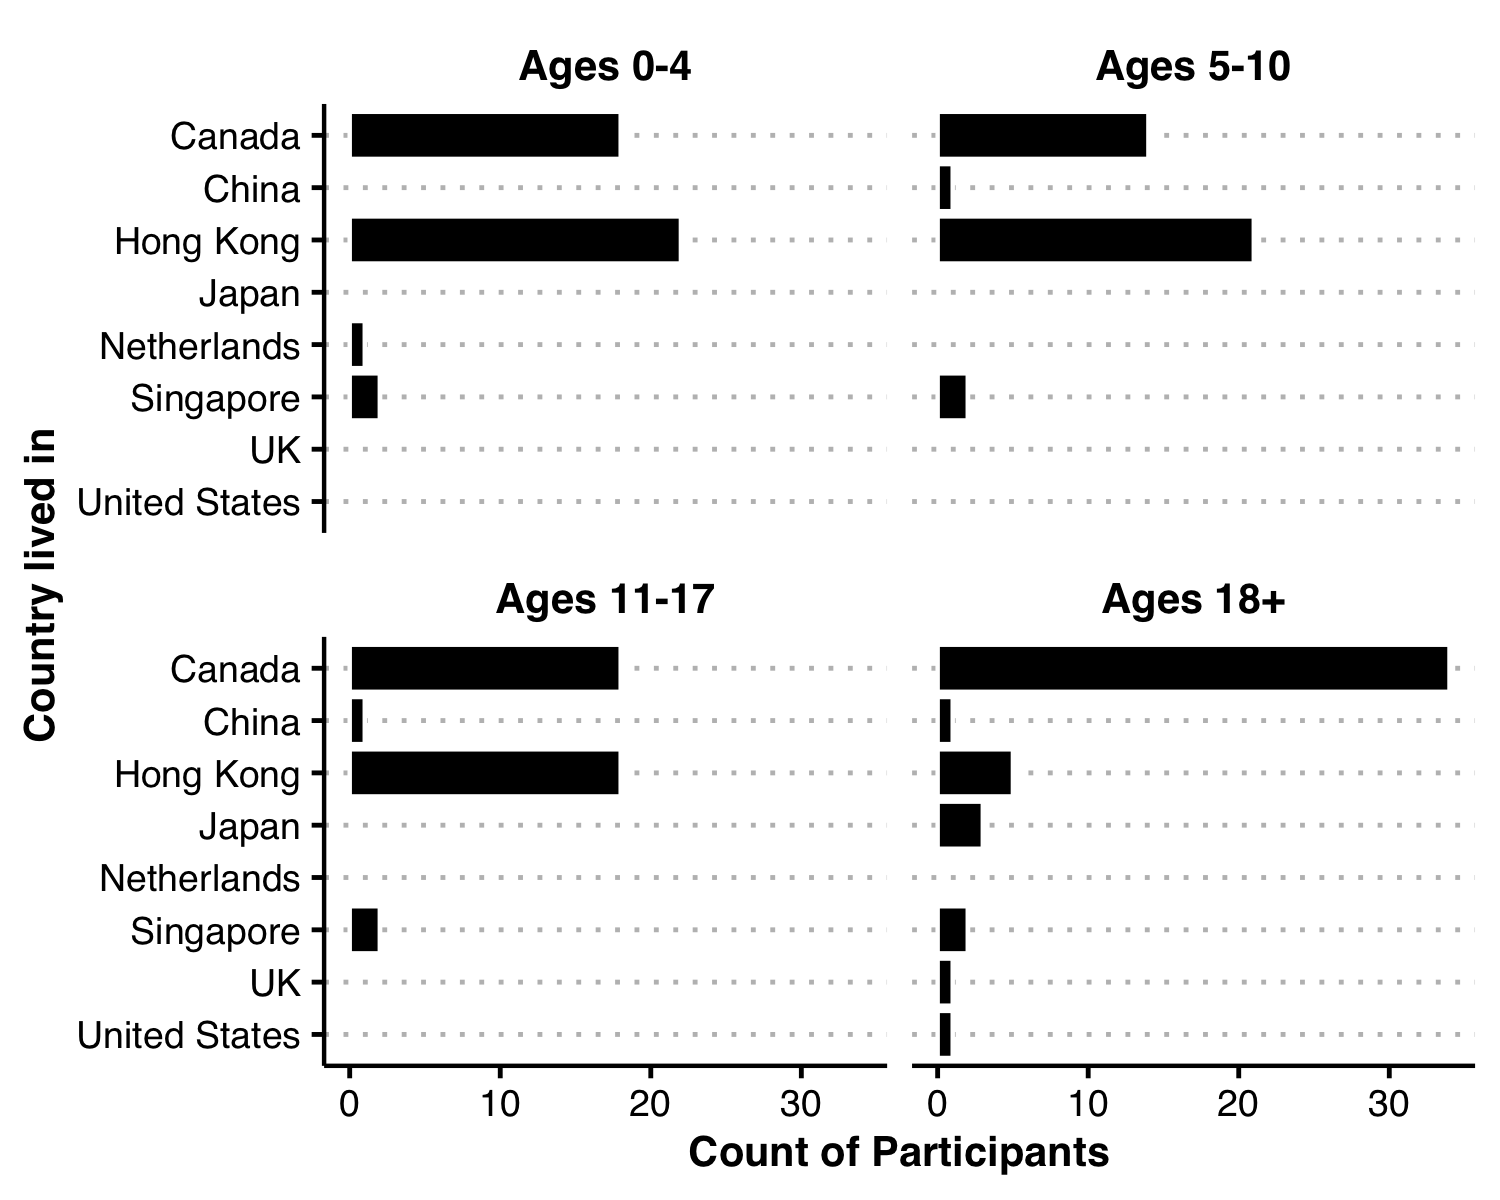
\includegraphics[width=4.9in]{figures/ch2_placeslived_5in.png} 
  \caption{This four panel bar chart summarizes where the SpiCE participants lived during different portions of their lives.}
  \label{ch2:fig:placeslived}
  \end{center}
\end{figure}

Soliciting Cantonese dialect information directly would have been challenging, as many of the participants in the corpus would not have straightforward dialect classifications. This is especially true for individual who were born and/or raised in the Cantonese diaspora, but to Hong Kongers as well, given the extent of globalization in Hong Kong \hl{(cite)}. In light of this, it is useful to summarize where the SpiCE participants' caretakers were born and raised. Figure \ref{ch2:fig:caretakers} does exactly this. The most well-represented group is Hong Kong, as 29 of 34 participants report having at least one caretaker who was primarily raised in Hong Kong. Of these, 20 report only having caretakers raised in Hong Kong. If caretakers birth location is considered instead (as in Figure \ref{ch2:fig:caretakers}), the numbers are 27 and 18, respectively. 


\begin{figure}[!htbp]
  \begin{center}
  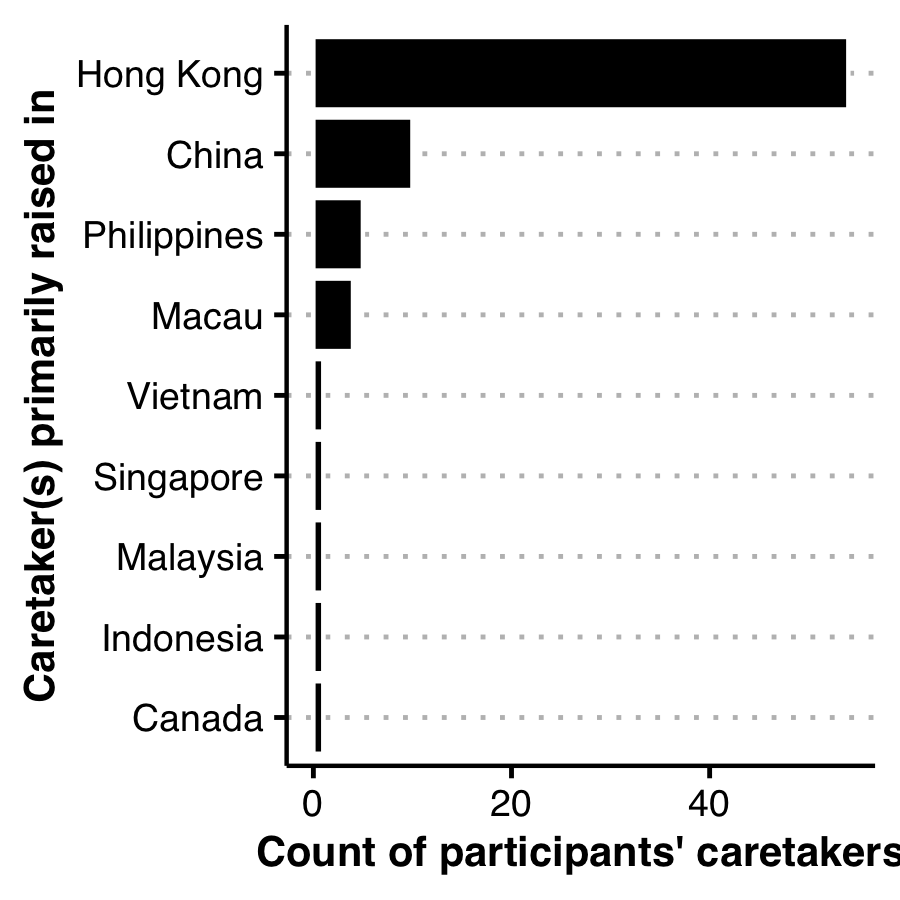
\includegraphics[width=3in]{figures/ch2_caretakers_3in.png} 
  \caption{This bar chart summarizes the number of caretakers who were born in various locations. Note that the number of caretakers reported by individual participants varies.}
  \label{ch2:fig:caretakers}
  \end{center}
\end{figure}

Additionally, calling an individual a bilingual does not preclude knowledge of additional languages. In fact, all but on of the individuals represented in the SpiCE corpus report some degree of proficiency in a language other than Cantonese or English. The most common by far is Mandarin. The age SpiCE talkers began learning other language varies widely, but is consistently later than (or simultaneous with) Cantonese and English. This information is depicted in Figures \ref{ch2:fig:multilingualism_vf} and \ref{ch2:fig:multilingualism_vm}, with a panel for each participant.

\begin{figure}[!htbp]
  \begin{center}
  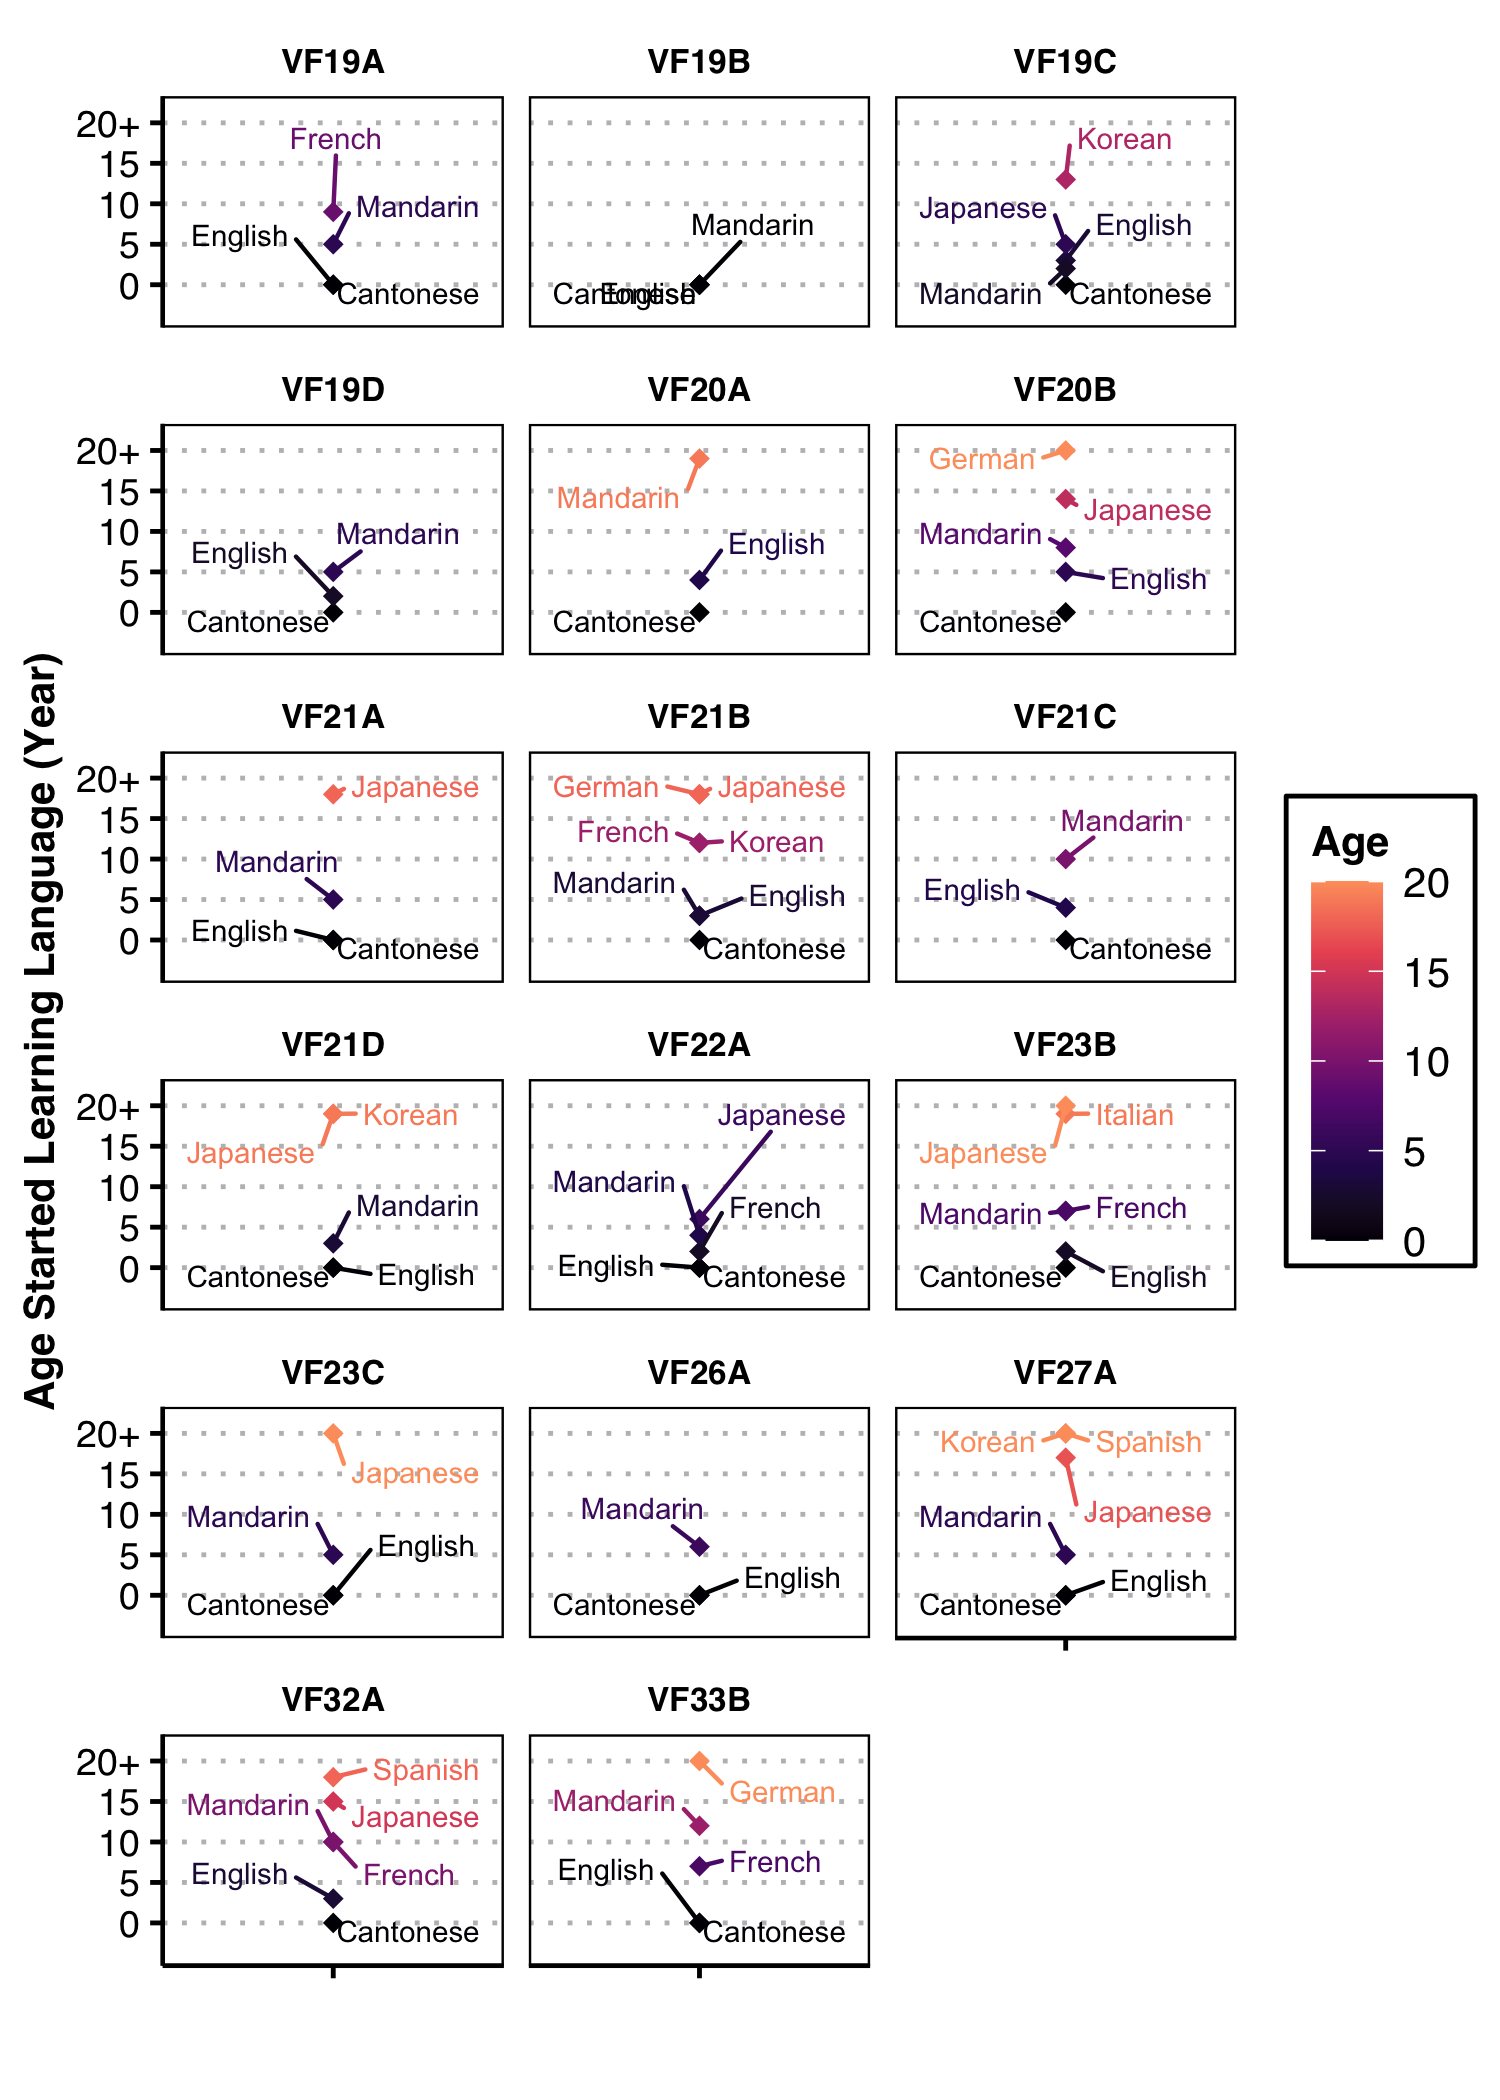
\includegraphics[width=4.5in]{figures/ch2_multilingualism_vf_5in.png} 
  \caption{Multilingualism for the female participants in the SpiCE corpus. Points represent the age that a participant began learning the language indicated in the label. Color is redundant with age, such that earlier ages are darker in color.}
  \label{ch2:fig:multilingualism_vf}
  \end{center}
\end{figure}

\begin{figure}[!htbp]
  \begin{center}
  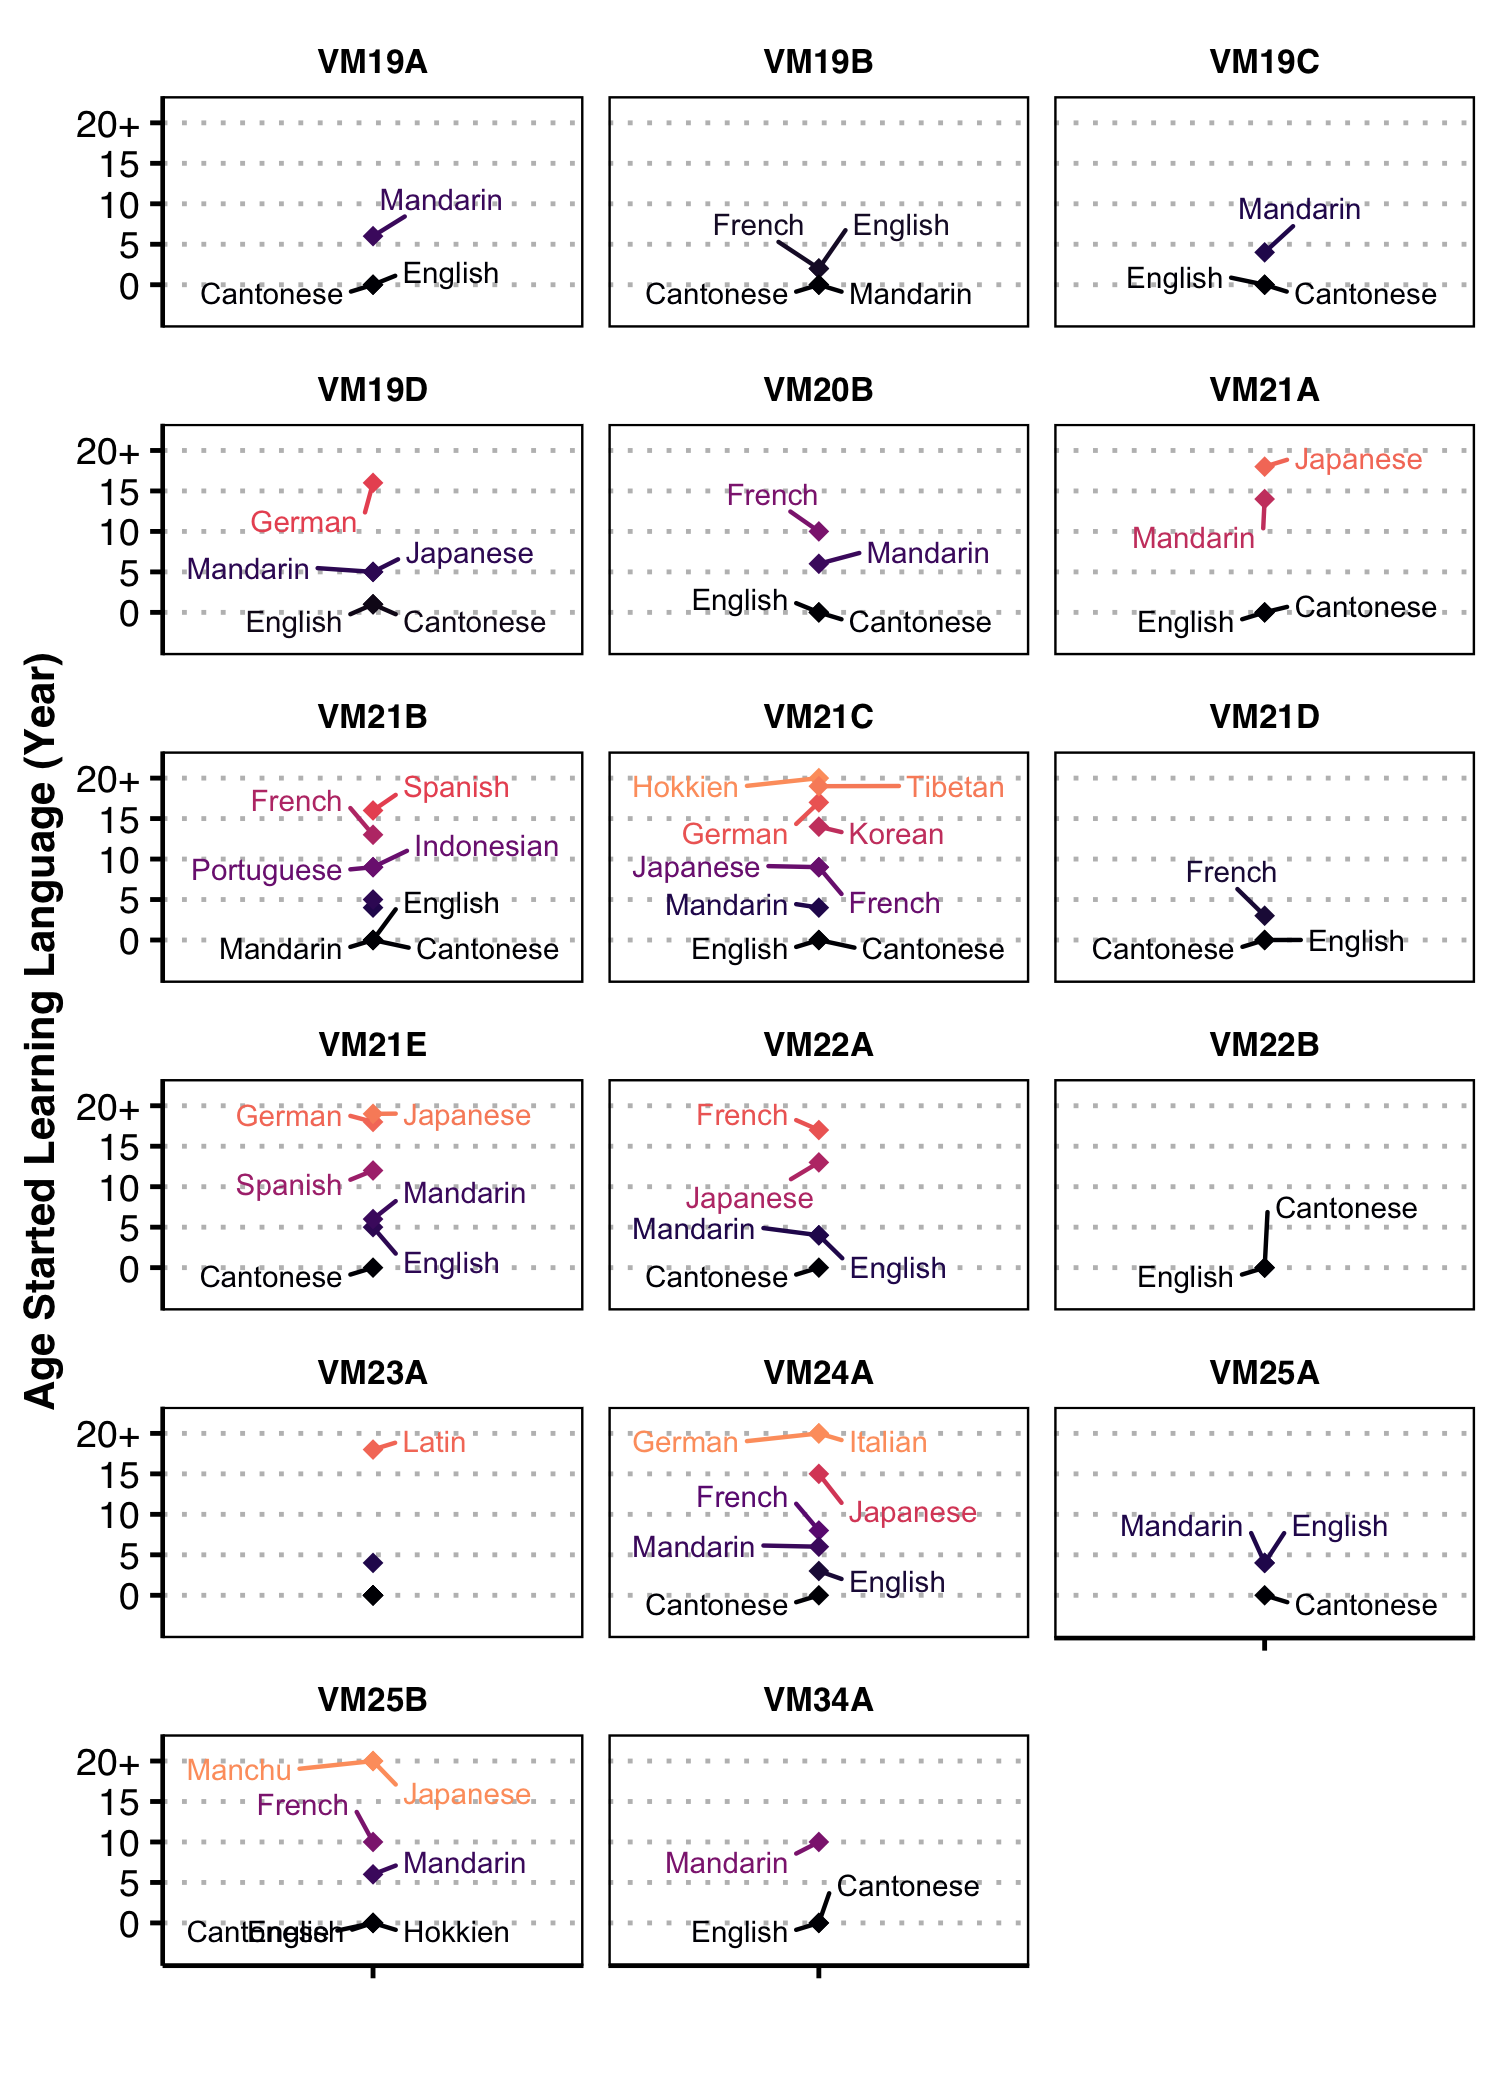
\includegraphics[width=4.5in]{figures/ch2_multilingualism_vm_5in.png} 
  \caption{Multilingualism for the male participants in the SpiCE corpus. Points represent the age that a participant began learning the language indicated in the label. Color is redundant with age, such that earlier ages are darker in color.}
  \label{ch2:fig:multilingualism_vm}
  \end{center}
\end{figure}

\subsection{Recording Setup}\label{ch2:subsec:setup}
Recording took place in a quiet room in the linguistics laboratory building at the University of British Columbia in Vancouver, Canada. Two Cantonese-English undergraduate bilingual research assistants and the participant were seated around a table. The interviewer was a female Cantonese-English bilingual from Metro Vancouver. The recording process was monitored by a male Cantonese-English bilingual from Hong Kong, who moved to Vancouver to attend university. The interviewer and participant were outfitted with AKG C520 head-mounted microphones positioned approximately 3 cm from the corner of the mouth. The microphones were connected to separate channels on a Sound Devices USBPre2 Portable Audio Interface. Stereo recordings were made with Audacity 2.2.2 \citep{audacity_2018_audio} on a PC laptop, and saved with a 44.1 kHz sampling rate, and 16-bit resolution.\footnote{Many files were originally recorded with 24-bit or 32-bit depth, but were converted to 16-bit depth prior to the publication of the SpiCE corpus, for the purporse of consistency and maintaining a reasonable file size while still providing high-quality audio.}

\subsection{Recording Procedure}\label{ch2:subsec:procedure}
Upon arrival, participants were provided with an overview of the recording session procedures, and informed of the corpus publication process. This included informing participants of the window of time in which they would be able to withdraw their data. Subsequently, participants were asked to provide written consent. Upon consent, participants completed a session in English, and a session in Cantonese. The order of languages was counterbalanced across participants (see Table~\ref{ch2:tab:participants}). Each session consisted of three tasks\textemdash sentence reading, storyboard narration, and a conversational interview\textemdash described in the following sections. Each of these three tasks were recorded in the same audio file, though there are separate recordings for each of the sessions. That is, each participant has a Cantonese session and an English session. Together, these three tasks took approximately 30 minutes in each language. Along with the consent process, recording setup, and a break between interviews, participants spent up to 90 minutes in the lab. 

\subsubsection{Sentence Reading}\label{ch2:subsec:sentences}
Participants first read the sentences listed in Table~\ref{ch2:tab:can_sent} and Table~\ref{ch2:tab:eng_sent} aloud, pausing between sentences. Participants completed a single repetition and were not instructed to speak in a particular style. As participants had varying levels of Cantonese reading ability, they were simultaneously presented with both Cantonese characters and the Jyutping romanization.\footnote{Jyutping is one of the primary Cantonese romanization systems \citep{matthews_2013_cantonese}, and is widely used in Cantonese corpus research \citep{nagy_2011_hlvc,tse_2019_heritage}} If necessary, participants could make use of the phrase's English translation. The Cantonese sentences are well-known declarative phrases, typically associated with Chinese New Year. While a more explicitly balanced set of sentences could have been used, participants' familiarity was deemed more important, as many Cantonese-English bilinguals in Canada are not literate in Cantonese. The English sentences included the Harvard Sentences list number 60 \citep{ieee_1969_sentences}, as well as series of holiday-themed declarative sentences to better match the content of the Cantonese sentences. This task was relatively formal, and typically lasted less than one minute. 

Sentence reading was included in the session to insure that different participants produced a set of identical items, considering the core of the session was unscripted conversational interview (described in Section~\ref{ch2:subsec:interview}). While these sentences do not exhaustively reflect the sound systems of Cantonese and English, they provide samples of identical items for all individuals, which is advantageous for future analyses or projects that require matched utterances.

In practice, the utility of these sentences may be somewhat limited, as sentences with speech errors were not neccessarily repeated, and some Cantonese sentences were skipped altogether. In any case, the sentence reading task also served the purpose of getting participants into the appropriate language mode prior to the upcoming interview. As such, they can be considered a warmup task. 

\begin{table}[!htbp]
\begin{center}
  \footnotesize
\begin{tabular}{c c}
\toprule
\textbf{No.}  & \textbf{English} \\
 \midrule
1 & Stop whistling and watch the boys march \\ 
2 & Jerk the cord, and out tumbles the gold \\ 
3 & Slide the tray across the glass top \\ 
4 & The cloud moved in a stately way and was gone \\ 
5 & Light maple makes for a swell room \\ 
6 & Set the piece here and say nothing \\ 
7 & Dull stories make her laugh \\ 
8 & A stiff cord will do to fasten your shoe \\ 
9 & Get the trust fund to the bank early \\ 
10 & Choose between the high road and the low \\ 
11 & Wish on every candle for your birthday \\ 
12 & Deck the halls with boughs of holly \\ 
13 & Ring in the new year with a kiss \\ 
14 & Have a spooky Halloween \\ 
15 & Enjoy the vacation with your loved ones \\ 
16 & Be filled with joy and peace during this time \\ 
17 & Relax on your holiday break \\ 
\bottomrule

\end{tabular}
\caption{Sentences 1\textendash10 comprise the Harvard Sentences List 60. Sentences 11\textendash17 are holiday-themed original imperatives, designed to thematically match the Cantonese sentences.}
\label{ch2:tab:eng_sent}
\end{center}
\end{table}

\begin{table}[!htbp]
\begin{center}
  \footnotesize
\begin{tabular}{cccc} %\begin{CJK}{UTF8}{bsmi}
\toprule
\textbf{No.} & \textbf{Cantonese} & \textbf{Jyutping} & \textbf{English translation} \\ 
\midrule
1 & 新年快樂 & \textit{san1 lin4 faai3 lok6} & Happy New Year \\ 
2 & 恭喜發財 & \textit{gung1 hei2 faat3 choi4} & Congratulations on happiness and prosperity \\ 
3 & 身體健康 & \textit{san1 tai2 gin6 hong1} & May your health be well \\ 
4 & 快高長大 & \textit{faai3 gou1 zoeng2 dai6} & Grow quickly \\ 
5 & 龍馬精神 & \textit{lung4 ma5 zing1 san4} & Have the spirit of the horse and dragon \\ 
6 & 學業進步 &\textit{ hok6 yip6 zeon3 bou6} & Progress in your education \\ 
7 & 年年有餘 & \textit{lin4 lin4 yau5 yue4} & Excess in each year \\ 
8 & 出入平安 & \textit{cut1 yap6 ping4 on1} & Leave and enter in safety \\ 
9 & 心想事成 & \textit{sam1 soeng2 si6 sing4} & Accomplish that which is in your heart \\ 
10 & 生意興隆 & \textit{saang1 yi3 hing1 lung4} & Have a prosperous business \\ 
11 & 萬事如意 & \textit{maan6 si6 yu4 yi3} & A thousand things according to your will \\ 
12 & 天天向上 & \textit{tin1 tin1 hoeng3 soeng6} & Upwards and onwards every day \\ 
13 & 笑口常開 & \textit{siu3 hau2 soeng4 hoi1} & Laugh with an open mouth frequently \\ 
14 & 大吉大利 & \textit{daai6 gat1 daai6 lei6} & Much luck and much prosperity \\ 
15 & 五福臨門 & \textit{mm5 fuk1 lam4 mun4} & Five blessings for your household \\ 
16 & 招財進寶 & \textit{ziu1 coi4 zeon3 bou2} & Seek wealth welcome in the precious \\ 
17 & 盤滿砵滿 & \textit{pun4 mun5 but3 mun5} & Basins full of wealth \\ 
\bottomrule
\end{tabular}
\caption{All Cantonese sentences are widely-known imperatives associated with Chinese New Year.}
\label{ch2:tab:can_sent}
\end{center}
\end{table}

\subsubsection{Storyboard Narration}\label{ch2:subsec:storyboard}
For the second task, participants narrated a short story from a cartoon storyboard originally developed for linguistic field work \citep{littell_2010_thank}. The storyboard followed a simple plot about receiving gifts and writing thank you notes to family members and friends\textemdash a topic that Cantonese-English bilinguals in the corpus were expected to be familiar with in both languages. This task was less formal than the sentence reading task, and ensured that different participants produced some of the same words in a more spontaneous context. Participants varied in how they approached this task, with some treating it like a serious of picture description tasks, and others taking a more narrative approach. Despite this difference, this task may be useful for future analyses or projects that require matched utterances, as participants narrated the same cartoon in each language. This ensured that some of the same content was conveyed in each language (e.g., productions of \textit{mother} in both languages). The storyboard narration lasted 4\textendash5 minutes in each session, and allowed participants time to continue getting used to the recording setup. As with the sentences, the storyboard narration also facilited participants getting into the language mode of the session prior the the conversational interview. This is important, because language mode is known to affect the degree of crosslinguistic influence in speech production \citep{simonet_2019_convergence}.

\subsubsection{Conversational Interviews}\label{ch2:subsec:interview}
The conversational interviews formed the bulk of the recording time for each participant, lasting around 25 minutes. Participants were informed of the general interview structure ahead of time. The casual interview format was inspired by the Buckeye corpus of conversational speech \citep{pitt_2005_buckeye}, and included everyday topics such as family, school, culture, hobbies, and food. These topics were selected to be relevant, interesting, and encourage storytelling, but to not delve into the personal details typically elicited in a sociolinguistic interview \citep{nagy_2011_hlvc}. A major goal was for participants\textemdash who knew they were being recorded for linguistic inquiry\textemdash to feel at ease and freely discuss the questions. Questions were loosely laid out under general topic headings, with optional follow-up questions. While the English and Cantonese interviews had the same structure and general topic areas, the particular questions differed. Furthermore, each interview took its own shape, and was guided by what the participant wanted to talk about, anywhere from three to six topic areas covered---the planned sequence of questions is included in the Appendix. As a result, the speech samples from each language are comparable, but the specific questions differ between interviews and across participants. 

Participants were encouraged to code-switch between languages by the interviewer, who included code-switches in some of her questions, and asked about topics that encouraged switches (e.g., Chinese foods in English; university course work in Cantonese). While code-switching was encouraged, it was not a primary focus for the session. As will become apparent later in this chapter, there was substantially more code-switching in the Cantonese part of the session.

\begin{figure*}[ht]
\begin{center}
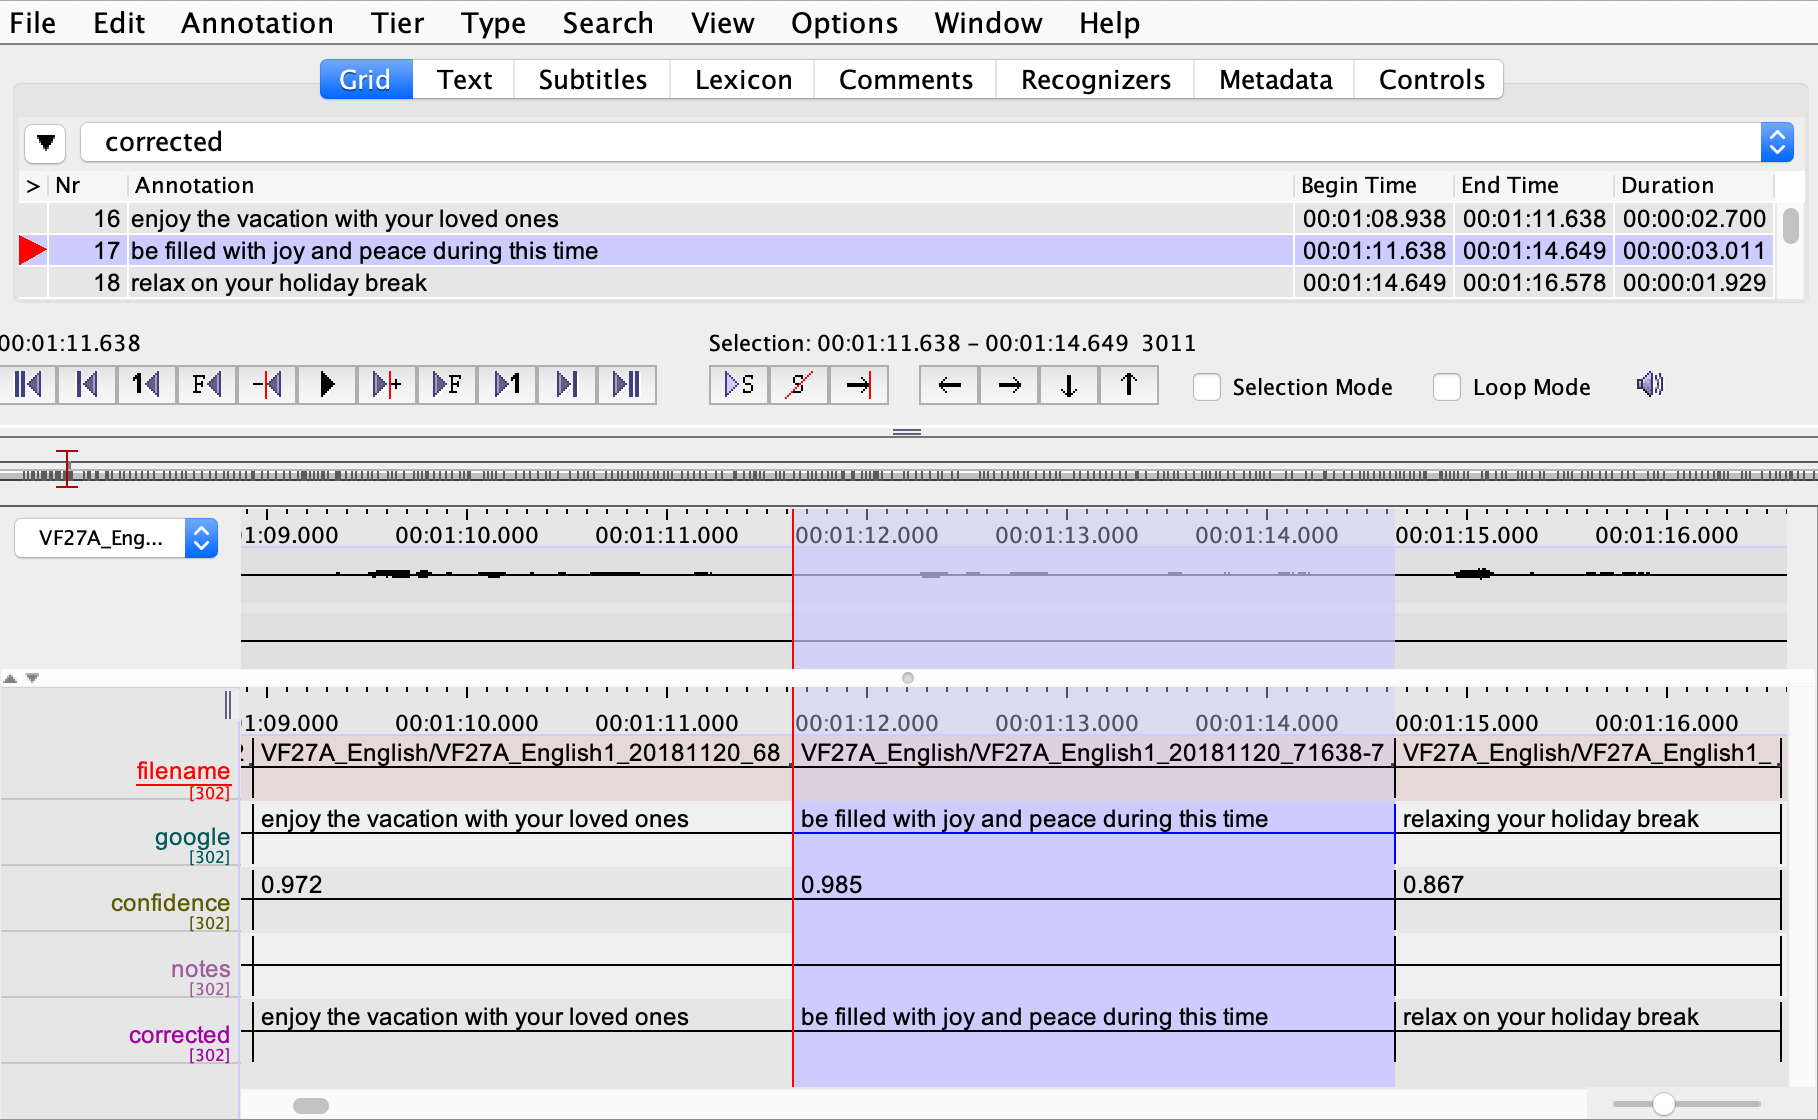
\includegraphics[width=4.9in]{figures/ch2_elan.png} 
\caption{This screenshot from ELAN shows a sample of hand-corrected English from the sentence reading task for participant VF27A. The audio waveform is displayed in two channels, with one for the participant (top) and the other for the interviewer (bottom). The annotation tiers include (1) the short audio chunk's filename, (2) the raw speech-to-text transcript, (3) the speech-to-text confidence rating, (4) space for transcriber notes, if any, and (5) the corrected transcript. Note that ``relaxing'' was corrected to ``relax on'' in the rightmost section displayed.}
\label{ch2:fig:elan}
\end{center}
\end{figure*}

\section{Annotation}\label{ch2:sec:annotation}
All recordings were processed according to the pipeline outlined in this section. As much as possible, automatic tools were leveraged to expedite hand correction. 

\subsection{Cloud Speech-to-Text}\label{ch2:subsec:stt}
Google Cloud Speech-to-Text was used to produce an initial transcript of the interviews \citep{google_2019_stt}. This was done using the Short Audio option, with the language variety set to Canadian English (en-CA) or Hong Kong Cantonese (yue-Hant-HK). In order to use this speech recognition product, the participant's speech was extracted from the participant's channel and segmented into short chunks, typically under 15 seconds in duration.\footnote{The interviewer's speech is included in the SpiCE corpus recordings for the purpose of context, but is not transcribed.} No attention was paid to constituents at this point; rather, breaks were placed at breaths and other pauses. Short chunks were necessary in order to use the speech recognition product with locally stored files, which was important for data privacy reasons. The short chunks would also prove useful for transcribers in the subsequent hand correction phase. With the audio files prepared in this way, speech recognition was completed using the Python client library for Google Cloud Speech-to-Text. The output included both a transcript and a confidence rating for each audio chunk. While the transcripts generated in this fashion were far from perfect, they served the function of expediting the hand-correction process.

\subsection{Orthographic Transcription Hand-Correction}\label{ch2:subsec:orthographic}
The automatically generated transcripts were converted into multi-tiered ELAN transcription files \citep{sloetjes_2008_elan}, with tiers for the automatically generated transcript, phrase transcription confidence, notes, and corrected transcript. During hand-correction, research assistants adjusted the transcript in the corrected tier, and took note of anything pertinent to the given audio chunk. Figure~\ref{ch2:fig:elan} depicts an example of corrected English transcriptions in ELAN \citep{sloetjes_2008_elan}. Direct identifiers (e.g., names) were marked during this phase, and silenced from the recordings prior to release. Transcriber guidelines were adapted from the multilingual Heritage Language Variation and Change corpus, which includes Cantonese \citep{nagy_2011_hlvc}. Guidelines for Cantonese were developed in collaboration with the bilingual research assistant team.

In both languages, the following conventions were used:
\begin{itemize}
 \item The placeholder ``xxx'' denotes unintelligible speech.
 \item Fragments are transcribed using ``\&'' followed by the fragment produced (e.g., ``\&s'').
 \item The ``?'' symbol marks questions but is not used consistently; other punctuation is not used.
\item Words produced in a language other then English or Cantonese are transcribed in the language with, for example, ``@m'' appended to the end of each form for Mandarin (simplified characters), ``@j'' for Japanese, and similar. 

\end{itemize}

Cantonese-specific conventions include:
\begin{itemize}
 \item Where possible, transcription is in characters.
 \item Words without a standard character are transcribed in the Jyutping romanization system (e.g., \textit{jyut6ping3}).
 \item Fully-lexicalized syllable fusion is transcribed with the typical smaller number of characters (e.g., 咩 \textit{me1} is a fully fused version of 乜嘢 \textit{mat1 ye5}, and intermediate version 咩嘢 \textit{me1 ye5}\textemdash all translate to ``what'').\footnote{Syllable fusion is a phenomenon in which adjacent syllables in Cantonese are blended together. It ranges from assimilation at the syllable boundary to segment deletion and re-syllabification \citep{wong_2006_fusion}. Syllable fusion is common in Cantonese, though its frequency of occurrence and degree varies.}
 \item Non-lexicalized (or ambiguous) cases of syllable fusion are transcribed with the full number of characters fused (e.g., 朝頭早, ``morning,'' is fully pronounced as \textit{ziu1 tau4 zou2}, but can be fused to 【朝頭】早 \textit{ziau14 zou2}. Brackets indicate the fused syllables).
 \item Filled pauses are transcribed with the character 㖡 (\textit{e6}), or using Jyutping if different (e.g., \textit{m6}). 
 \item Transcribers followed a shared set of guidelines for transcribing sentence final particles.
\end{itemize}

English-specific conventions include:
\begin{itemize}
 \item Standard spelling is used.
 \item Proper nouns are capitalized (e.g., ``British Columbia''). 
 \item Filled pauses are transcribed with ``um'', ``er'', ``uh'', and other similar, non-elongated forms.
 \item Numbers are written out in word form (e.g., ``one hundred'').
\end{itemize}

\subsection{Forced Alignment}\label{ch2:subsec:alignment}
Force-aligned transcripts were produced with the Montreal Forced Aligner \citep{mcauliffe_2017_mfa}, using the hand-corrected orthographic transcripts. 

In Cantonese, forced alignment was completed with the Train-and-Align option, as there was no pretrained model available for Cantonese. As Cantonese orthpgraphy does not separate words with spaces, words segmentation was done using the \textit{jieba} Python library \citep{sun_2020_jieba}, along with a Cantonese dictionary.\footnote{The Cantonese Word Segmentation GitHub page: \url{https://github.com/wchan757/Cantonese_Word_Segmentation}.} While using an automated tool such as this is likely an imperfect solution, it has the benefit of reproducibility and consistency. This is important, as it can be difficult to define wordhood in Cantonese \citep[e.g., see][]{wong_2006_fusion}.

The Cantonese pronunciation dictionary was generated using the \textit{PyCantonese} Python library \citep{lee_2018_pycantonese}. Pronunciations were identified by getting the Jyutping romanization from each character (or using the Jyutping transcribed), separating it into segments, and appending the tone number to the syllable nucleus (i.e., vowel or syllabic nasal). Research assistants supplemented the dictionary with alternative pronunciations for words that participated in syllable fusion. This approach bears some similarity to that of \citet{tse_2019_heritage}, but differs in that it also includes tonal information---which has been shown to improve forced alignment as long as there are not too many tone-nucleus combinations \citep{cavar_2016_endangered, yuan_2014_automatic}. %maybe add a DiCanio reference, see Matt Faytak's email

Forced alignment in English took advantage of the Montreal Forced Aligner's pretrained English model and pronunciation dictionary, which broadly reflects North American English varieties. The dictionary was supplemented with manual additions, in order to minimize the number of out-of-vocabulary items.

The word and phone output of the forced alignment process was included in a TextGrid for each audio recording, along with annotation tiers for task (sentences, storyboard, or interview), utterance (the short chunks). In both sessions, any material not in the main language of the session was not force aligned, and appears as ``<unk>'' for unknown in the word tier and ``spn'' in the phone tier. The force-aligned transcripts were not manually corrected or checked. This means that any short chunk with code-switching or unintelligible speech will likely have poorer alignment. As a result, it is advisable to use stringent exclusionary criteria or perform checks prior to analyzing data from the corpus. 

\section{Descriptive Statistics}\label{ch2:sec:statistics}
The descriptive statistics in this section are intended to give a general sense of the quantity and quality of the data in the corpus. They are based on the transcript data as described in the previous section, specifically the hand-corrected utterance tier, and the force-aligned phone tier. Additionally, this section only reports on participant speech, though the interviewer's speech is included in its own channel in the stero audio files.

\subsection{Cantonese Interviews}\label{ch2:subsec:cantonese_descriptive}

The Cantonese recordings include 8.3 hours of speech: 13.6 minutes of sentences, 44.0 minutes of storyboard narration, and 7.4 hours of conversational interview. These estimates are calculated from the summed duration of all non-silent intervals in the phone tier of the transcripts, and as such, do not include interviewer questions or any pauses in the participant's speech. 

\begin{figure}[!htbp]
  \begin{center}
  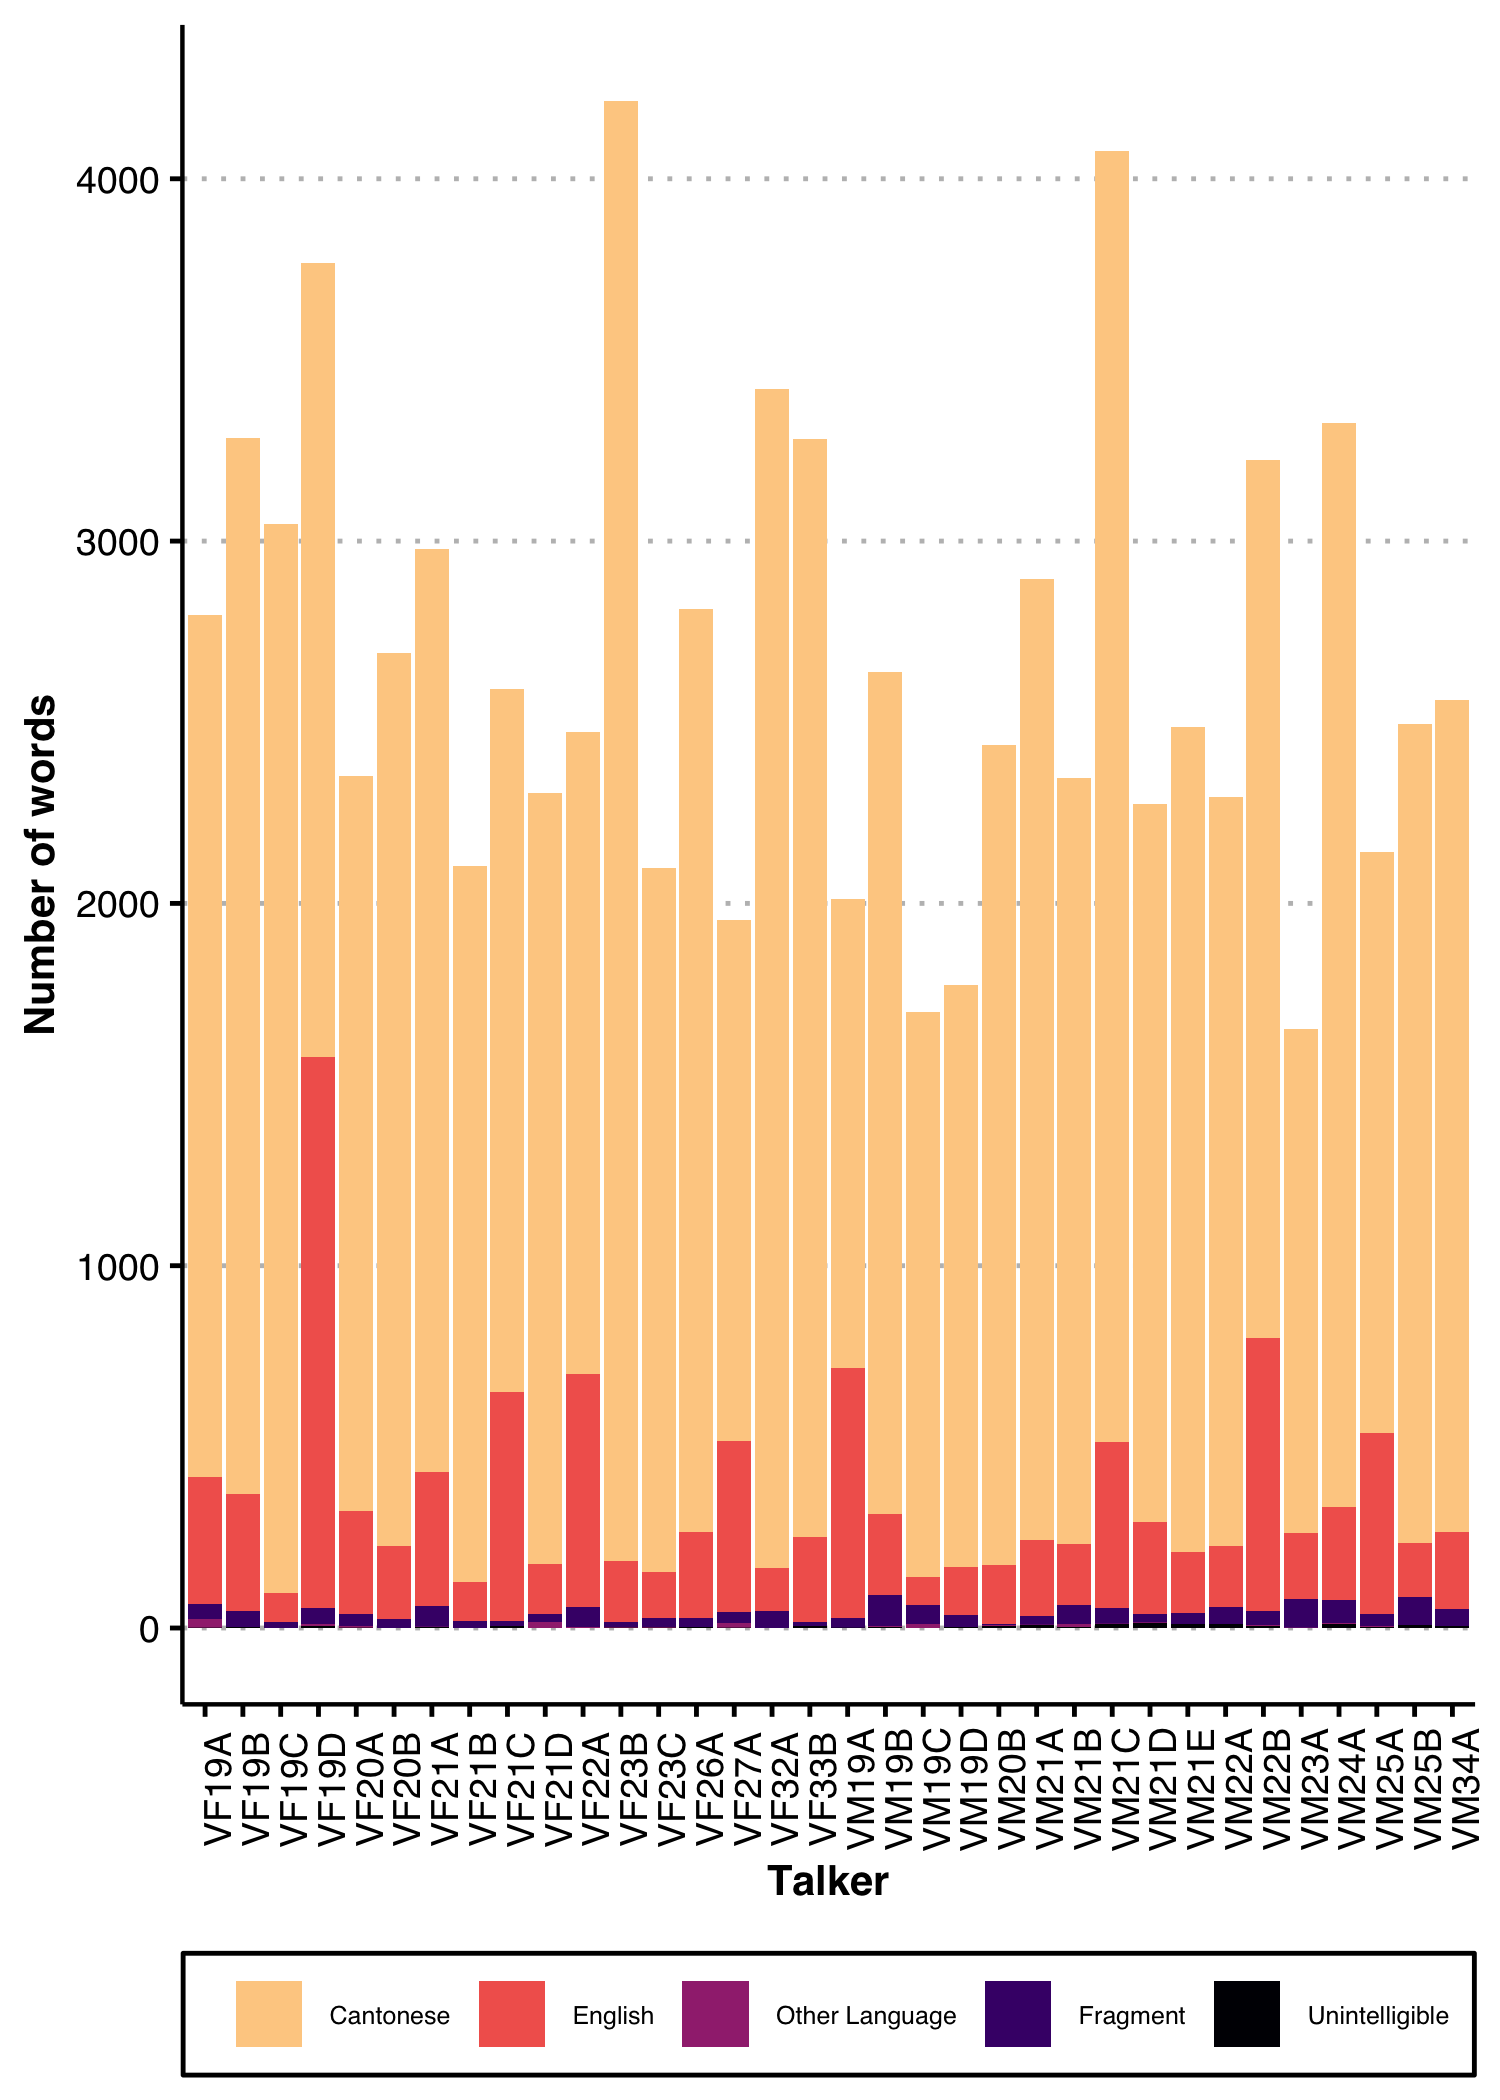
\includegraphics[width=4.9in]{figures/ch2_cantonesetypecounts_5in.png} 
  \caption{The total word count for each participant's Cantonese interview task is represented by bar height. Color indicates the kind of item counted. }
  \label{ch2:fig:cantonesetypecounts}
  \end{center}
\end{figure}

In the Cantonese interview sessions, there were a total of 8,112 word types, and 90,512 word tokens. The number of words varies substantially by participant, with a mean of 2,662 word tokens per interview (SD$=$637, minimum$=$1,654, maximum$=$4,212), and 749 word types (SD$=$157, minimum$=$483, maximum$=$1081). The numbers reported here include all types of ``words''---Cantonese words, English words, words in other languages, phonological fragments, and unintelligible stretches of speech. Figure \ref{ch2:fig:cantonesetypecounts} shows split of these categories on a by-participant basis within the Cantonese interview sessions. Figure \ref{ch2:fig:cantonesetypecounts} indicates that all participants switch into English during the Cantonese interview sessions. The amount of switching varies across participants, with VF19D producing an especially large number of English words. While the other three categories also vary, they are comparatively small in number. 

The overall distribution of word frequency in the Cantonese interviews is depicted in Figure~\ref{ch2:fig:cantonesewordfrequency}. As expected, there are a relatively small number of words occurring frequently (e.g. pronouns, function words, etc.), while a majority are mid and low frequency. This pattern follows what is expected in a word frequency distribution, and is reassuring given the automated method of segmenting the Cantonese transcripts into words. 

\begin{figure}[h]
  \begin{center}
  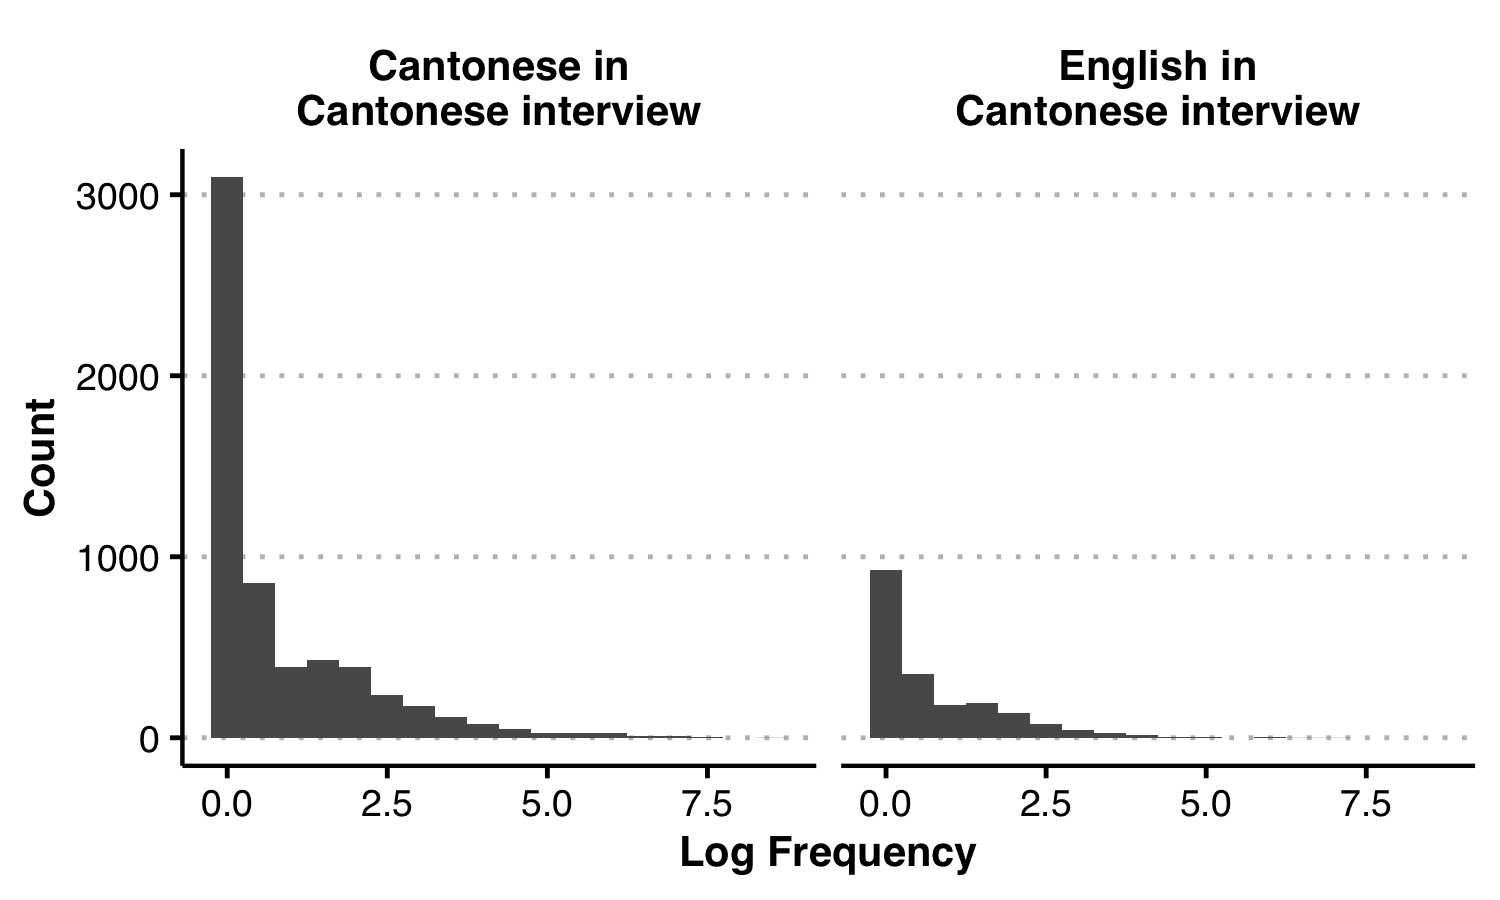
\includegraphics[width=4.9in]{figures/ch2_cantonesewordfrequency_5in.png} 
  \caption{The distribution of log word frequency for English and Cantonese words in the Cantonese interviews.}
  \label{ch2:fig:cantonesewordfrequency}
  \end{center}
  \end{figure}

\subsection{English Interviews}\label{ch2:subsec:english_descriptive}

Using the same estimation technique as used for Cantonese, the English recordings include 8.9 hours of speech: 21.9 minutes of sentences, 45.7 minutes of storyboard narration, and 7.7 hours of conversational interview speech.

The English interviews include a total of 4,972 word types and 104,618 word tokens. As in the Cantonese interviews, the number of words varies substantially by participant, with a mean word token count of 3,077 (SD$=$701, minimum$=$1,907, maximum$=$4,240), and word type count of 609 (SD$=$119, minimum$=$434, maximum$=$904). Figure \ref{ch2:fig:englishtypecounts} shows split of these categories on a by-participant basis within the English interview sessions. Unlike the Cantonese interviews, there were relatively few switches into Cantonese, with 12 of the 34 participants producing fewer than 10 Cantonese words during the English sessions.

The distribution of log word frequency for both Cantonese and English words in the English interviews is portrayed in Figure~\ref{ch2:fig:englishwordfrequency}. Word frequency follows a similar pattern to Cantonese word frequency, with most words occurring infrequently, and a smaller proportion occurring very frequently.

\begin{figure}[h]
  \begin{center}
  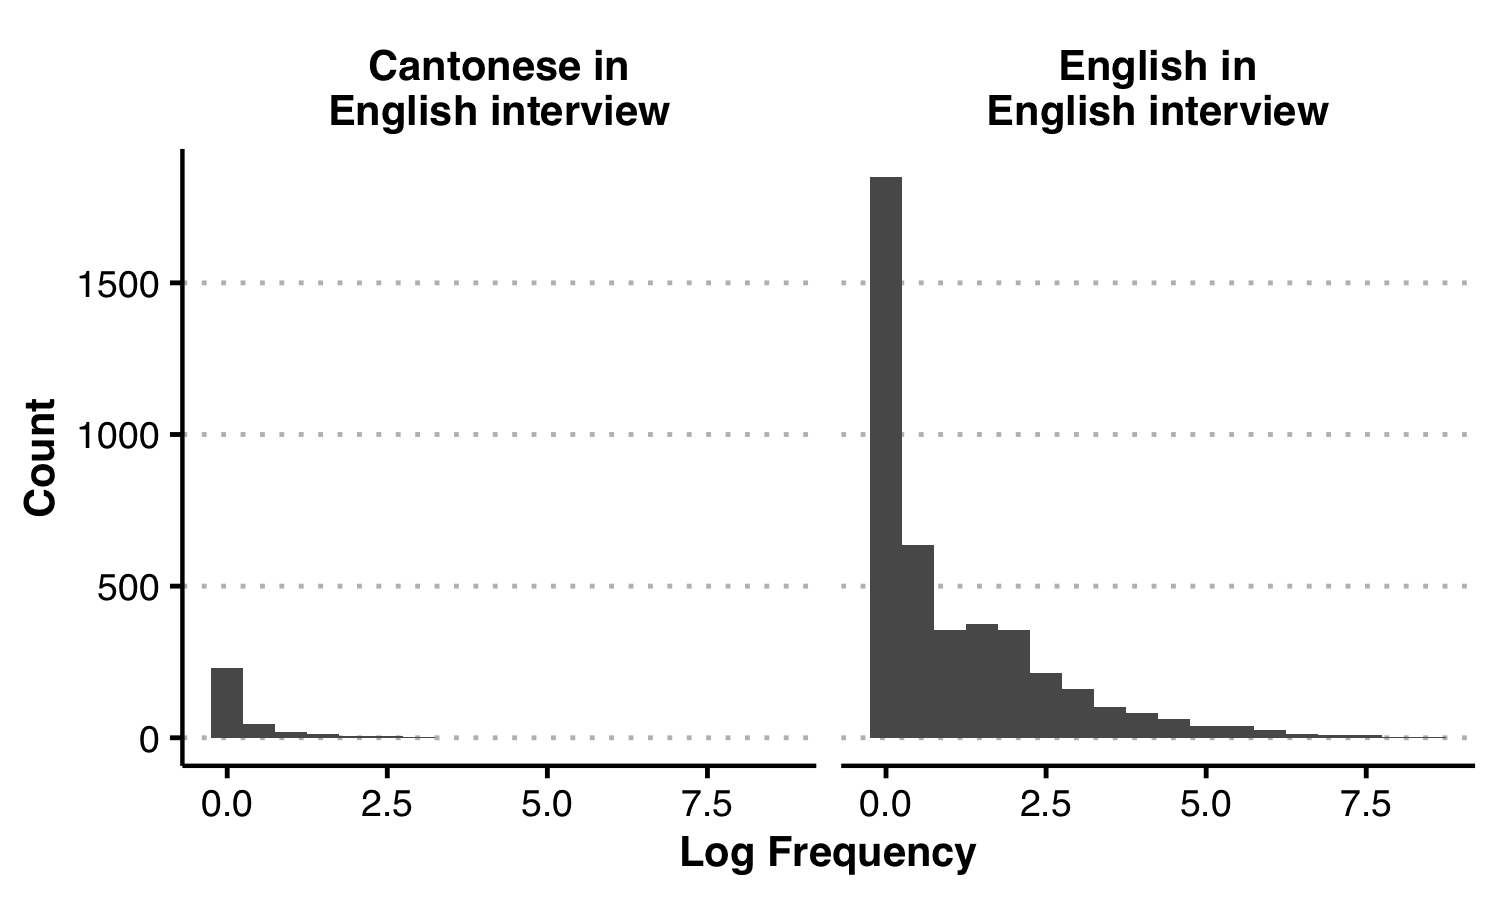
\includegraphics[width=4.9in]{figures/ch2_englishwordfrequency_5in.png} 
  \caption{The distribution of log word frequency for English and Cantonese words in the Cantonese interviews.}
  \label{ch2:fig:englishwordfrequency}
  \end{center}
\end{figure}

\begin{figure}[!htbp]
  \begin{center}
  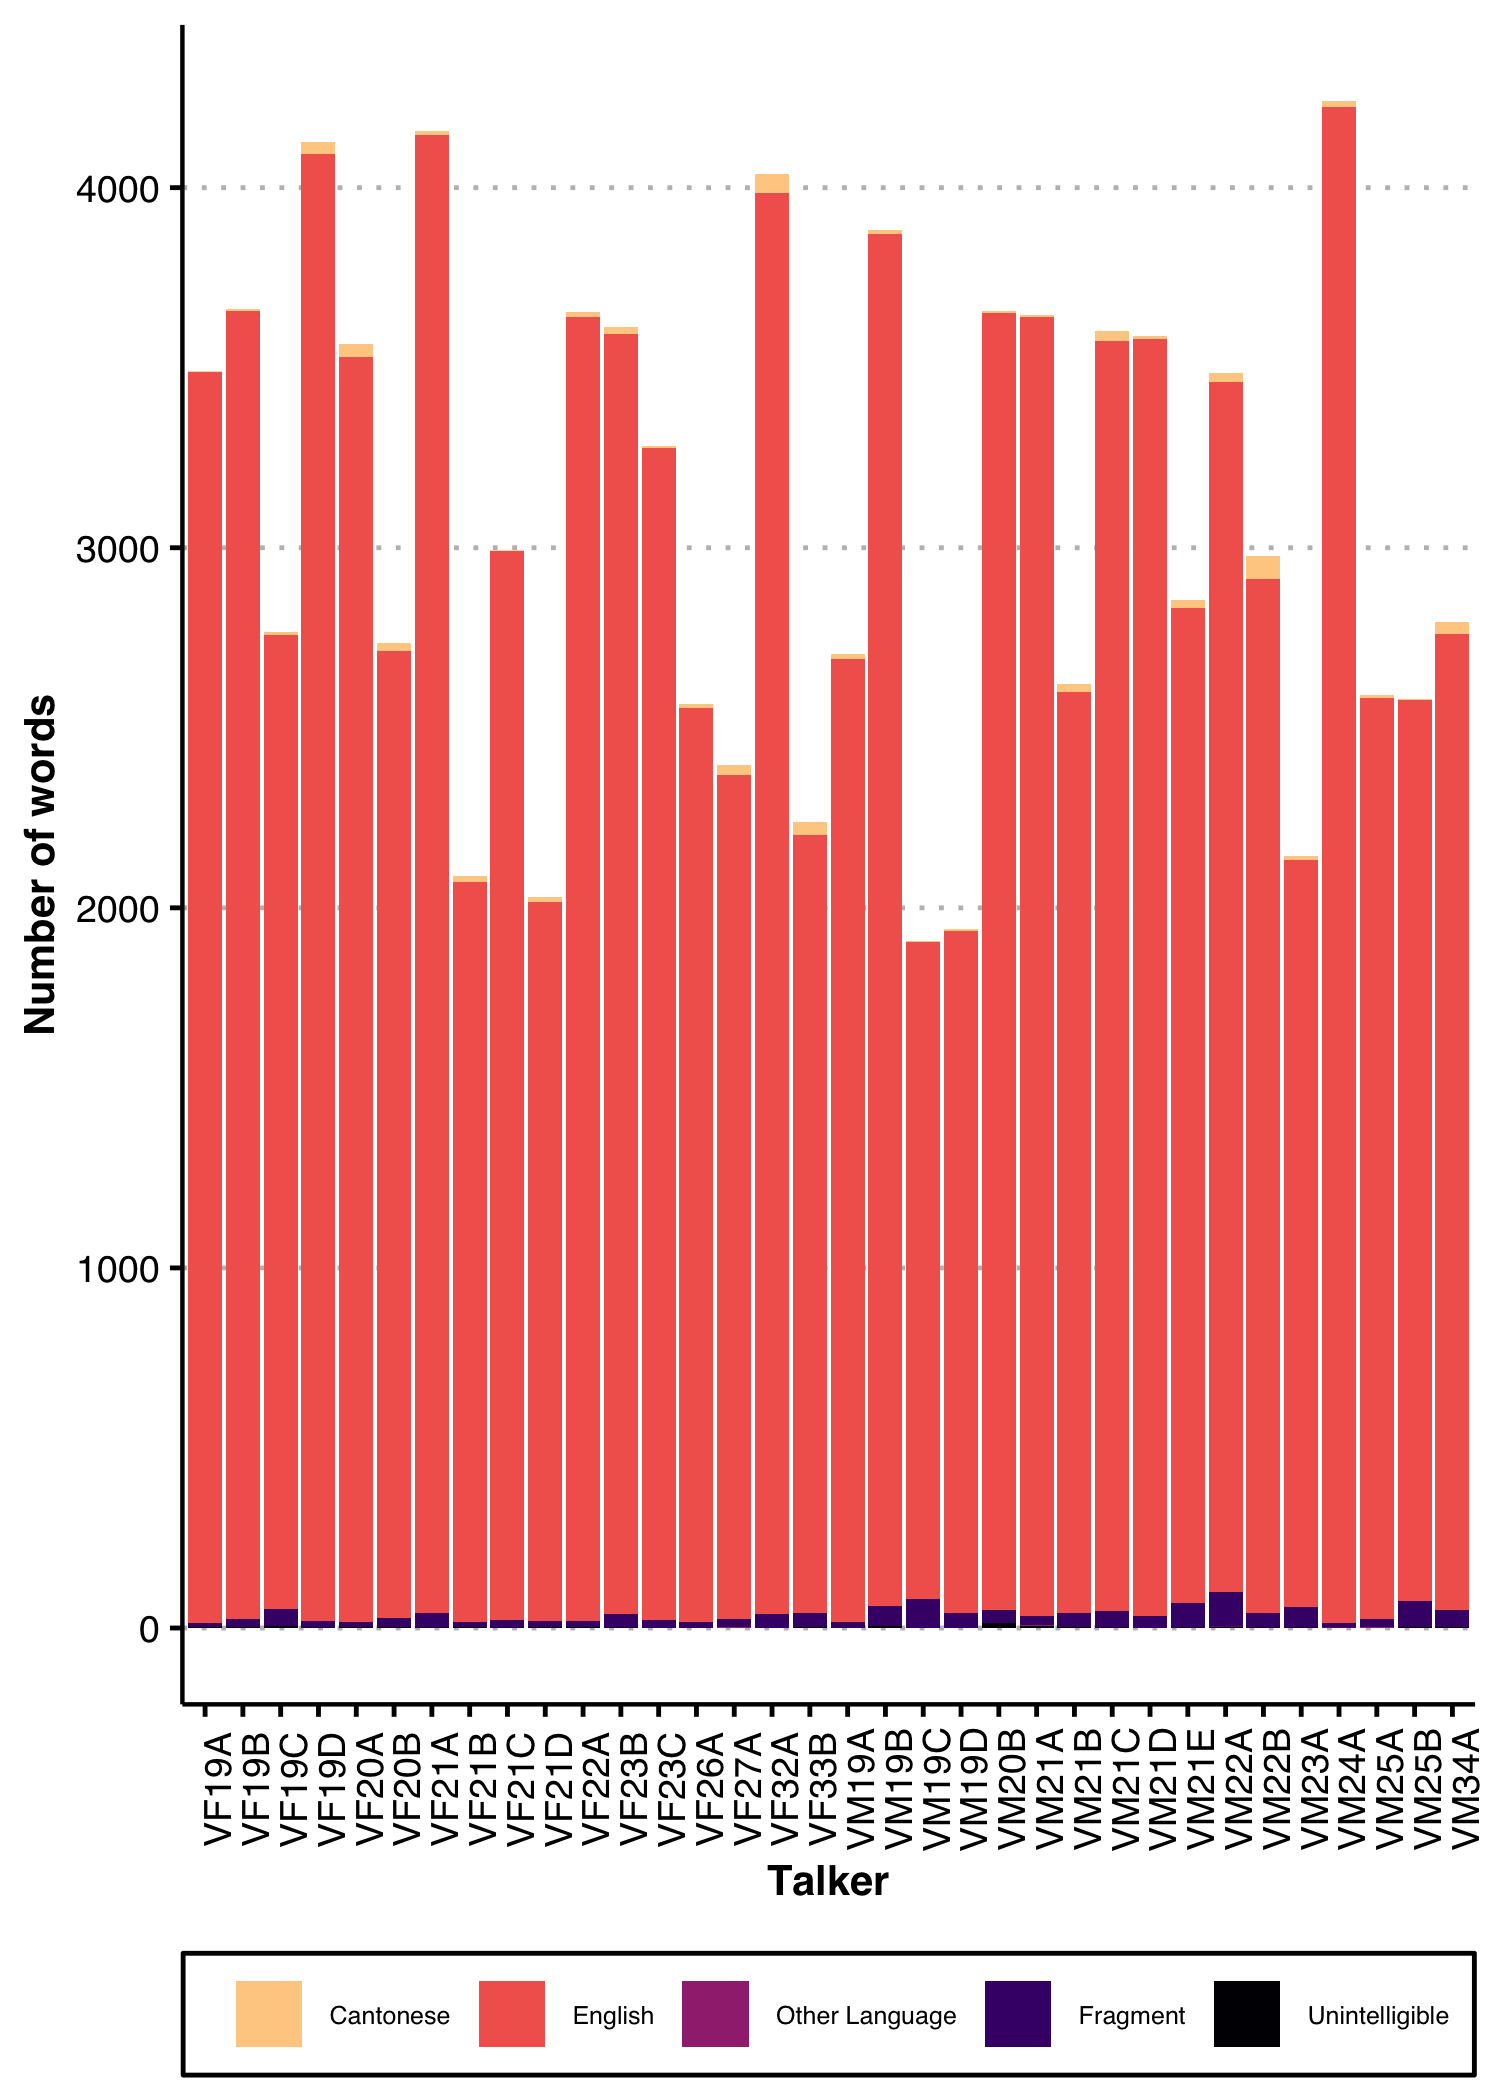
\includegraphics[width=4.9in]{figures/ch2_englishtypecounts_5in.png} 
  \caption{The total word count for each participant's English interview task is represented by bar height. Color indicates the kind of item counted. }
  \label{ch2:fig:englishtypecounts}
  \end{center}
\end{figure}

\section{SpiCE Corpus Release}\label{ch2:sec:releases}

The SpiCE corpus was publicly released in May 2021 through the Scholars Portal Dataverse platform under a Creative Commons Attribution 4.0 International License.\footnote{\url{https://creativecommons.org/licenses/by/4.0/}} In addition to the corpus itself, documentation is available online.\footnote{https://spice-corpus.readthedocs.io/}

\section{Discussion \& Conclusion}\label{ch2:subsec:discussion}

While various bilingual corpora exist, they lack in different ways. The SpiCE corpus described here enables within-speaker phonetic comparisons across languages. While this would be possible with some of the bilingual speakers in resources like the Bangor corpora \citep{deuchar_2014_corpora}, the recording quality in such resources limits the scope of phonetic research. With the release of SpiCE and its high-quality recordings, scholars have the ability to ask and answer empirically and theoretically motivated research questions within the speech and language sciences using more sophisticated phonetic measurement techniques (e.g., spectral measures, in addition to temporal measures). This offers substantial potential for increasing our understanding of bilingual spoken language from both phonetic and psycholinguistic perspectives. While the recording quality of this corpus offers these particular advantages, SpiCE is also suitable for any other standard corpus-based inquiry with conversational speech, whether linguistic or paralinguistic in nature. The opportunities made available with SpiCE are especially important given the typological difference between the languages under consideration, and the fact that Cantonese is an understudied language. 

\endinput % -------------------------------------------------------- %

%%!TEX root = dissertation.tex

\chapter{The structure of acoustic voice variation in bilingual speech}
\label{ch3:Voice}


% add a structure in variability section so i can cite the face stuff in the intro

\section{Introduction}\label{ch3:sec:introduction}
Voices provide a lot of information about the person talking, ranging from their current physical and emotional state to talker indexical features that help listeners identify who they are. In this context, voices can be described as auditory faces, in that they are uniquely individual, yet share basic characteristics with the broader population \citep{belin_2004_voice}. Voices convey this rich array of information along with the message being communicated. Understanding the structure of a voice is no small feat, as is understanding how listeners use different dimensions within the voice in processing talker indexical, affective, social, and linguistic information. The difficulty here arises from the sheer variability across voices. While voices share attributes and relevant acoustic dimensions, much of the variation across voices appears idiosyncratic \citep{lee_2019_acoustic}. From the perspective of voice perception, the balance between shared and idiosyncratic characteristics makes sense. The shared dimensions allow listeners to perceive, classify, and understand new voices, while the idiosyncrasies enable identification and discrimination between voices. While this makes sense conceptually, understanding the structure of voice variation in speech production and its complement in listeners' ability to process that information remains an active area of research. While the focus of this chapter is acoustic voice variability, the emphasis on describing and processing variation echoes one of the big puzzles in phonetics: the ``lack of invariance'' problem \citep{liberman_1967_perception}. That is, given the ubiquity of variation, how do perceivers efficiently extract relevant and important information from the communicative signal? This chapter foregrounds the signal itself, asking what is available in the signal for listeners to use. 

While variation is indeed wide-ranging, it remains far from random. Some of the most prevalent accounts of how individuals understand and process variation emphasize that variation in speech production is highly structured. This chapter looks at the structure of voices, and the following chapter examines structure for sound categories---both attempt to elucidate what exists in the signal for listeners to use.  In the domain of voice quality, Jody Kreiman and colleagues have synthesized work from various areas and put forth a psychoacoustic model of voice quality \citep{kreiman_2014_theory}. This model features a minimal set of acoustic dimensions necessary to encode (and thus reproduce) voice quality. While there are numerous dimensions in the model, extensive experimental work has validated the inclusion of each dimension \citep[][and references therein]{kreiman_2021_validating}. As a result, Kreiman and colleagues argue that this set is both sufficient and necessary to capture a wide range of normal and disordered voices. This model includes acoustic dimensions that capture harmonic and inharmonic voice source, pitch, loudness, and vocal tract characteristics. While each dimension in the model could be considered independently by researchers, Kreiman and colleagues argue that these dimensions are more than the sum of their parts. The measures covary and conspire together to form a percept. While this model establishes a set of acoustic dimensions, it does not arbitrate between them in a way that establishes what matters for a given voice in a given language. 

There is a large body of literature focused on understanding differences in variability across populations for a small set of acoustic measurements. Such studies typically compare summary statistics for fundamental frequency (F0) and a handful of spectral measures. This body of work will be summarized below in the context of crosslinguistic comparisons. Before summarizing this work, it is important to highlight that very little of it dives into the structure of voice variability, which is a relatively new area spearhead by Lee and colleagues \citep{lee_2019_acoustic, lee_2019_spontaneous, lee_2020_language}. In this set of studies examining acoustic voice variation in different languages and speech styles, the authors leverage the psychoacoustic model of voice quality \citep{kreiman_2014_theory} and adapt methods from the domain of face variability and perception \citep{burton_2016_faces}. The driving question for Lee and colleagues is one of understanding what information exists in the signal and how it's structured. In many ways, this is the first step towards understanding which aspects of voice are available to listeners and thus useable in perceptual processes.

To drill down into the structure of voice variability, \citet{lee_2019_acoustic} use a series of principal components analyses to investigate how acoustic measurements pattern with one another. The techniques used in this study will be described in greater detail in the Methods section of this chapter. In their original paper, Lee examines the structure of variability on a within-talker basis as well as across the larger speech community represented within the University of California, Los Angeles Speaker Variability Database \citep{keating_2019_database}. Crucially for the comparison with their later work, this study focused on relatively small samples of sentence reading. 

The takeaway from this work is that different voices share a handful of dimensions with one another and the group as a whole. Despite this shared structure, however, much of the way a voice varies is idiosyncratic. Typically shared dimensions were spectral shape and noise parameters in the higher frequencies, the fourth formant, and formant dispersion. The spectral measures are associated with vocal breathiness or brightness, and the formant-based measures with speaker identity and vocal tract size. \citet{lee_2019_spontaneous} replicates this work with short samples of spontaneous speech from the same database, with the exception that F0 emerges as a shared relevant dimension. This arguably reflects the difference between read and spontaneous speech in English, with reading tending to be more monotone and spontaneous speech more affective. \citet{lee_2020_language} replicates this work again with sentence reading in Seoul Korean, again finding minimal differences that are explained readily by typological differences from English. Unlike English, F0 and variability in the lower formants emerged as relevant dimensions in read Korean speech. The authors argue that this reflects phrasal intonation patterns that occur in reading. 

Conceptualizing what these dimensions mean and how to think about acoustic voice variability in this way is somewhat of a challenge, given the abstractness of these measurements. The domain of faces thus provides a useful analogy for thinking about what shared structure looks like compared to idiosyncratic aspects of the structure. \citet{burton_2016_faces} found that all faces share dimensions of variability related to angle (i.e., looking up, down, or to the side) as well as lighting. Idiosyncratic variation in structure arose from things like facial hairstyle, makeup, and expressions. As with the face literature, Lee and colleagues argue that the structure of voice spaces supports a prototype model of voice perception \citep{lavner_2001_prototype}, in which novel individual voices are perceived in relation to a speech community average. % cite yovel_2013_unified ??

In any case, \citet{lee_2019_acoustic} argue that familiarity with a voice arises from learning how that voice varies across time and space, whether within an utterance or across environments, physical states, and emotions. And indeed, familiarity with a voice pays off---listeners are good at identifying familiar voices, but perform poorly on the same tasks with unfamiliar voices \citep{nygaard_1998_talker}. The prototype model merely proposes a mechanism by which listeners learn a novel talker's voice. 

The literature on voice perception has approached the question of what listeners use in voice identification, discrimination, and learning through the lens of familiarity. This body of experimental work pairs different combinations of listeners, talkers, languages, and stimuli manipulations to probe how listeners identify and discriminate among talkers. While identification and discrimination are often talked about in conjunction with one another, the processes are supported by different perceptual mechanisms \citep{perrachione_2019_judgments}. One of the biggest takeaway points from this literature is the Language Familiarity Effect (LFE), which encompasses a broad range of findings where listeners are better at identifying talkers in a familiar language \citep[for a recent review, see][]{perrachione_2018_recognizing}. Bilinguals are especially good at this kind of task and show evidence of generalizing across languages \citep{orena_2019_identifying}. 

Very little of this work identifies what listeners use in the signal, and as such, claims about the relative importance of linguistic or talker-indexical information must be tempered. However, there are exceptions to this. For example, \citet{perrachione_2019_judgments} collected perceptual voice (dis)similarity ratings for Mandarin and English voices by Mandarin and English native listeners and report on the relationship between several acoustic measurements and rating data. \citet{perrachione_2019_judgments} found that when the talker was the same, regardless of the manipulations used in the study (language and time-reversal), all listeners rated stimuli pairs as highly similar. This result highlights that listeners are sensitive to low-level acoustic information present in voices, regardless of whether they know the language or understand the stimuli. Additionally \citet{perrachione_2019_judgments} found that some acoustic measurements predict similarity ratings. F0 was the most prominent measure, which is unsurprising given how much the voice variability literature has focused on it \cite[e.g.,][]{keating_2012_f0}. Other measures predicting similarity were the harmonics-to-noise ratio and formant dispersion, which are associated with voice quality and vocal tract size, respectively. That listeners appear to use these measures is of direct relevance to the study presented in this chapter, and represents a point that will be returned to in this chapter's discussion.

In light of the perceptual work on the language familiarity effect, and the complicated interactions that abound between different listener and talker populations, it makes sense that \citet{lee_2019_acoustic} restricted variability while introducing a novel set of methods. Their extension to spontaneous English and Seoul Korean demonstrates that this method replicates well and that it also presumably allows for observing typological differences across languages that affect voice quality. This chapter builds on this body of work, by extending the methods introduced by Lee and colleagues to the case of bilingual spontaneous speech. 

Describing and analyzing acoustic voice variation in bilingual speech has motivation in both perception and production. As apparent from the language familiarity effect literature listeners are capable of learning and identifying voices in one language and then generalizing across languages. Listeners are better at identification and discrimination when they have more familiarity with the language, but performance on such tasks tends to be well above chance. In cases where listeners cannot rely on linguistic information, they must be tracking non-linguistic information in the voice. Understanding the structure of that variability brings us one step closer to understanding what listeners are using from the signal to process speech. On the production side of things, bilingual speech presents an ideal test case for the designation of voices as auditory faces. If the structure of variability from each of a bilingual's languages is matched, then voices can be straightforwardly thought of as auditory faces. 

Additionally, understanding the structure of the same talker's voice in each language lends additional validation to the arguments made by \citet{lee_2020_language} for the differences between English and Seoul Korean sentence reading, a cross-study comparison of different populations. Across each of their studies, Lee and colleagues argue that both language and biological factors contribute to the structure of voice variation. Bilingual speech, again, presents an ideal test ground for disentangling biological and linguistic factors from one another. It is important to note that this dichotomy is somewhat misleading. While there ultimately are biological constraints on a voice (e.g., vocal tract length, pathologies, etc.), individuals nonetheless exert remarkable and wide-ranging control over their voice space \citep{}, and are highly capable of manipulating factors that are not linguistically important but which signal social and contextual information. This applies both within languages \citep{}, as well as across languages in the case of bilinguals \citep{bullock_2009_sociophonetics}. Thus in the case of bilinguals, the only aspect we can be truly confident in being held constant across languages is the biological part. The same ``hardware'' can be used for drastically different ends. 

In this chapter, I examine how voice varies across a bilingual's two languages. Some differences are expected. While all languages have consonants and vowels, they differ in distribution, articulation, and acoustics \citeeg{munson_2010_deconstructing}. Suprasegmental and prosodic properties also vary across languages. Languages can differ in terms of whether a suprasegmental dimension is exploited at all. For example, does a language encode lexical tone contrastively? Another way languages vary in this respect is in how they carve up the suprasegmental space. For example, how many lexical tones are there? What shapes of tone are present? This particular question is relevant in the present case where bilingual speech is considered in Cantonese, (a language with lexical tone) and English (a language without lexical tone). Segmental and suprasegmental differences both have cascading effects on voice quality. 

The following paragraphs detail comparisons that have been made between English and Cantonese in the literature thus far. As there is an additional body of work comparing English and Mandarin Chinese (which is typologically similar to Cantonese), comparisons between English and Mandarin are also summarized. While the most relevant comparisons for the present work are those made on bilinguals, some of the relevant literature compares separate populations. What this work has in common, is that it paints with relatively broad strokes---crosslinguistic comparisons are often made with summary statistics focused on a small set of spectral measurements. Results have been decidedly mixed. 

In a small study of Cantonese-English bilingual (n$=$9), Russain-English bilingual (n$=$9), and English monolingual (n$=$10) young women, \citet{altenberg_2006_f0} examined F0 patterns in conversational speech across the different languages and populations. As some languages reportedly have different mean F0 \citep[e.g.,][]{keating_2012_f0}, \citet{altenberg_2006_f0} are primarily concerned with whether F0 shifts when an individual switches languages and with whether different languages have different baselines. Ultimately, Russian-English bilinguals exhibited differences in mean F0 and Cantonese-English bilinguals did not. Though, they did produce a wider F0 range in Cantonese compared to their English. While the results in \citet{altenberg_2006_f0} ultimately paint a coarse picture of bilingual F0 production with a small sample size, they highlight an important theme---bilinguals can differ in F0 across languages. 

In a study of Cantonese-English bilinguals reading passages (n$=$40), \citet{ng_2012_ltas} examined a variety of different voice measures with both male and female talkers. Based on Long-Term Average Spectral measures, females exhibited higher F0 in English than Cantonese, but males did not. In the same study, all participants had greater mean spectral energy values (mean amplitude of energy between 0--8 kHz) and lower spectral tilt (ratio of energy between 0--1 kHz and 1--5 kHz) in Cantonese \citep{ng_2012_ltas}. Respectively, these findings suggest a greater degree of laryngeal tension and breathier voice quality in Cantonese compared to English. The LTAS measure of the first spectral peak did not differ across languages, suggesting that vocal stiffness remained consistent in the bilinguals' two languages. 

\citet{ng_2010_voice} examine F0 in a spontaneous speech from 86 Cantonese-English bilingual children and found it to be lower in Cantonese compared to English. This corroborates \citet{ng_2012_ltas}, and goes against the nonsignificant difference in \citep{altenberg_2006_f0}. This mixed bag of results could ultimately be attributed to differences in sample sizes, the quantity of speech analyzed, or in language backgrounds of the bilinguals studied. While the picture regarding voice quality measures appears clearer and more consistent, the conclusions arise from a single study. 

The authors of these studies speculate that Cantonese's status as a tone language may account for some of these differences compared to English. In this light, it is also relevant to consider the larger body of research comparing voice quality for Mandarin and English. Additional language pairs also offer insight into voice comparisons for typologically distinct languages. %not a great transition...

\citet{lee_2017_bilingual} compare F0, speech rate, and intensity in a small group of late Mandarin-English bilinguals (n$=$11) across three different tasks. They report a higher mean F0 for Mandarin reading compared to English, but no differences in the other tasks (picture description and monologue). Additionally, there were no differences in F0 variability across languages or tasks. While there were no differences in intensity, the bilinguals spoke faster in Mandarin. \citet{lee_2017_bilingual} speculate that Mandarin's status as a tone language may account for the higher mean F0 in reading, as it echoes some prior work with separate populations of English and Mandarin speakers, in which Mandarin tends to have higher and more variable F0 \citep{keating_2012_f0}. This finding seems to reflect more balanced and proficient bilinguals. \citet{xue_2002_f0} found that Mandarin-English bilinguals aged 22-35 years produced higher F0 in English. \citet{lee_2017_bilingual} argue that the difference in results can be attributed to the language backgrounds of the respective groups studied. \citet{xue_2002_f0} looked at non-native English speakers, who arguably produce higher pitch speech for reasons related to stress or confidence \citep{jarvinen_2013_speaking, lee_2017_bilingual}.

The speculation that higher F0 is a feature of tone languages does not align with the observation in \citet{ng_2012_ltas}, who argued the opposite for Cantonese: that lower F0 could be accounted for by lexical tone. While the tone inventories for Cantonese and Mandarin have substantial differences, it seems clear that appealing to the presence or absence of lexical tone is too simplistic of an answer. Alternatively---or perhaps, concurrently---talkers may be expressing different social and cultural identities in each of their languages \citep{loveday_1981_pitch, voigt_2016_between}. Regardless of whether language, experiential, or social factors drive differences across languages, this body of work highlights the importance of comparing within the same task.

Treating Mandarin and Cantonese as similar just because they are both tone languages may not be appropriate, though there is little research to say either way. In a study with 12 Cantonese-Mandarin bilinguals who are Cantonese-dominant, \citet{yang_2020_f0} found no differences in their F0 profiles across languages. F0 profiles were characterized by minimum, maximum, range, and mean. The authors also examined a Mandarin-dominant group and report clear differences between the two populations' F0 profiles in Mandarin. The Mandarin-dominant individuals produced higher F0 with a narrower range. While the conclusions from this study are tenuous given the small sample size, it nonetheless highlights an important point: that typologically related tone languages may not necessarily behave in comparable ways.

While the studies reviewed thus far provide a mixed picture of voice differences across different language pairs, there is a strong focus on F0. Both the F0-centricity and variable outcomes are apparent in work on other language pairs. For example, \citet{cheng_2020_f0} finds that Korean has consistently higher F0 than English, regardless of whether they were early sequential or simultaneous bilingual, but that differences in F0 range differed for cisgender males and females. This result builds on the findings for Korean-English bilinguals \citep{lee_2017_bilingual}. While the results for Korean-English bilinguals seem to be straightforward, the same cannot be said for other language pairs. 

\citet{ryabov_2016_self} look at rate, duration, and F0 for Russian-English bilinguals, finding no F0 differences, but that Russian was faster. This result goes against the findings for the bilinguals studied in \citet{altenberg_2006_f0}, where Russian exhibited consistently higher F0 than English. While higher F0 and slower speech rates can be characteristics of speech by non-native or non-dominant speakers \citep{jarvinen_2013_speaking}, such an explanation cannot account for both outcomes. 

Another example of less than clear-cut results comes from \citet{ordin_2017_cross}. They demonstrate differences in F0 range and level across languages for female Welsh-English bilinguals in a reading task, for whom Welsh has a higher and wider F0 range. This result did not hold for males from the same population, who were more variable. The authors argue that the cross-linguistic difference is likely to be sociocultural in this case, as different patterns were observed for male and female speakers on a within-speaker basis. This means that the result cannot be due to anatomical or purely linguistic reasons.

Considering these studies together, a few key observations are especially relevant to the study described in this chapter. While studying bilingual talkers provides a clear path to disambiguating the role of anatomical differences in voices, it does not necessarily facilitate disentangling linguistic and sociocultural factors from one another. Most likely, both contribute simultaneously to the differences in voice patterns across languages. For example, there is clear evidence that Korean has a higher F0 than English, given results from two studies with different populations of bilinguals \cite{cheng_2020_f0,lee_2017_bilingual}. Conversely, \cite{ordin_2017_cross} show social stratification, rather than linguistic. 

This body of work mostly focuses on linguistic and social differences, and while some of it dives into individual differences, individual differences should perhaps be given more of a spotlight. In work with speech rate, \citet{bradlow_2017_rate} found that some talkers are fast and others are slow and that some languages are fast while others are slower. Crucially, these relationships held across talkers in various languages. That is, if someone was a fast talker in their dominant language, they were also a fast talker in their non-dominant language, and likewise for slow talkers. In this sense, both talker-indexical and linguistic (or sociocultural) factors contribute to speech rate behavior. Adding to this picture of variability across individuals, it is important to remember that bilinguals are sophisticated social actors and are fully capable of tailoring their speech behavior to a wide variety of contexts. 

While this body of work highlights important points, it is limited by its laser focus on F0, with occasional forays into speech rate, intensity, and other spectral measures. The focus on F0 is not without reason---\citet{perrachione_2019_judgments} found it to be the most important perceptual dimension for voice similarity ratings. Yet at the same time, there is so much more to voice than pitch, particularly if the characterization of voices as auditory faces is to hold up. 

This chapter brings together work describing crosslinguistic voice differences and work describing the structure of acoustic voice variation, to provide a more comprehensive picture of how voice varies across languages. Using the corpus described in \ref{ch:Corpus}, I describe spectral properties \citet[e.g.][]{ng_2012_ltas}, and also examine how acoustic variation is structured, following the work of Kreiman, Lee, and colleagues \citep{kreiman_2014_theory,lee_2019_acoustic}. This chapter builds on \citet{lee_2019_acoustic} in a handful of ways: it extends the methods to the case of bilinguals, considers longer samples, and addresses the role of sample duration both within and across talkers and languages. I also extend their methods by introducing a mechanism to assess structural similarity within and between individuals and languages.


\section{Methods \& Results}\label{ch3:sec:methods_results}
\subsection{Data}\label{ch3:sec:data}
The data used in this analysis come from the conversational interviews in the SpiCE corpus described in the previous chapter. Both Cantonese and English interviews are considered. As noted before, the 34 talkers studied here are all early Cantonese-English bilinguals from a heterogeneous population \citep{liang_2015_china}. For additional information about the participants, please refer to sections \ref{ch2:subsec:participants} and \ref{ch2:sec:statistics} in the previous chapter. 

While prior work by Lee and colleagues \citep{} uses relatively short chunks of speech, the present analysis is focused on longer stretches of spontaneous speech. While it would certainly have been possible to include the sentence reading and storyboard task recordings from each participant, there are practical reasons for excluding them in this analysis. The sentence sets were overall quite short, and thus unlikely to be sufficiently representative on their own. Additionally, as many of the SpiCE talkers were not confident in their Cantonese reading, there is a wide range of familiarity with the materials represented. Some talkers knew all of the sentences, and others struggled. This renders them less comparable in relation to their English counterparts in the SpiCE corpus. There are also imbalances in the storyboard task. As talkers narrated the same story in both languages, they were often more confident the second time around. Excluding both of these tasks is motivated by prior work that highlights how confidence \citep{jarvinen_2013_speaking} and speaking style \citep{lee_2017_bilingual} impact voice quality. 

As discussed in the previous chapter, the recordings are high-quality, with a 44.1 kHz sampling rate, 16-bit resolution, and minimal background noise. Recall that both the participant and interviewer wore head-mounted microphones connected to separate channels, and levels were adjusted to minimize speech from the other talker. For the analysis in this chapter, the participant channel was extracted from the stereo recordings, including any code-switches they made during the interview. While it would be possible to exclude items not produced in the main interview language from the final sample using the time-aligned transcripts, this was not done. The driving reason for keeping code-switches in the analysis is that such code-switches are representative of the particular talker's language behavior. Further, just because someone switches languages, does not mean that they fully and immediately switch language modes \citep[e.g.,][]{fricke_2016_phonetic}. For example, individual words may be borrowed in and pronounced with the phonology of the main language \citep[i.e., the matrix language in code-switching][]{myersscotton_2011_matrix}. 

All voiced segments were identified with the \textit{Point Process (periodic, cc)} and \textit{To TextGrid (vuv)} Praat algorithms \citep{boersma_2021_praat}, implemented with the Parselmouth Python package \citep{jadoul_2018_parselmouth}. The pitch range settings used with \textit{Point Process (periodic, cc)} were set to 100--500 Hz for female talkers, and to 75--300 for male talkers. While speech from the interviewer can occasionally be heard in the participant channel, it is quiet enough to have been largely ignored by the Praat algorithms, and likely exterted little to no influence on the results. This method of identifying voiced portions of the speech signal captures vowels, approximants, and some voiced obstruents. This differs slightly from the methods described in \citet{lee_2019_acoustic}, the paper on which the methods of this chapter were modeled. 

\subsection{Acoustic measurements}\label{ch3:sec:acoustic}
All voiced segments were subjected to the same set of acoustic measurements of voice quality made by \citet{lee_2019_acoustic}, except formant dispersion, which was excluded given its near-perfect correlation with the measured value of F4. The choice of measurements in \citet{lee_2019_acoustic} comes from the psychoacoustic voice quality model described in the introduction to this chapter \citep{kreiman_2014_theory}. Measurements were made every 5 ms during voiced segments, as in \citet{lee_2019_acoustic}, using VoiceSauce \hl{Version 1.28?} \citep{shue_2011_voicesauce}. The measurements are described below. Note that the shorthand name for each measurement is presented in boldface, and will be used throughout the rest of the chapter. 

\begin{description}
    \item[F0] Fundamental frequency is a correlate of pitch and is associated with linguistic (e.g., lexical tone), prosodic, and talker characteristics. F0 was measured in Hertz using the STRAIGHT algorithm \citep{kawahara_2016_straight}, which is regarded to be more accurate that the alternative choices in VoiceSauce. It is one of the more widely studied variables on this list, as evidenced by the literature cited in the introduction \citep[e.g.,][]{cheng_2020_f0,ng_2012_ltas}.
    \item[F1, F2, and F3] The first three formant frequencies---also measured in Hertz---are typically discussed for linguistic contrasts, particuarly vowel and sonorant consonants. A total of four formants were estimated using the the Snack Sound Toolkit method \cite{sjolander_2004_snack}, with the default settings of 0.96 pre-emphasis, 25 ms window length, and 1 ms frame shift.
    \item[F4] The fourth formant frequency is not typically discussed in linguistic contexts, and is instead associated with talker characteristics. In this light, it is not particularly surpriseing that it was highly correlated with formant dispersion. Both measures reflect talker characteristics such as vocal tract length. F4 is measured in Hertz. It was calculated along with the first three formants, using the same settings.
    \item[H1*--H2*] The corrected amplitude difference between the first two harmonics is one of four primary measures used to characterize source spectral shape in the psychoacoustic model of voice quality \citep{kreiman_2014_theory}. It is typically associated with phonation type but can be confounded by nasality \citep{garellek_2019_voice,munson_2019_phonetics}. The asterisks here---and in the following spectral tilt measures---indicate that the value has been corrected \citep{iseli_2007_voice}, to account for the amplifying impact of nearby formants on the amplitudes of harmonics. The amplitude difference is measured in dB. Note that this measure---along with the following three spectral tilt measures---depends on an accurate F0 measurement.
    \item[H2*--H4*] The corrected amplitude difference between the second and fourth harmonics is the second of four measures capturing spectral shape. It is associated with phonation type and is measured in dB.
    \item[H4*--H2kHz*] The corrected amplitude difference between the fourth harmonic and the harmonic closest to 2000 Hz is the third spectral shape measure. Unlike the previous two, one of the harmonics depends on F0, while the other does not. It captures shape in a higher frequency range and is also associated with phonation type. Like the other spectral tilt measures, it is in dB.
    \item[H2kHz*--H5kHz*] The amplitude difference between the harmonics closest to 2000 Hz (corrected) and 5000 Hz (uncorrected) is a measure of harmonic spectral tilt that does not depend on F0. The amplitude of the harmonic nearest 5000 Hz is not corrected by VoiceSauce, given inaccuracies in the correction algorithm at higher amplitudes. It captures the highest frequency band of the four shape measures, reflects phonation type, and is measured in dB.
    \item[CPP] Cepstral Peak Prominence measures the degree of harmonic regularity in voicing, and such, it is associated with non-modal phonation types. VoiceSauce computes CPP according to the algorithm in \citet{hillenbrand_1994_acoustic}. Specifically, CPP measures the difference between the amplitude of the peak in a cepstrum and the value at the same quefrency on the regression line for that cepstrum. It is measured in dB.
    \item[Energy] Root Mean Square (RMS) Energy is a measure of spectral noise that reflects overall amplitude and is calculated over a window comprising five pitch periods. Energy is measured in dB.
    \item[SHR] The subharmonics-harmonics amplitude ratio is a measure of spectral noise associated with period-doubling or irregularities in phonation. VoiceSauce's implementation is based on the algorithm described in \cite{sun_2002_shr}. While based on amplitude, this ratio is unitless. 
\end{description}

The raw VoiceSauce output used in this chapter is available in a repository on the Open Science Framework, in the data subfolder at \url{https://osf.io/9ptk4/}. The analysis code used for the following sections is available on GitHub, at \url{https://github.com/khiajohnson/dissertation}. \hl{Note that the diss repo is currently private!}

%% mostly clean up to here!

\subsection{Exclusionary criteria and post-processing}

Given the nature of the corpus and the level of automation in the methods thus far, there is reason to expect a sizable number of erroneous measurements. To filter these out before analysis, measurements were subjected to exclusionary criteria focused on identifying impossible values. Observations were excluded in cases where any of the following measurements had a value of zero: F0, F1, F2, F3, F4, CPP, or uncorrected H5kHz. Observations were also excluded if Energy was more than three standard deviations above the mean. This may exclude some valid measurements but removes the long right tail of likely erroneous measures, as humans can only produce speech so loud. 

Filtering based on F0 and the four formant frequencies reflects the observation that zero measurements are not possible for voiced portions of the speech signal. The interpretation for zero in CPP would indicate there is no cepstral peak, that is, no regularity in the voicing. In this sense, a zero for CPP likely also reflects either a lack of voicing or an erroneous F0 measurement. Lastly, only the uncorrected spectral measure for H5kHz was used in filtering, as erroneous values tended to co-occur on the same observation. The distribution of H5kHz did not span zero, except for a spike of (erroneous) values equal to zero. This operationalization minimizes the removal of correctly measured zero values, which would have occurred with any of the other spectral shape parameters (corrected or uncorrected). 

Moving standard deviations were calculated for each of the 12 measures using a centered 50 ms window, such that each window includes approximately ten observations. The moving standard deviations capture dynamic changes for each of the voice quality measures, which is important, as they may better reflect what listeners attend to in talker identification and discrimination tasks \citep{lee_2019_acoustic}. This analysis uses moving standard deviations, as opposed to the coefficients of variation used by \citet{lee_2019_acoustic}. This should not have any undue effect on the outcome, as all variables were scaled before inclusion in the principal components analysis described in the next section. The last round of exclusionary criteria uses these moving standard deviations. If an observation was missing a moving standard deviation value, it was removed. Given the centered window, this means that observations falling less than 25 ms away from a voicing boundary were not included. 

There were 24 total measures, with a measured value and a moving standard deviation for each of the acoustic measurements listed above. These 24 measures were used in the analyses described in the following sections. Across the 34 talkers, there were 3,071,736 observations after winnowing the data from an initial count of 6,560,403 observations. These observations were not evenly distributed across talkers and languages. While this full set of observations is perfectly valid for the crosslinguistic comparison in Section \ref{ch3:sec:comparison}, and is used there, sample size is likely to impact the principal components based analysis in Sections \ref{ch3:sec:pca} and \ref{ch3:sec:cca}. To control for the impact of sample size in that part of the analysis, the number of samples for each talker was capped to include only the first 20,124 samples were considered for each interview. This value was selected as it represents the interview with the smallest observation count across all talkers and languages. 

Passage length was expected to have an impact, given the variability in affect and style-shifting within a single conversation. Over time, individuals cover more of their range of variation, and as such, a regression to the mean is expected over time. To level the playing field in this first analysis, the sample size was controlled. At the end of this chapter, in Section \ref{ch3:sec:passagelength}, a follow-up analysis validates this assumption. To preview those results, 20,000 samples appear sufficient for the stabilization of the results.  

Following this last winnowing step, there were 1,368,432 total observations. While the winnowing process removed a lot of data, the total number of samples per talker is still substantially larger than the approximate 5,000 used in \citet{lee_2019_acoustic}.

\subsection{Crosslinguistic comparison of acoustic measurements}\label{ch3:sec:comparison} %% need to re-do the numbers in this section or decide not to

Following from prior work, the first step in this analysis is a crosslinguistic comparison for each talker and measure. As discussed in the introduction to this chapter, there are some often (but not always) found differences for Cantonese and English. Prior work has found that speakers sometimes produce lower and more variable F0 in Cantonese \citep{altenberg_2006_f0,ng_2012_ltas,ng_2010_voice}. Additionally, \citet{ng_2012_ltas} also report on spectral measurements that indicate Cantonese has a generally more breathy (or less creaky) phonation quality compared to English. Other measures were either inconclusive, non-significant, or not considered by the researchers. Figure \ref{ch3:fig:allmeasures} depicts the distribution of values for each of the acoustic measurments across languages, with all talkers pooled together. 

\begin{figure}[htbp]
    \begin{center}
    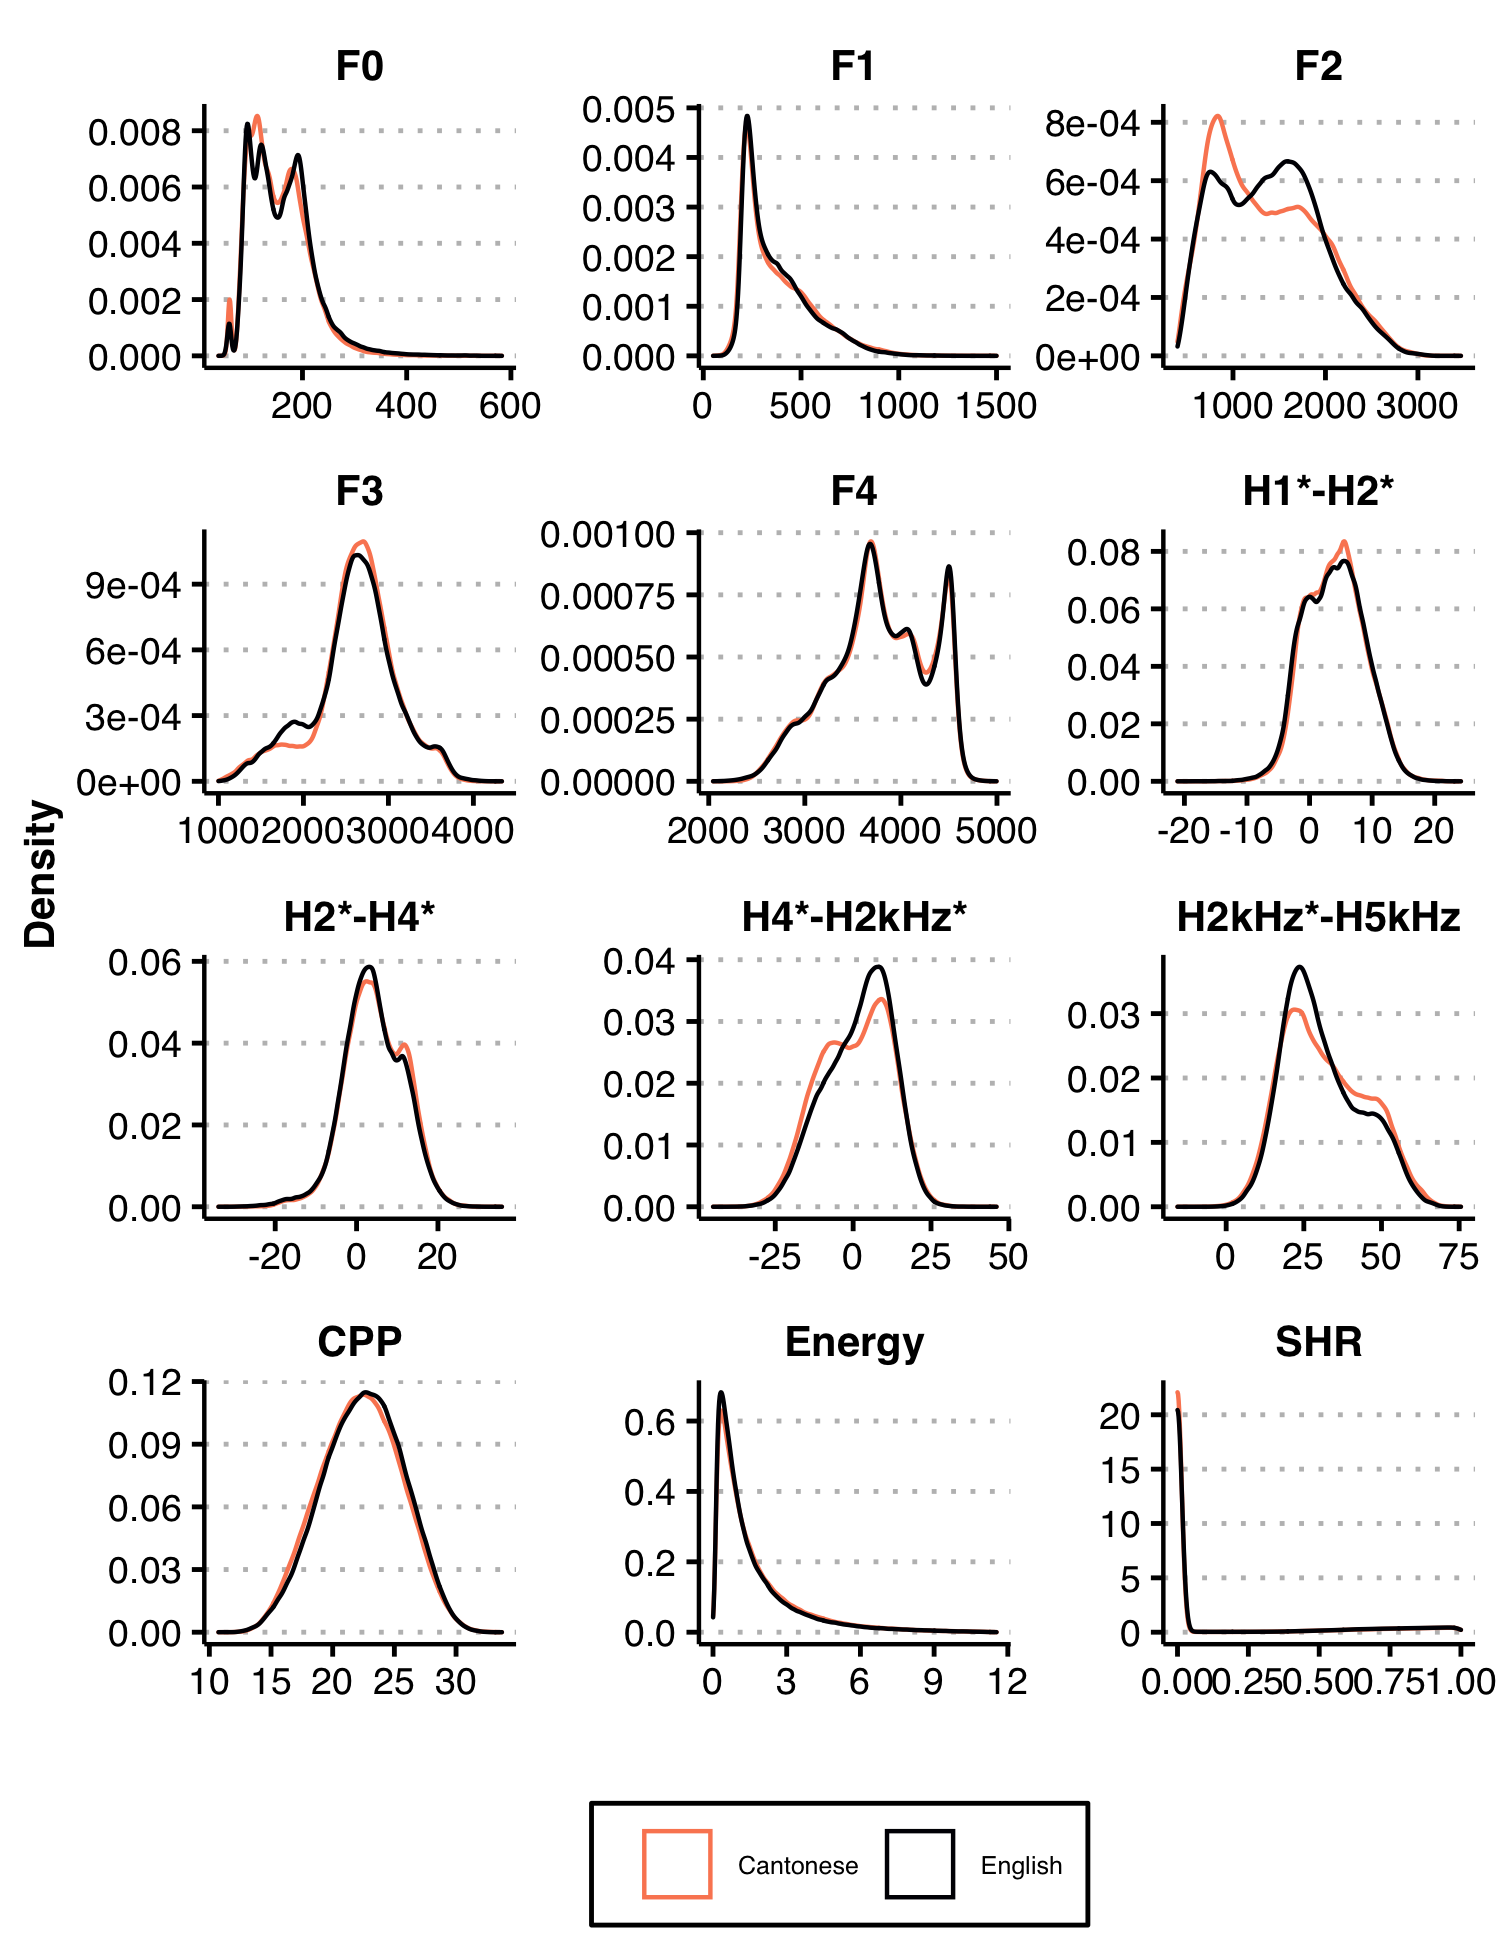
\includegraphics[width=\linewidth]{figures/ch3_allmeasuresdensity_5in.png} 
    \caption{Distribution of all acoustic measures by language after filtering.}
    \label{ch3:fig:allmeasures}
    \end{center}
\end{figure}

For each of the 12 acoustic measurements (but not the moving standard deviations), a separate Bayesian mixed-effects model was used to compare the distribution of values by talkers across languages. The models were implemented with \textit{brms} \citep[version 2.15.0;][]{burkner_2017_brms} in R \citep[version 4.0.5;][]{r_2021}. The brms package offers a simple R-based interface for fitting Bayesian models with the Stan probabilistic programming language \citep{stan_2021}. Bayesian models provide many advantages for scientific inference...\hl{ADD GENERAL METHODS MOTIVATION HERE}. For a more thorough discussion of Bayesian modeling in the phonetic sciences, please refer to the recent tutorial in \citet{vasishth_2018_bayesian}. 

A linear mixed-effects model was used for each standardized acoustic measure, with a Student's t distributed dependent variable. This decision was motivated by the strong possibility that outliers---real or erroneous---remained in the data. It also follows from Kruschke's (2013) paper arguing that robust Bayesian estimation provides better group comparison estimates. The exception to this was for SHR. As SHR is bounded by zero and one and contains many real and meaningful zero measurements, SHR was modeled as zero-inflated beta distribution. Apart from this, the models share structure and specifications. In all cases, the formula in \ref{ch3:num:formula} was used, where Measure refers to the particular acoustic measure for the model. All measures were standardized prior to modeling (except SHR). \hl{After standardization, 500 samples from each talker/language pair were randomly selected for modeling. This was done for feasibility of running.}
    
    \begin{equation}\label{ch3:num:formula}
        \text{Measure} \sim 0 + \text{Language} + (0 + \text{Language }|\text{ Talker})
    \end{equation}
    
Weakly informative priors were used in all models, following guidelines in the Stan documentation \citep{gelman_2020_prior} and from \citet{mcelreath_2020_sr}. For the the non-SHR models, these were as follows.... 

Each model consisted of four chains with 2000 iterations, half of which were warm-up iterations, for a total of 4000 samples after warm-up. \hl{ Divergent transitions, R-hat, ESS }
    
These models give high-level insight into how much individuals differed for particular acoustic dimensions across language. The models also give insight into whether or not there is a common pattern across talkers. While this part of the analysis extends the work done primarily on F0 \citep[e.g., by][]{} to the present data set, it does not elucidate how the different acoustic dimensions vary. 
    
Inference in Bayesian statistics is based on the posterior distributions, which reflect the range and probability of credible values for parameters. The comparison of interest here is the difference between the two languages for each talker. 

Figure XX depicts the magnitude of the difference across languages for CPP. \hl{describe ... the blue shaded interval depicts the recommended region of practical equivalence (ROPE) for standardized variables} \citep{kruschke_2011_rope}. Most of the comparisons overlap with the ROPE, suggesting that there is no difference in CPP across languages. Further, in the talkers with a differce, the direction is not consistent across languages. \hl{As CPP is associated with non-modal phonation types...}


\begin{figure}[htbp]
    \begin{center}
    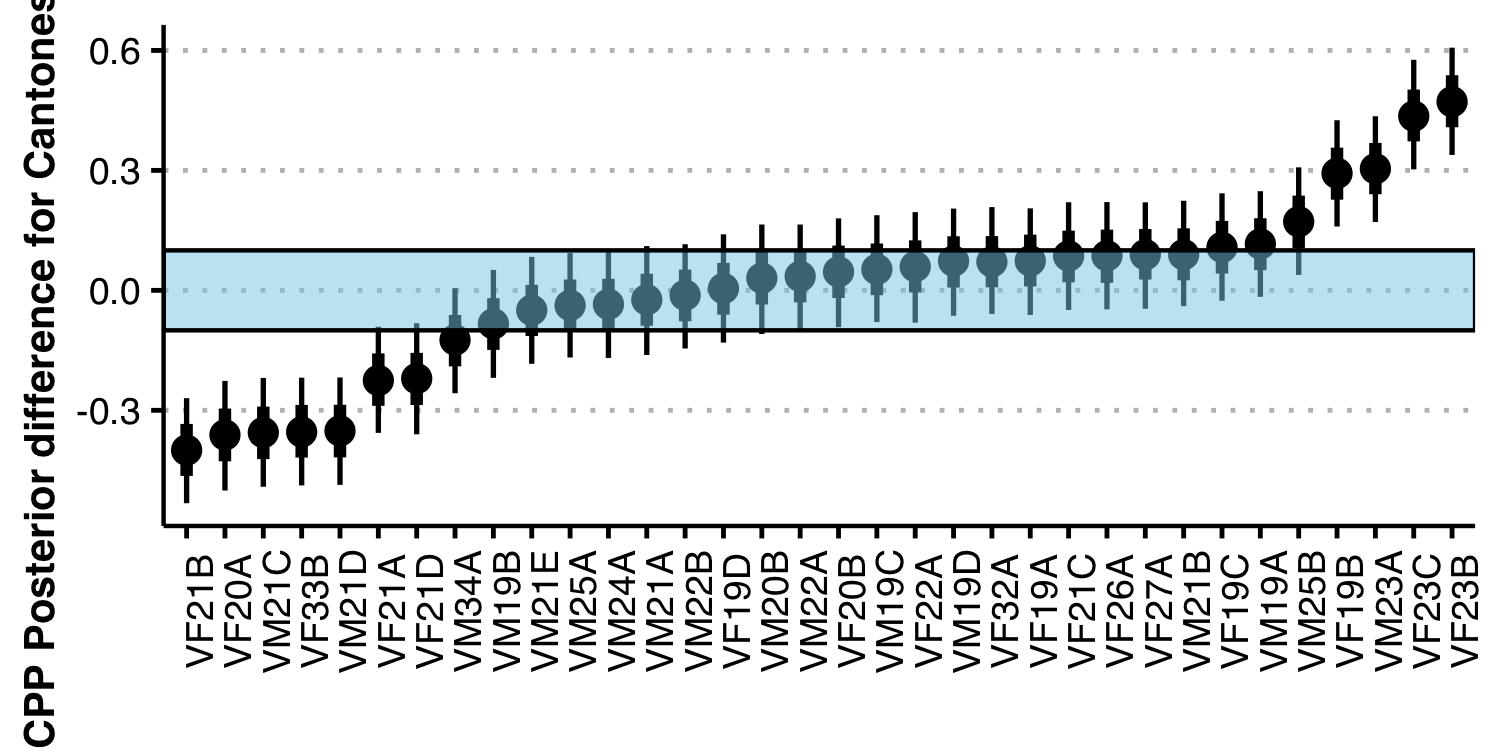
\includegraphics[width=\linewidth]{figures/ch3_cpp_5in.png} 
    \caption{Posterior difference between languages for CPP.}
    \label{ch3:fig:cpp}
    \end{center}
\end{figure}

Other variables...

In the case of SHR... how to interpret
    


% %old version
% For each acoustic measurement and talker, I conducted a Student's \textit{t}-test and calculated Cohen's \textit{d}, in order to give a high-level assessment of whether variable means differed across the two languages. These comparisons have no bearing on how a given variable \textit{varies}. Table~\ref{ch3:tab:cohend} reports counts of talkers by effect size. Notably, across all talkers and variables, only 21.1\% yielded non-trivial Cohen's \textit{d} values. Most talkers (32/34) had at least one non-trivial comparison. The distribution of these counts is depicted in Figure~\ref{ch3:fig:ntcounts}. 

% \begin{table}[htbp]
% \caption{This table reports counts of Cohen's \textit{d} for crosslinguistic comparisons of each of the acoustic measurements by talker. Degrees of freedom ranged between 49,274--136,644 across t-tests. For most talkers and variables, the difference in means was trivial, which is reflected in that column's high counts.}
% \label{ch3:tab:cohend}
% \centering
% \begin{tabular}{lccc}
% \toprule
%          & \multicolumn{3}{c}{\textbf{Cohen's \textit{d}}} \\
%          & \textbf{Trivial} & \textbf{Small} & \textbf{Medium} \\
% \textbf{Variable} & \textbf{\textit{0.0--0.2}} & \textbf{\textit{0.2--0.5}} & \textbf{\textit{0.5--0.8}} \\ 
% \midrule
% F0 & 21 & 10 & 3 \\
% F0 s.d. & 34 & 0 & 0 \\
% F1 & 24 & 9 & 1 \\
% F1 s.d. & 29 & 5 & 0 \\
% F2 & 26 & 8 & 0 \\
% F2 s.d. & 32 & 2 & 0 \\
% F3 & 24 & 9 & 1 \\
% F3 s.d. & 29 & 5 & 0 \\
% F4 & 30 & 3 & 1 \\
% F4 s.d. & 28 & 6 & 0 \\
% H1*--H2* & 18 & 15 & 1 \\
% H1*--H2* s.d. & 32 & 2 & 0 \\
% H2*--H4* & 25 & 9 & 0 \\
% H2*--H4* s.d. & 31 & 3 & 0 \\
% H4*--2kHz* & 25 & 8 & 1 \\
% H4*--2kHz* s.d. & 34 & 0 & 0 \\
% H2kHz*--5kHz* & 23 & 10 & 1 \\
% H2kHz*--5kHz* s.d. & 31 & 3 & 0 \\
% CPP & 21 & 10 & 3 \\
% CPP s.d. & 32 & 2 & 0 \\
% Energy & 17 & 14 & 3 \\
% Energy s.d. & 18 & 16 & 0 \\
% SHR & 31 & 3 & 0 \\
% SHR s.d. & 29 & 5 & 0 \\
% \bottomrule
% \end{tabular}
% \end{table}

% \begin{figure}[htbp]
% \begin{center}
% 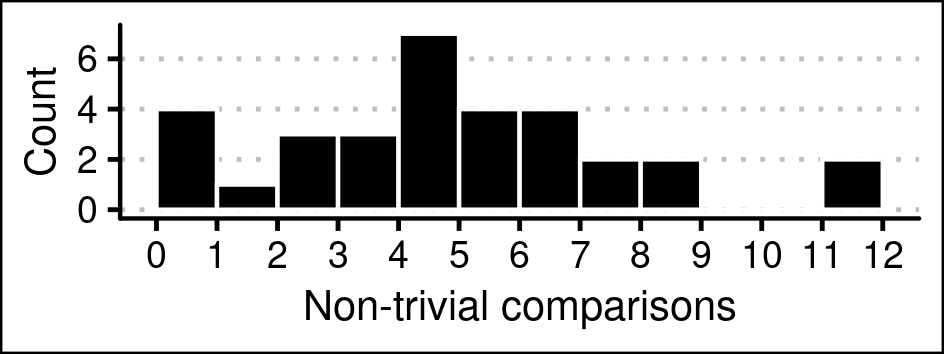
\includegraphics[width=0.875\linewidth]{figures/3-non-trivial_counts_by_talker.png} 
% \caption{A summary of the number of non-trivial comparisons from Table~\ref{ch3:tab:cohend} across the 34 talkers.}
% \label{ch3:fig:ntcounts}
% \end{center}
% \end{figure}

% For the non-trivial comparisons, there were consistent patterns across languages for H1*--H2* and F0. For the remaining variables, while some talkers exhibited a difference in mean values, the direction of the difference varied, or relatively few talkers exhibited the difference. 

% H1*--H2* was significantly higher in Cantonese for a relatively large subset of the talkers (13/34), lower for a small number (3/34), but trivial for most (18/34). While based on a different measure than \citep{ng_2012_ltas}, this is consistent with the finding that Cantonese tends to be breathier, or English creakier---the current analysis does not distinguish between these interpretations.

% If there was a non-trivial difference in F0 across languages, then Cantonese had a lower mean F0 than English (13/34; Female = 7), though most talkers did not exhibit a difference (21/34). This is consistent with prior findings that when a difference between English and Cantonese was found, Cantonese had a lower mean F0 for females \citep{ng_2012_ltas,altenberg_2006_f0}. I also observe this difference for a small number of males. 


\subsection{Principal components analysis}\label{ch3:sec:pca}
\subsubsection{Methods}
Principal components analysis (PCA) is a dimensionality reduction technique appropriate for data with many potentially correlated variables. In the case of voices, distilling numerous acoustic dimensions into a smaller number of components facilitates identifying and describing the structure of voice variability. PCA provides insight into how variables pattern together in a data set. This feature of PCA is especially relevant here, as voice perception research has made it clear that individual acoustic measurements may be necessary to capture and encode a voice but not be perceptually meaningful to listeners. What matters is how the different aspects conspire together to form a percept. 

Often, the goal of PCA is to take a large number of dimensions and extract a much smaller set to use for some additional purpose, such as regression modeling. The focus in this chapter is on the internal structure of the components. That is, I examine what makes up components for different talkers and whether an individual's voice structure varies (or not) across languages.  

I adapt methods from work on voices \citep{lee_2019_acoustic,lee_2020_language} and faces \citep{burton_2016_faces,turk_1991_eigenfaces}. The  of this analysis is to the capture similarities or differences in the structure of each talker's voice across languages. As such, I conducted PCAs separately for each talker-language pair, and compared the results of each talker's English and Cantonese PCAs. All 24 measures were normalized (z-scored) on by-PCA basis prior to the analysis. PCAs were implemented with the \textit{parameters} package \citep{makowski_2019_parameters} in R \citep{r_2021}, using an oblique \textit{promax} rotation to simplify the factor structure, as the measurements reported in the previous section were expected to be somewhat correlated given prior findings \citep{lee_2019_acoustic}, and a broader understanding of how different acoustic measures align with one another \citep{kreiman_2014_theory, kreiman_2021_validating}.

Each PCA included the number of components for which all resulting eigenvalues were greater than 0.7 times the mean eigenvalue, following \citeauthor{jolliffe_2002_pca}'s \citeyearpar{jolliffe_2002_pca} recommended adjustment to the Kaiser-Guttman rule. I used this rule, rather than a more sophisticated test (e.g., broken sticks), as it is not detrimental to this exploratory analysis to err on the side of including marginal components. Additionally, across each of the components, only loadings with an absolute value of 0.45 or higher were interpreted \citep{lee_2019_acoustic, tabachnick_2013_statistics}. While \citet{lee_2019_acoustic} use a threshold of 0.32, \citet{tabachnick_2013_statistics} note that higher loadings indicate that a particular variable is a better measure of the component, with 0.32 corresponding to poor (but still interpretable) overlap between the varialbe and the component. By the same scale, a loading of 0.45 corresponds to fair, 0.55 to good, 0.63 to very good, and 0.71 and above to excellent. Given the large number of components and loadings, in this analysis, only loadings in excess of the fair threshold are interpreted.\footnote{The Interspeech publication this chapter is expanded from used the 0.32 threshold.} 
% this section revised

\subsection{PCA results}\label{ch3:sec:pca_results} 
The PCAs across both languages for all 34 talkers resulted in 10--14 components and accounted for 74.9--82.7\% of the total variation. Half of talkers had the same number of components for each of their languages (17 of 34). Of the remainder, 16 of the 34 talkers had a difference of one in the number components, and only one had a difference of two. Talkers had 4--11 identical component configurations across their languages (M$=$7.82). These shared components represent 33.3\%--91.7\% of the total components for talkers (M$=$66.7\%). The numbers comprising these summary statistics are provided in Table \ref{ch3:tab:componentcount}. While this already indicates a substantial amount of shared lower dimensional structure across languages, it likely underestimates the actual shared structure, given that similarity of component structure is not taken into account (i.e., a component of F2, F3 and F4 versus a component with just F2 and F3), as is the case in Seciton \ref{ch3:sec:cca}. %this paragraph updated

\begin{table}[htbp]
    \caption{}
\label{ch3:tab:componentcount}
\centering
    \begin{tabular}{llllll}
    \toprule
     & \multicolumn{2}{l}{\textbf{Cantonese}} & \multicolumn{2}{l}{\textbf{English}} & \textbf{} \\
    \textbf{Talker} & \textbf{N} & \textbf{Variance} & \textbf{N} & \textbf{Variance} & \textbf{Identical N} \\
    \midrule
    \textbf{VF19A} & 11 & 0.77 & 12 & 0.80 & 8 \\
    \textbf{VF19B} & 12 & 0.78 & 12 & 0.78 & 8 \\
    \textbf{VF19C} & 12 & 0.78 & 12 & 0.79 & 9 \\
    \textbf{VF19D} & 13 & 0.81 & 13 & 0.78 & 9 \\
    \textbf{VF20A} & 11 & 0.78 & 12 & 0.79 & 6 \\
    \textbf{VF20B} & 13 & 0.81 & 12 & 0.82 & 8 \\
    \textbf{VF21A} & 12 & 0.78 & 12 & 0.80 & 6 \\
    \textbf{VF21B} & 12 & 0.78 & 12 & 0.80 & 8 \\
    \textbf{VF21C} & 14 & 0.83 & 13 & 0.83 & 10 \\
    \textbf{VF21D} & 12 & 0.79 & 12 & 0.81 & 9 \\
    \textbf{VF22A} & 11 & 0.78 & 12 & 0.80 & 7 \\
    \textbf{VF23B} & 12 & 0.78 & 12 & 0.78 & 8 \\
    \textbf{VF23C} & 12 & 0.79 & 12 & 0.80 & 7 \\
    \textbf{VF26A} & 12 & 0.78 & 13 & 0.80 & 7 \\
    \textbf{VF27A} & 11 & 0.79 & 11 & 0.77 & 8 \\
    \textbf{VF32A} & 12 & 0.78 & 11 & 0.76 & 8 \\
    \textbf{VF33B} & 12 & 0.77 & 12 & 0.79 & 9 \\
    \textbf{VM19A} & 12 & 0.78 & 11 & 0.76 & 5 \\
    \textbf{VM19B} & 11 & 0.80 & 12 & 0.80 & 6 \\
    \textbf{VM19C} & 11 & 0.76 & 11 & 0.78 & 6 \\
    \textbf{VM19D} & 13 & 0.80 & 14 & 0.82 & 10 \\
    \textbf{VM20B} & 12 & 0.80 & 11 & 0.76 & 9 \\
    \textbf{VM21A} & 10 & 0.78 & 11 & 0.79 & 5 \\
    \textbf{VM21B} & 11 & 0.79 & 11 & 0.76 & 9 \\
    \textbf{VM21C} & 12 & 0.80 & 12 & 0.77 & 9 \\
    \textbf{VM21D} & 11 & 0.75 & 12 & 0.77 & 7 \\
    \textbf{VM21E} & 10 & 0.74 & 12 & 0.80 & 7 \\
    \textbf{VM22A} & 12 & 0.77 & 13 & 0.83 & 11 \\
    \textbf{VM22B} & 12 & 0.79 & 12 & 0.79 & 7 \\
    \textbf{VM23A} & 12 & 0.81 & 12 & 0.79 & 4 \\
    \textbf{VM24A} & 11 & 0.77 & 11 & 0.76 & 8 \\
    \textbf{VM25A} & 12 & 0.81 & 12 & 0.77 & 11 \\
    \textbf{VM25B} & 11 & 0.74 & 12 & 0.76 & 7 \\
    \textbf{VM34A} & 11 & 0.77 & 12 & 0.81 & 10 \\
    \bottomrule
    \end{tabular}
\end{table}

To assess whether talkers exhibit the same structure in voice variability across their languages, I first consider the patterns present across the different PCAs, as this provides context for understating what unique structural characteristics in talkers' voices looks like. To this end, I briefly summarize common patterns across PCA components, regardless of how much variance they account for, as the difference is often quite small. Figure~\ref{ch3:fig:VF32A} shows the first four components of a single talker's Cantonese and English PCAs, illustrating some examples of how components can vary (or not) across languages. It also highlights the importance of not attributing too much value to the ordering of components, but rather to their composition and variance accounted for.

\begin{figure}[htbp]
\begin{center}
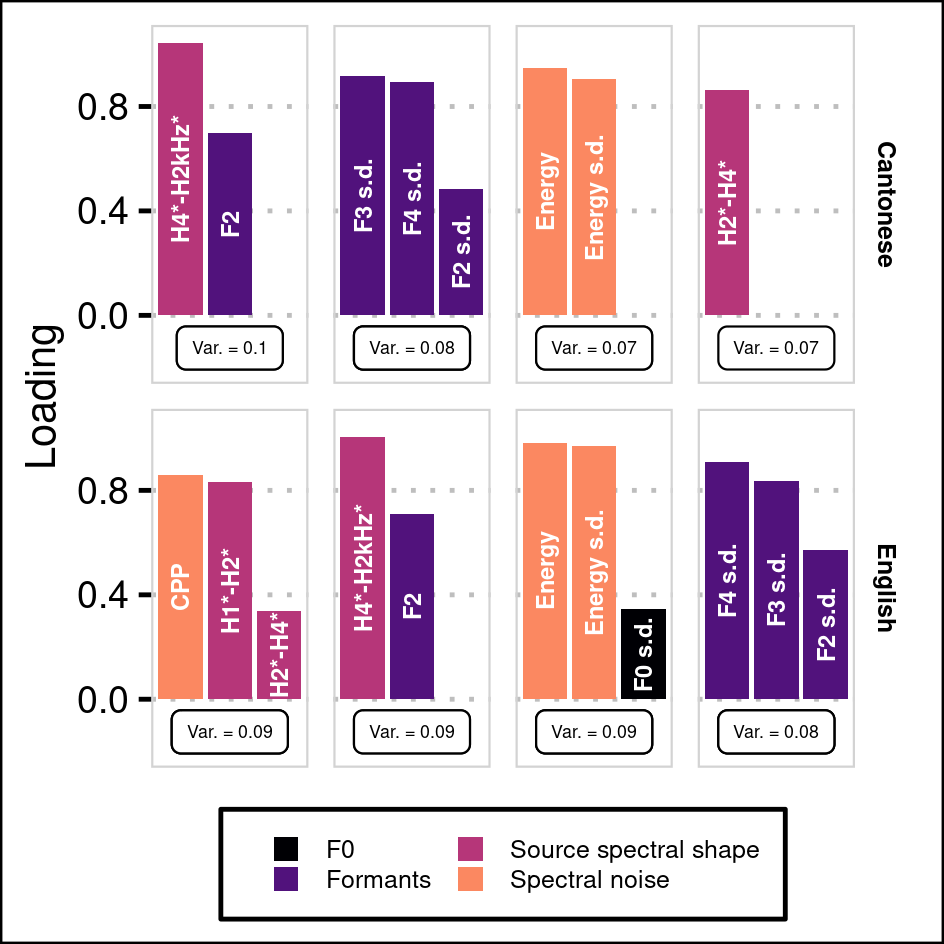
\includegraphics[width=0.875\linewidth]{figures/3-VF32A_pretty.png} 
\caption{In the first four components of a talker's Cantonese and English PCAs, loadings are represented by bar height and are labelled with the variable name; color represents conceptual groupings; and, the component's variance is superimposed.}
\label{ch3:fig:VF32A}
\end{center}
\end{figure}

Broadly speaking, there were a lot of similarities in component composition across both talkers and languages. The following paragraphs summarize the components that were present in every PCA, regardless of talker or language. This is followed by a summary of the variables with the least consistent pattern across components. 

The shared component accounting for the most variation across talkers had a core structure consisting of F2 and H4*-H2kHz. These usually went along with H2kHz*-H5kHz* (Cantonese = 34, English = 31), and occasionally with F3 and F4 (Cantonese = 3, English = 3). In a similar vein, all talkers had a component consisting of H4*-H2kHz* s.d. and H2kHz*--H5kHz* s.d., though it accounted for a smaller proportion of the total variation. \hl{Describe what these mean}

While F3 and F4 often patterned with the higher spectral tilt paramters, they were more liekly to cooccur with just each other (Cantonese = 28, English = 26)

Formant s.d. pattern

Spectral tilt s.d. pattern 

The spectral noise parameters had relatively consistent component patterns across talkers and languages. Energy and Energy s.d. consistenly loaded on the same component, and were sometimes accompanied by F0 (Cantonese = 6, English = 2) and F0 s.d. (Cantonese = 1). CPP s.d. occurred consistently on its own component for all English PCAs, and 31 of the Cantonese PCAs. In the remaining three cases, it was accompanied by CPP (n=1) or H1*-H2* s.d. (n=2). CPP patterned less consistently, but was most often accompanied by F0 s.d. (Cantonse = 19, English = 14). SHR and SHR s.d. exclusively loaded together for 31 talkers in each language, and SHR by itself for a single talker per language. The pair was sometimes accompanied by H1*-H2* (Cantonese = 2, English = 2), H2*-H4* (English = 1), or F0 (English = 3). \hl{Describe what these mean}


While this covers a lot of the variables included in the PCAs, F0 is notably sparse in the above paragraphs. This is because F0 patterned very inconsistently.



% , with the eight most commonly occurring components summarized in Table~\ref{ch3:tab:components}. For context, recall that PCAs had anywhere from 10--14 components total. These eight components consisted of source spectral shape, spectral noise, as well as formant variables. On the other hand, F0 co-occurred with a wide variety of variables (often Energy), but in a manner that was less consistent across talkers. There were additional components (not reported here) that were shared by less than half of talkers. In summary, despite the greater amount of shared structure across PCAs than found in \citet{lee_2019_acoustic}, there is still ample room for idiosyncratic variation, both in terms of which variables co-occur, as well as in how much variance different components account for. 

% \begin{table}[th]
% \caption{A summary of the most commonly occurring components across all PCAs. Variables are only included if $|$Loading$|>$ 0.32. Italics indicate additional variables that were present on a component for a subset of talkers (i.e., an alternative but related configuration). \textit{N} indicates the number of times a component occurred (out of 34), and \textit{Var. \%} gives the range of percent variance accounted for by the component.}
% \label{ch3:tab:components}
% \centering
% \begin{tabular}{lcccc}
% \toprule
%  & \multicolumn{2}{c}{\textbf{Cantonese}} & \multicolumn{2}{c}{\textbf{English}} \\
% \textbf{Variables} & \textbf{N}  & \textbf{Var. \%}  & \textbf{N}  & \textbf{Var. \%} \\
% \midrule
% \begin{tabular}[c]{@{}l@{}}H4*--H2kHz*,\\ H2kHz*--H5kHz*, F2, \\\textit{F3}, \textit{F4}\end{tabular} & 34 & 9.3--15.5 & 32 & 9.2--16.7 \\
% \midrule
% \begin{tabular}[c]{@{}l@{}}H4*--H2kHz* s.d.,\\ H2kHz*--H5kHz* s.d.\end{tabular} & 32 & 6.3--8.3  & 34 & 4.1--5.0  \\
% \midrule
% \begin{tabular}[c]{@{}l@{}}Energy, Energy s.d, \textit{F0}\end{tabular} & 31 & 5.8--9.4  & 33 & 6.3--9.1  \\
% \midrule
% CPP s.d. & 29 & 4.1--5.0  & 31 & 4.1--4.9  \\
% \midrule
% \begin{tabular}[c]{@{}l@{}}SHR, SHR s.d.\end{tabular} & 30 & 3.8--7.5  & 29 & 5.4--7.3  \\
% \midrule
% \begin{tabular}[c]{@{}l@{}}F3, F4, \textit{F2}\end{tabular} & 26 & 6.0--8.5  & 29 & 5.8--8.5  \\
% \midrule
% \begin{tabular}[c]{@{}l@{}}F3 s.d., F4 s.d., \textit{F2 s.d.}\end{tabular} & 26 & 5.3--8.6  & 29 & 4.7--8.6  \\
% \midrule
% \begin{tabular}[c]{@{}l@{}}H2*--H4* s.d., \\H1*--H2* s.d.\end{tabular} & 26 & 4.2--6.5  & 28 & 4.2--6.8  \\
% \bottomrule
% \end{tabular}
% \end{table}


\subsection{Canonical redundancy analysis}\label{ch3:sec:cca}
\subsubsection{Methods}
In order to assess whether variation in a talker's voice is structurally similar across both languages, I compare PCA output from both languages by calculating redundancy indices in a canonical correlation analysis \citep[CCA][]{stewart_1968_canonical, jolliffe_2002_pca}.  CCA is a statistical method used to explore how groups of variables are related to one another. The two sets of variables are transformed such that the correlation between the rotated versions is maximized. This is useful here, as a talker may have similar components in their English PCA and Cantonese PCA, but these components might not necessarily be in the same order, even if they account for comparable amounts of variance.

Redundancy is a relatively simple way to characterize the relationship between the loadings matrices of two PCAs---the two sets of variables under consideration here. For example, the two indices represent the amount of variation in a talker's Cantonese PCA output that can be accounted for via canonical variates by their English PCA output, and vice versa. Notably, the two redundancy indices are not symmetrical \citep{stewart_1968_canonical}. This is particularly relevant in cases where the PCAs comprise different numbers of components, as determined by the stopping rule described above.

I computed redundancy indices for all pairwise combinations, including cases where similar values were expected (same talker, different language), and cases where I expected dissimilarity (different talker and language). Considering that the PCA analyses retain the lower-dimensional structure within each language, these redundancy indices effectively reflect the degree to which the lower-dimensional structure of the voice variability is retained across a talker's two languages.

\subsubsection{Results}


Redundancy indices for within-talker comparisons ranged from 0.82 to 0.99, (\textit{Mdn} = 0.93, \textit{M} = 0.92, \textit{SD} = 0.04), and are displayed in Figure~\ref{ch3:fig:redundancy}, with the two redundancy indices for a given pair plotted against one another. Comparisons across talkers within-language (range: 0.63--0.98, \textit{Mdn} = 0.84, \textit{M} = 0.84, \textit{SD} = 0.6) and across-language (range: 0.66--0.98, \textit{Mdn} = 0.83, \textit{M} = 0.84, \textit{SD} = 0.6) are generally lower, but still relatively high. Within-talker values were confirmed to be higher than across-talker comparisons [\textit{Welch's t}(71.36) = --17.83, \textit{p} $<$ 0.001, d = 1.76]. 

The high values are not unexpected. As PCA is a dimensionality reduction technique, the discarded components almost certainly contain idiosyncratic variation. Moreover, and following from Section~\ref{ch3:sec:pca_results}, there were a substantial number of commonly occurring patterns across talkers and languages. 

\begin{figure}[htbp]
\begin{center}
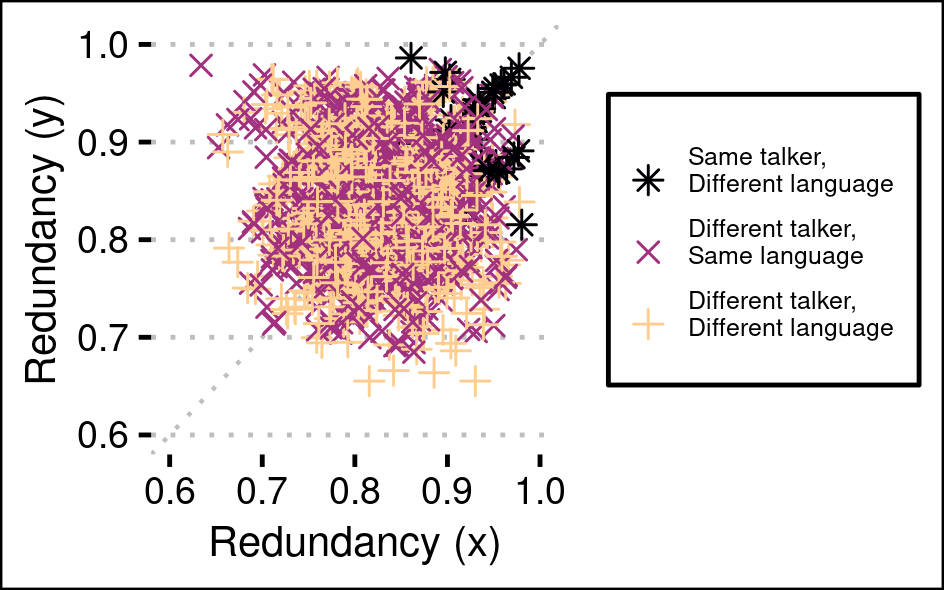
\includegraphics[width=0.875\linewidth]{figures/3-reds_pretty.png} 
\caption{The relationship between the two redundancy indices for three different types of comparisons. Within-talker comparisons are clustered at the top right.}
\label{ch3:fig:redundancy}
\end{center}
\end{figure}


\section{Passage length analysis}\label{ch3:sec:passagelength}



\section{Discussion and conclusion}\label{ch3:sec:discussion}

This study examines spectral properties and structural similarities in an individual's voice in two languages. A clear result is that most of the bilinguals studied here exhibit similar spectral properties, and similar lower-dimensional structure in voice variation, despite substantial segmental and suprasegmental differences across English and Cantonese \citep{matthews_2013_cantonese}. In this sense, a majority appear to have the same ``voice'' across languages, which renders voice-as-an-auditory-face an apt comparison.

The comparison of these 34 Cantonese-English bilinguals' voices across languages suggest more similarity for an individual across languages than found within a more tightly controlled group of monolingual English speakers \citep{lee_2019_acoustic}---several analysis decisions may have contributed to this. I compared similar components independent of order, which ignores the fact that similar components may account for different amounts of variance, but ensures that any comparisons made are among like items. Any downside to this methodological decision is mitigated by the fact that most components made relatively small contributions, accounting for 4.2--10.3\% (95\% highest density interval) of the PCA's total variance. 

While statistical choices may have affected these results, the data differences between the current and previous studies are also important to note. This study uses substantially longer passages than the short samples in \citet{lee_2019_acoustic}. The larger speech sample may allow for a more stable underlying structure to showcase itself, as opposed to the potential for ephemeral variation in a shorter sample. This possibility is easily testable by manipulating the length of the speech sample in the analysis.

Ultimately, the goal is to understand how the acoustic variability and structure of talkers' voices maps onto listeners' organization of a voice space for use in talker recognition and discrimination. Turning to listener and behavioural data will help in deciphering what is meaningful variation within a voice from low level noise that cannot be attributed to a particular vocal signature. Verification from listener performance will help adjudicate which statistical choices present an acoustic voice space that matches listener organization. 

\endinput % -------------------------------------------------------- %

%%!TEX root = dissertation.tex
\setcounter{chapter}{3}

\chapter{The structure of voice onset time variation in bilingual long-lag stop categories}\label{Uniformity}

\section{Introduction}\label{ch4:sec:intro}

A consequence of bilingualism is that individuals must navigate segment inventories that exist in a shared phonetic space, in which categories may or may not share aspects of their mental representations \citep{flege_2021_slmr}. One of the primary goals in this chapter is to address what languages share, if anything, in the mental representation of speech sound categories. The idea of representation is intended here in the manner typically meant by psycholinguists \citep[e.g.,][]{llompart_2018_acoustic}, exemplar theory proponents \citep[e.g.,][]{amengual_2018_laterals}, and \citet{flege_2021_slmr} in the revised Speech Learning Model (SLM-r). \citeauthor{flege_2021_slmr} describe the units of a multilingual segment inventory as categories comprising input distributions of exemplars: ``the sensory stimulation associated with...speech sounds that are heard and seen during production by others...in meaningful conversations'' \citep[][p. 32]{flege_2021_slmr}. So, if sound categories from different languages exist in the same phonetic space and are represented by distributions of exemplars, how, then, can the extent to which languages share representation(s) be assessed? Much like Chapter \ref{ch3:Voice}, the approach here is one of elucidating the structure of variation. 

There are many pieces to this puzzle, and the literature has already addressed some of them. The introduction to this chapter proceeds as follows---section \ref{ch4:sec:links} addresses which sound categories are candidates for shared representation in the first place. Section \ref{ch4:sec:cli} briefly summarizes the relevant crosslinguistic influence literature, addressing assimilation, dissimilation, and how they reflect on the idea of shared representation. Section \ref{ch4:sec:uniformity} identifies a limitation of the existing paradigms in crosslinguistic influence and proposes adapting the uniformity framework as a way to fill the gap. This framework offers a way to interpret the structure of variation for a given acoustic dimension. Section \ref{ch4:sec:rqs} introduces the focus of this particular study---long-lag stops in Cantonese and English---and outlines the specific research questions and hypotheses.

\subsection{Identifying ``links'' across languages}\label{ch4:sec:links}

At first glance, the best candidates for shared representation are sound categories discussed as being ``linked'' together. Yet, the definition of links can be frustratingly vague in the multilingualism literature. In a handbook chapter on bilingual phonetics and phonology, \citet{simonet_2016_bilingualism} describes ``links or connections of one sort or another between the phonetic categories'' (p. 10). While vague, links nonetheless represent a crucial concept. In the most basic sense, links are defined by the behavior they account for---they exist between sound categories that exert influence on one another under some set of circumstances. Links behave dynamically, as as such,  \citeauthor{simonet_2016_bilingualism} also notes that ``these connections...are transiently strengthened in contexts that induce the activation of both languages and inhibited in contexts that favor the use of only one of the languages'' \citeyearpar[][p. 10]{simonet_2016_bilingualism}. Arguably, the links must exist because crosslinguistic influence can be observed. While there may be alternative explanations (i.e., global influence), the concept of links is widely used in accounting for bilinguals' behavior. 

\citet{flege_2021_slmr} expand on links in the SLM-r, providing a framework for predicting which sound categories will be linked together. The proposal is simple---namely, sound categories will be linked to the closest category in the other language. Determining which categories pair up, however, remains an empirical challenge from the perspective of speech production, and as a result, \citet{flege_2021_slmr} rely on perceptual metrics. The reason for this challenge is because perception and production do not always line up neatly. \citeauthor{flege_2021_slmr} assert that similarity ``must be assessed perceptually rather than acoustically because acoustic measures sometimes diverge from what listeners perceive'' \citeyearpar[][p. 33]{flege_2021_slmr}. This assertion is echoed in an overview chapter on crosslinguistic segment similarity, where \citet{chang_2015_similarity} argues that in accounting for behavior, similarity is best captured abstractly. \citeauthor{chang_2015_similarity} states that crosslinguistic influence at the segmental level tends to occur between sounds that share ``(1) similar positions in the respective phonemic inventories (when considering the contrastive feature oppositions---or, more broadly, the `relative phonetics'---of the sounds in relation to other sounds in the inventory), and (2) similar distributional facts'' \citeyearpar[][p. 201]{chang_2015_similarity}. This approach to similarity emphasizes a general role for abstraction but does not necessarily invite a formal phonological analysis. Developing such an analysis would likely constitute a dissertation in itself---\citet{mielke_2012_similarity} highlights the challenges of applying phonological features across languages, given the sheer variety of phonetics-phonology mappings in the world's languages. 

While \citet{flege_2021_slmr} and \citet{chang_2015_similarity} take different approaches, perceptual ratings and relative phonetics accomplish a similar goal---they account for abstraction and nonlinearity in listeners' mental representations. In sum, abstract similarity seems to be a prerequisite for the emergence of a link between two sound categories, given how it does a better job of accounting for when and where crosslinguistic influence occurs. The presence of abstract similarity, however, does not address what happens next. It does not entail any particular outcome, and it does not directly address how representation is structured for the sound categories in question. 

\subsection{Crosslinguistic influence and representation}\label{ch4:sec:cli}

The next step in the puzzle is understanding what happens to linked sound categories. The SLM-r outlines two primary outcomes for sound categories in a shared system---assimilation and dissimilation \citep{flege_2021_slmr}. Assimilation is a merging of phonetic properties and arguably occurs when bilinguals and learners do not perceive a difference between two categories. Dissimilation, then, is the reverse---a diverging of phonetic properties that occurs when a difference is perceived. Notably, these processes need not impact all phonetic properties in the same way. For example, in a study of coronal stops produced by simultaneous French-English bilinguals, \citet{sundara_2006_production} found that bilinguals differentiated languages on voice onset time (VOT) and the standard deviation of burst frequency but not on the other spectral moments that monolinguals did differentiate. This study illustrates convergence on some but not all properties. 

The motivation for these outcomes arises from two simple constraints from the productive and perceptual systems. Effectively, don't get too close to each other in perception, and don't get too complicated in production \citep{guion_2003_systems, lindblom_1988_universals, flege_2021_slmr}. These constraints lead SLM-r to posit that proximity leads to instability, even if what counts as close remains unclear, and that the outcome of instability is assimilation and dissimilation. Considering how bilinguals are fully capable of maintaining subtle distinctions for similar sound categories across languages \citep[e.g.,][]{sundara_2006_production, lein_2016_vot, casillas_2021_interlingual}, this is not a trivial point to make. It may thus be more appropriate in the case of early bilinguals to also consider contrast maintenance alongside dissimilation. 

By following what SLM-r posits, a relatively simple account is that dissimilation for similar sound categories would lead to distinct representations of those categories. A similarly straightforward account is that assimilation leads to a shared representation. The picture is complicated, however, by the idea of imperfect assimilation and what \citeauthor{flege_2021_slmr} term \textit{composite categories}. In the SLM-r, if sounds from two languages are phonetically too close to each other, they will remain linked in a composite category "defined by the statistical regularities present in the combined distributions of the perceptually linked...sounds." \citep[][p. 41]{flege_2021_slmr}. This scenario might be characterized as imperfect or partially shared representation, where certain dimensions are kept apart and others overlap. For example, the place of articulation may be shared across languages even if VOT differs. Alternatively, this lack of clear-cut examples of assimilation in the literature may instead indicate that assimilation and dissimilation might be better cast as ends of a spectrum for a gradient, context-sensitive phenomenon. This re-conceptualization makes room for things like contrast maintenance and composite categories.

There are a few potential reasons for the lack of clear-cut assimilation. First, true assimilation might just be rare in bilingual speech. This reason is supported by a recent meta-analysis of crosslinguistic influence for Spanish and English initial stop consonants \citep{casillas_2021_interlingual}. In this environment, English long-lag stops and Spanish short-lag stops are linked to one another \citep{fricke_2016_phonetic, goldrick_2014_switching, bullock_2009_sociophonetics, olson_2016_transfer}. \citeauthor{casillas_2021_interlingual} found that early bilinguals did not produce ``compromise'' stop categories. That is, early Spanish-English bilinguals did not produce VOT was somehow intermediate to canonical productions by monolinguals of either language. Instead, the production of each category was influenced by task demands and factors such as social context. So while some assimilation occurs, it is far from the only process. This finding echoes arguments made by \citet{bullock_2009_sociophonetics} on the sophistication and control that bilinguals exert over their possible forms. So while there is clear evidence of a link between the two sounds, there is no compromise category. Instead, bilinguals produce a wide range of forms appropriate to and influenced by different contexts. Without considering task and context factors, it is perhaps not surprising that the two sound categories masquerade as a single composite category. 

A second reason for the rarity of complete assimilation arises from the experimental and corpus-based approaches typically used to study crosslinguistic influence. Experimental approaches to crosslinguistic influence typically use sentence reading, isolated word production, or picture naming with one of several common manipulations. At a more global scale, some studies set the language mode of the full session and compare individuals across sessions \citep{grosjean_2011_transfer, simonet_2019_convergence, sancier_1997_drift}, or compare groups of individuals in different language mode conditions \citep{antoniou_2010_context}. At a more local level, experimental designs leverage language switching across blocks \citep{sundara_2006_production}, trials \citep{goldrick_2014_switching}, or within trials \citep[i.e., prompted code-switching][]{bullock_2009_sociophonetics,antoniou_2011_VOT}. Both types of experimental studies often include both cognate and non-cognate items as a secondary manipulation \citep{}. Corpus-based approaches similarly tend to focus on proximity to code-switching \citep{fricke_2016_phonetic, balukas_2015_vot} and cognate production \citep{brown_2015_finegrained}. Across all study types, there are common findings. Typically, cognates, words occurring before a language switch, and words produced in more bilingual modes tend to show increased convergence. Conversely, unilingual modes, non-cognates, and words occurring far from a code-switch tend to show a greater degree of contrast maintenance. While there is a tendency for convergence, \citet{bullock_2009_sociophonetics} demonstrate that proximity to a code-switch leads some individuals to exaggerate the difference between English and Spanish VOT. 

In these approaches, the ability to examine crosslinguistic influence for any given pair of sounds hinges on the presence of an observable difference under some set of conditions. I posit that for this reason, most prior work in crosslinguistic influence has focused on sounds that are phonologically similar (i.e., abstract, relative phonetics) yet phonetically distinct. A common example of this arises from languages that differ in their initial stop voicing contrasts. North American English contrasts long- and short-lag stops in initial position; conversely, Spanish contrasts short-lag and prevoiced initial stops. Despite the clear difference in how the languages encode a laryngeal timing contrast, there is strong evidence for a crosslinguistic link between English long-lag and Spanish short-lag stops \citep{casillas_2021_interlingual, fricke_2016_phonetic, goldrick_2014_switching, bullock_2009_sociophonetics, olson_2016_transfer}. 

These studies demonstrate phonetic convergence---or variable assimilation---in two ways. First, VOT is shorter for English initial stops produced by bilinguals when compared to monolingual control groups. This result is attributed to the influence on English long-lag stops from the short-lag category in the other language \citep{olson_2016_transfer}. Similarly, French-English bilinguals are more likely to produce lead voicing in initial English voiced stops compared to English monolinguals \citep{sundara_2006_production}. Second, evidence of crosslinguistic influence can also come from comparing bilinguals to themselves across different circumstances. For example, \citet{fricke_2016_phonetic} use a spontaneous speech corpus to demonstrate that Spanish-English bilinguals produce shorter, more Spanish-like VOT in the lead up to an English-to-Spanish code switch \citep{fricke_2016_phonetic}. While this body of work makes the presence of a link clear, it also highlights that there are distinct aspects of how these sound categories are represented in the bilingual mind \citep{casillas_2021_interlingual}. In the SLM-r, these examples might be considered composite categories. Alternatively, they might be examples of contrasts being maintained in the face of proximity.

In any case, this focus presents a conundrum. By using methods where observing similarity hinges on the ability to detect a difference, researchers preemptively exclude the best candidates for shared representation---those that share both abstract and acoustic similarity. One example comparing highly similar sound categories in the early bilingualism literature comes from a lab-based study of Mandarin-English bilingual children \citep{yang_2019_vot}. The authors found that highly proficient bilingual 5 to 6-year-olds produced equivalent VOT for Mandarin and English long-lag stops, even though the monolingual comparison groups were consistently different. \citeauthor{yang_2019_vot}'s result suggests that the difference is either too small to maintain or that 5 to 6-year-old children have not yet mastered it. These claims should be tempered, however, as \citet{yang_2019_vot} did not control for language mode, and adult bilingual behavior was not considered. 

Despite some inroads, there is nonetheless a distinct paucity of work examining highly phonetically similar speech sounds across languages, even when such a connection would make sense. A recent study of crosslinguistic influence in Cantonese-English bilinguals compares English long-lag and Cantonese short-lag stops in the context of a language switching paradigm \citep{tsui_2019_switching}. While this comparison reflects the need for stimuli to be acoustically distinct beforehand, it glosses over the fact that both languages contrast short-lag and long-lag VOT in initial position. The best candidates for links---and accompanying crosslinguistic influence---are the long-lag stops in each language. These stops occupy the same relative position in their respective inventories and bear resemblance physically (e.g., see references in Section \ref{ch4:sec:rqs}). The null result with balanced bilinguals is thus unsurprising. I do not mean to suggest that the \citep{tsui_2019_switching} would have gotten more insightful results by comparing Cantonese long-lag stops to English long-lag stops. Instead, I aim to highlight the design constraints of the paradigms used in crosslinguistic influence research. 

Such methods are better suited for detecting links between sound categories and documenting the circumstances that undergird parallel activation of languages. In \citeauthor{grosjean_2011_transfer}'s \citeyearpar{grosjean_2011_transfer} terms, these methods are best suited to detecting \textit{interference}, as opposed to \textit{transfer}. Interference is the kind of crosslinguistic influence observed between simultaneously activated representations, while transfer occurs on a longer time scale, affecting the representations themselves. 

A good example of interference comes from Catalan-Spanish bilinguals' vowel production. \citet{simonet_2019_convergence} compare vowels on a within-talker basis from two separate sessions---unilingual Catalan and bilingual Spanish-Catalan---and found that Catalan /a/ was produced more like its Spanish counterpart in the bilingual session. While this is a straightforward result, what is unique about it, is that the authors show a dynamic within-talker process facilitated by language mode. In one setting, talkers maintain a contrast, while in the bilingual setting, they show partial assimilation. When both languages are activated, Catalan interferes with Spanish, leading to the observed outcome of phonetic convergence. \citet{simonet_2019_convergence} argue that these sounds are linked and thus simultaneously activated but ultimately have separate representations in long-term memory. In its discussion of category formation, SLM-r is more concerned with assimilation and dissimilation at the level of long-term representations \citep[i.e., transfer][]{flege_2021_slmr}. In such cases, the methods should not have to rely on the presence of detectable acoustic differences. Notably, however, transfer and interference are difficult to disentangle \citep{grosjean_2011_transfer}. 

To summarize, most work in crosslinguistic influence has focused on phonologically similar yet phonetically distinct pairs of segments and how they interfere with one another in online processing. These pairs are not strong candidates for transfer and shared mental representation (as defined at the beginning of this chapter). This widespread focus likely arises for several different reasons. The established paradigms---which facilitate research immensely---tend to require a detectable difference. It is also possible that assimilation in long-term mental representations is rare for early bilinguals, which would greatly limit the options for studying such a phenomenon. Additionally, comparisons of categories that already exhibit both abstract and phonetic similarity may be taken for granted and not considered an interesting problem to focus on, despite the nature of the mental representation of sound categories being a key focus in psycholinguistics \citep{samuel_2020_resist}. 

While many psycholinguists are indeed concerned with representation, processing has taken center stage in the psycholinguistics of bilingualism. In a prominent example of this, \citet{fricke_2019_bilingualism} argue that ``bilingualism has the potential to reveal the fundamental breadth and underlying nature of variation in language processing'' \citeyearpar[][p. 204]{fricke_2019_bilingualism}. I argue in this chapter that bilingualism also offers a window into understanding the nature of mental representation. And, in the interest of understanding it, the best category candidates would be the hardest to distinguish using surface forms in the first place. 

\subsection{Adapting the uniformity framework}\label{ch4:sec:uniformity}

The study described in this chapter focuses on assessing whether phonetically similar sounds share a mental representation or not. Unlike prior work focusing on variable convergence and divergence, this chapter addresses whether a single category deploys to both languages or whether each language carries a separate representation of similar categories. Testing directly for shared structure in this way means that the set of methods that rely on detecting and modulating differences is not appropriate. To this end, I extend the articulatory uniformity framework to the study of multilingual segment inventories. 

Articulatory uniformity is conceptualized as a constraint on within-talker phonetic variation, in which articulatory gestures or phonological primitives are implemented systematically in speech production \citep{chodroff_2017_structure, faytak_2018_uniformity, menard_2008_invariance}. The core idea of the articulatory uniformity framework is that phonetic variation is highly structured. While \citet{chodroff_2017_structure} draw tight connections between uniformity and phonological features, \citet{faytak_2018_uniformity} emphasizes how talkers learn and reuse articulatory gestures. The articulatory account builds on earlier work by \citet{menard_2008_invariance}, who argue that the stability of the first formant in French vowel production is best accounted for by stability in the tongue height gesture. While the theoretical accounts vary somewhat by author, there is nothing to suggest that such accounts are incompatible with one another. That is, both articulatory and phonological explanations are likely valid. Given the focus of this chapter on phonetic and psycholinguistic accounts of category formation and representation, the articulatory account---with its accompanying acoustic consequences---is perhaps more appropriate. 

In this light, if a set of segments share an attribute, then talkers should implement the segments with the same phonetic target or articulatory gesture---which may or may not have an acoustic consequence. This systematicity has been observed for vowel height \citep{menard_2008_invariance}, tongue shape \citep{faytak_2018_uniformity}, fricative peak frequency, and stop consonant VOT \citep{chodroff_2017_structure}. In the case of VOT in particular, the relationship between a laryngeal gesture and its acoustic consequence is clear. This allows for the extension of \citeauthor{menard_2008_invariance}'s \citeyearpar{menard_2008_invariance} argument regarding F1 and tongue height to VOT and its corresponding laryngeal gesture. Reusing the gesture across sounds that share the relevant attribute ``may simplify the somatosensory feedback needed to control the speech task`` \citep[][p. 26]{menard_2008_invariance}. In simple terms, reusing gestures is easier than the alternative in the case of high vowels. I posit that the same argument could easily be extended to long-lag stops. 

Findings for stop consonant within-language uniformity appear to be quite robust. \citet{chodroff_2017_structure} report consistent results across a lab study based on reading a list of CVC words and a corpus study comprising connected read speech. \citet{chodroff_2019_l2} replicate the uniformity findings for stop consonants with connected read speech samples from 140 non-native English speakers with a wide range of native languages in the ALLSSTAR corpus \citep{bradlow_2011_allsstar}. While \citet{chodroff_2019_l2} found a greater degree of between-talker variability with non-native speakers compared to the prior monolingual work, the within-talker structure was robust. However, the uniformity framework has not yet been extended to early bilingual speech, in particular as a mechanism for comparing how bilinguals produce phonetically similar sounds in each of their languages. Extending the framework across languages follows the framing of uniformity as arising from articulatory reuse \citep{faytak_2018_uniformity}, effectively asking whether or not reuse extends across languages. 

\subsection{Long-lag stops in Cantonese and English}\label{ch4:sec:rqs}

English and Cantonese initial long-lag stops are strong candidates for shared mental representation because they exhibit both relative and physical phonetic similarity, akin to the difference for Mandarin and English in \citet{yang_2019_vot}. Consider the initial stop [k\textsuperscript{h}]---in citation speech---with a mean VOT of 80 ms in American English \citep{lisker_1964_vot} and 91 ms in Hong Kong Cantonese \citep{clumeck_1981_cantonese}. While these values are objectively different---though based on small sample sizes---it seems that using the same laryngeal timing gesture would be advantageous given the small difference across monolingual populations that may or may not be perceptible. There is ample work documenting VOT across different varieties of English and speaking styles, with values in the 30--50 ms range in spontaneous speech \citep{stuartsmith_2015_private}. There is far less work documenting Cantonese long-lag VOT; nonetheless, descriptive work casts it as having generic long-lag aspiration similar to English \citep{matthews_2013_cantonese, bauer_1997_cantonese, chan_2000_english, mielke_2018_voice}. For example, \citet{matthews_2013_cantonese} describe initial stops in both English and Cantonese as voiceless and aspirated, even though they differ in their phonological features. 
 
While the presence of articulatory reuse within Cantonese and across languages remains an empirical question, it follows from the finding that bilingual Mandarin-English children did not distinguish between languages in VOT \citep{yang_2019_vot}. Additionally, the predictions of the SLM-r \citep{flege_2021_slmr} suggest that long-lag items of minimally distinct VOT would assimilate or dissimilate but not be stable in such close proximity. Thus, the present study asks: Do Cantonese-English bilinguals uniformly produce long-lag stops within and across each of their languages? Leveraging the methodology from Chodroff and colleagues \citep{chodroff_2017_structure, chodroff_2018_predictability, chodroff_2019_l2} allows for a new perspective on the structure of variation and nature of mental representation in bilinguals' segment inventories. It also facilitates the study of phonetically similar speech sounds in ways that other paradigms do not. As may be clear from the framing of the introduction, the hypothesis was that bilinguals would indeed exhibit crosslinguistic uniformity and leverage articulatory reuse across Cantonese and English.

\section{Methods}

\subsection{Corpus}
This study uses conversational interview recordings from the SpiCE corpus described in Chapter 2. As a reminder, the corpus comprises recordings of 34 early Cantonese-English bilinguals in both languages. The analysis in this chapter builds on the force-aligned phone transcripts. Please refer to Chapter \ref{ch:Corpus} for additional information about the talkers. 

\subsection{Segmentation \& measurement}

All instances of prevocalic word-initial /p t k/ were identified from the SpiCE corpus' force-aligned Praat TextGrid transcripts. For English, only items with initial stress were included in the initial sample \citep{lisker_1967_some}---this means the extremely high-frequency English word ``to'' was excluded, as was the case in \citet{chodroff_2017_structure}. Code-switches out of the interview's primary language were not aligned, and as a result, they do not appear in the phone tier of the TextGrids. This limitation of forced alignment means that Cantonese /p t k/ were only considered if they occurred in the Cantonese interviews, and likewise for English. The initial total count across talkers and languages included 10,428 tokens. 

While forced alignment performed reasonably well, anecdotally speaking, VOT estimates were refined using AutoVOT \citep{keshet_2014_autovot}---a command-line software tool that facilitates automated measurement of positive VOT. AutoVOT identifies the onset and offset of positive VOT within a specified window and with a minimum duration, as determined by the user. Here, the minimum allowed VOT was set to 15 ms. This value was selected as the stops under consideration are all long-lag stops, and aspiration values under 15 ms are typical of short-lag stops \citep{lieberman_1988_speech}. The window used with AutoVOT was defined as the force-aligned segment boundaries plus or minus 31 ms. If stops were too close for a 31 ms buffer, the onset of the second stop's window was set as the offset of the preceding window, as TextGrids do not permit overlapping intervals and AutoVOT uses the full TextGrid.  

After running AutoVOT, instances of /p t k/ were subjected to exclusionary criteria to catch errors. Items were excluded if there was substantial enough misalignment such that the AutoVOT offset did not fall within the original force-aligned boundaries of the word ($n=567$), if the previous word was unknown (i.e., unintelligible or in a different language; $n=263$), if VOT was equal to the minimum value of 15 ms ($n=446$), or if items had a VOT more than 2.5 standard deviations above the grand mean ($>129.5$ ms; $n=191$).

Of the initial sample, 14.1\% was excluded, resulting in 8,961 stops, summarized in Table \ref{ch3:tab:counts}. Talkers had a median of 97 Cantonese stops (range: 54-194) and 150.5 English stops (range: 73-540). While Cantonese stops were culled at a slightly higher rate (43\% of initial sample, 38\% of final sample), the higher number of English stops is likely due primarily to lexical distributional reasons. Additionally, English has a greater number of highly frequent /k/-initial word types, while Cantonese /p/ occurs in fewer, less frequent word types in the final sample ($n=60$, max frequency of 97) than English ($n=158$, max frequency of 215).

\begin{table}[htb]
  \caption{The number of stop token for each language and sound category.}
  \label{ch3:tab:counts}
  \centering
  \begin{tabular}{llll}
    \toprule
    \textbf{Language}  & \textbf{/p/} & \textbf{/t/} & \textbf{/k/} \\
    \midrule
    Cantonese & 374          & 1373         & 1688         \\
    English   & 1035         & 1336         & 3155   \\
    \bottomrule     
  \end{tabular}
\end{table}

\section{Analysis \& Results}
The articulatory uniformity framework offers strong theoretical grounds for interpreting the structure of VOT variation within and across talkers. This analysis qualifies and quantifies that structure from a few different perspectives. Section \ref{ch4:sec:ordrel} describes the ordinal relationship between each of the segments across talkers and languages. Section \ref{ch4:sec:correlations} reports on a series of pairwise correlations of talker means for each of the three segments in each language. Lastly, Section \ref{ch4:sec:lmem} comprises the results of a linear mixed effects model aimed at elicidating the role of language while accounting for variables known to impact VOT.

% methods revised up to here

\subsection{Ordinal relationships}\label{ch4:sec:ordrel}

Prior work with lab and read speech strongly suggests an expected ordinal relationship for VOT across places of articulation, in which /p/ is consistently shorter than /k/ and /t/ tends to fall in the middle. The argument for this widely attested pattern is based on vocal tract aerodynamics and articulatory constraints \citep{cho_1999_vot}. One of the major contributions of \citet{chodroff_2017_structure} is that these relationships are tighter than would be expected from a purely ordinal perspective. While ordinal relationships are a starting place, they represent just one piece of the puzzle. 

The results suggest that \textit{puzzle} is an appropriate characterization, as talkers largely did not adhere to the expected order. While there is some reason to expect coronals not to pattern accordingly, the relationship between /p/ and /k/ is inconsistent across talkers. Table \ref{tab:ordrel} reports the proportion of talkers whose mean VOT values followed the expected /p/ $<$ /t/ $<$ /k/ relationships. Prior work with connected speech reports rates of adherence in the 80-90\% range, except for English /t/ $<$ /k/ being drastically lower for native English speakers \citep{chodroff_2019_l2}. While the English /t/ $<$ /k/ comparison is remarkably low here (6\%), only English /p/ $<$ /t/ (82\%) falls in the range that prior work suggests. This lack of adherence is apparent in the relative ordering or markers in Figures \ref{ch4:fig:ordrelvf} and \ref{ch4:fig:ordrelvm}, which depict the mean and standard error of VOT for each segment, language, and talker. In many cases, the standard errors for the different segments in a given talker's panel overlap, indicating that strict ordering may not be appropriate here. Additionally, talkers do not appear to be consistent across languages. For example, talker VF19B in Figure \ref{ch4:fig:ordrelvf} exhibits a clear  /p/ $<$ /t/ $<$ /k/ relationship in Cantonese, but a clear /p/ $<$ /k/ $<$ /t/ relationship in English. 

\begin{table}[hb!]
\caption{Proportion of talker means that adhered to expected ordinal relationship for VOT: /p/ $<$ /t/ $<$ /k/ VOT durations. Note that talker VM25A has no instances of Cantonese /p/ in the final sample.}
  \label{tab:ordrel}
  \centering
  \begin{tabular}{lllll}
    \toprule
    \textbf{Language} & \textbf{p$<$t} & \textbf{t$<$k} & \textbf{p$<$k} & \textbf{n} \\
    \midrule
    Cantonese	& 0.24	& 0.61	& 0.39	& 33 \\
    English	    & 0.82	& 0.06	& 0.47	& 34 \\
    \bottomrule
  \end{tabular}
\end{table}

\begin{figure}[htbp]
  \begin{center}
  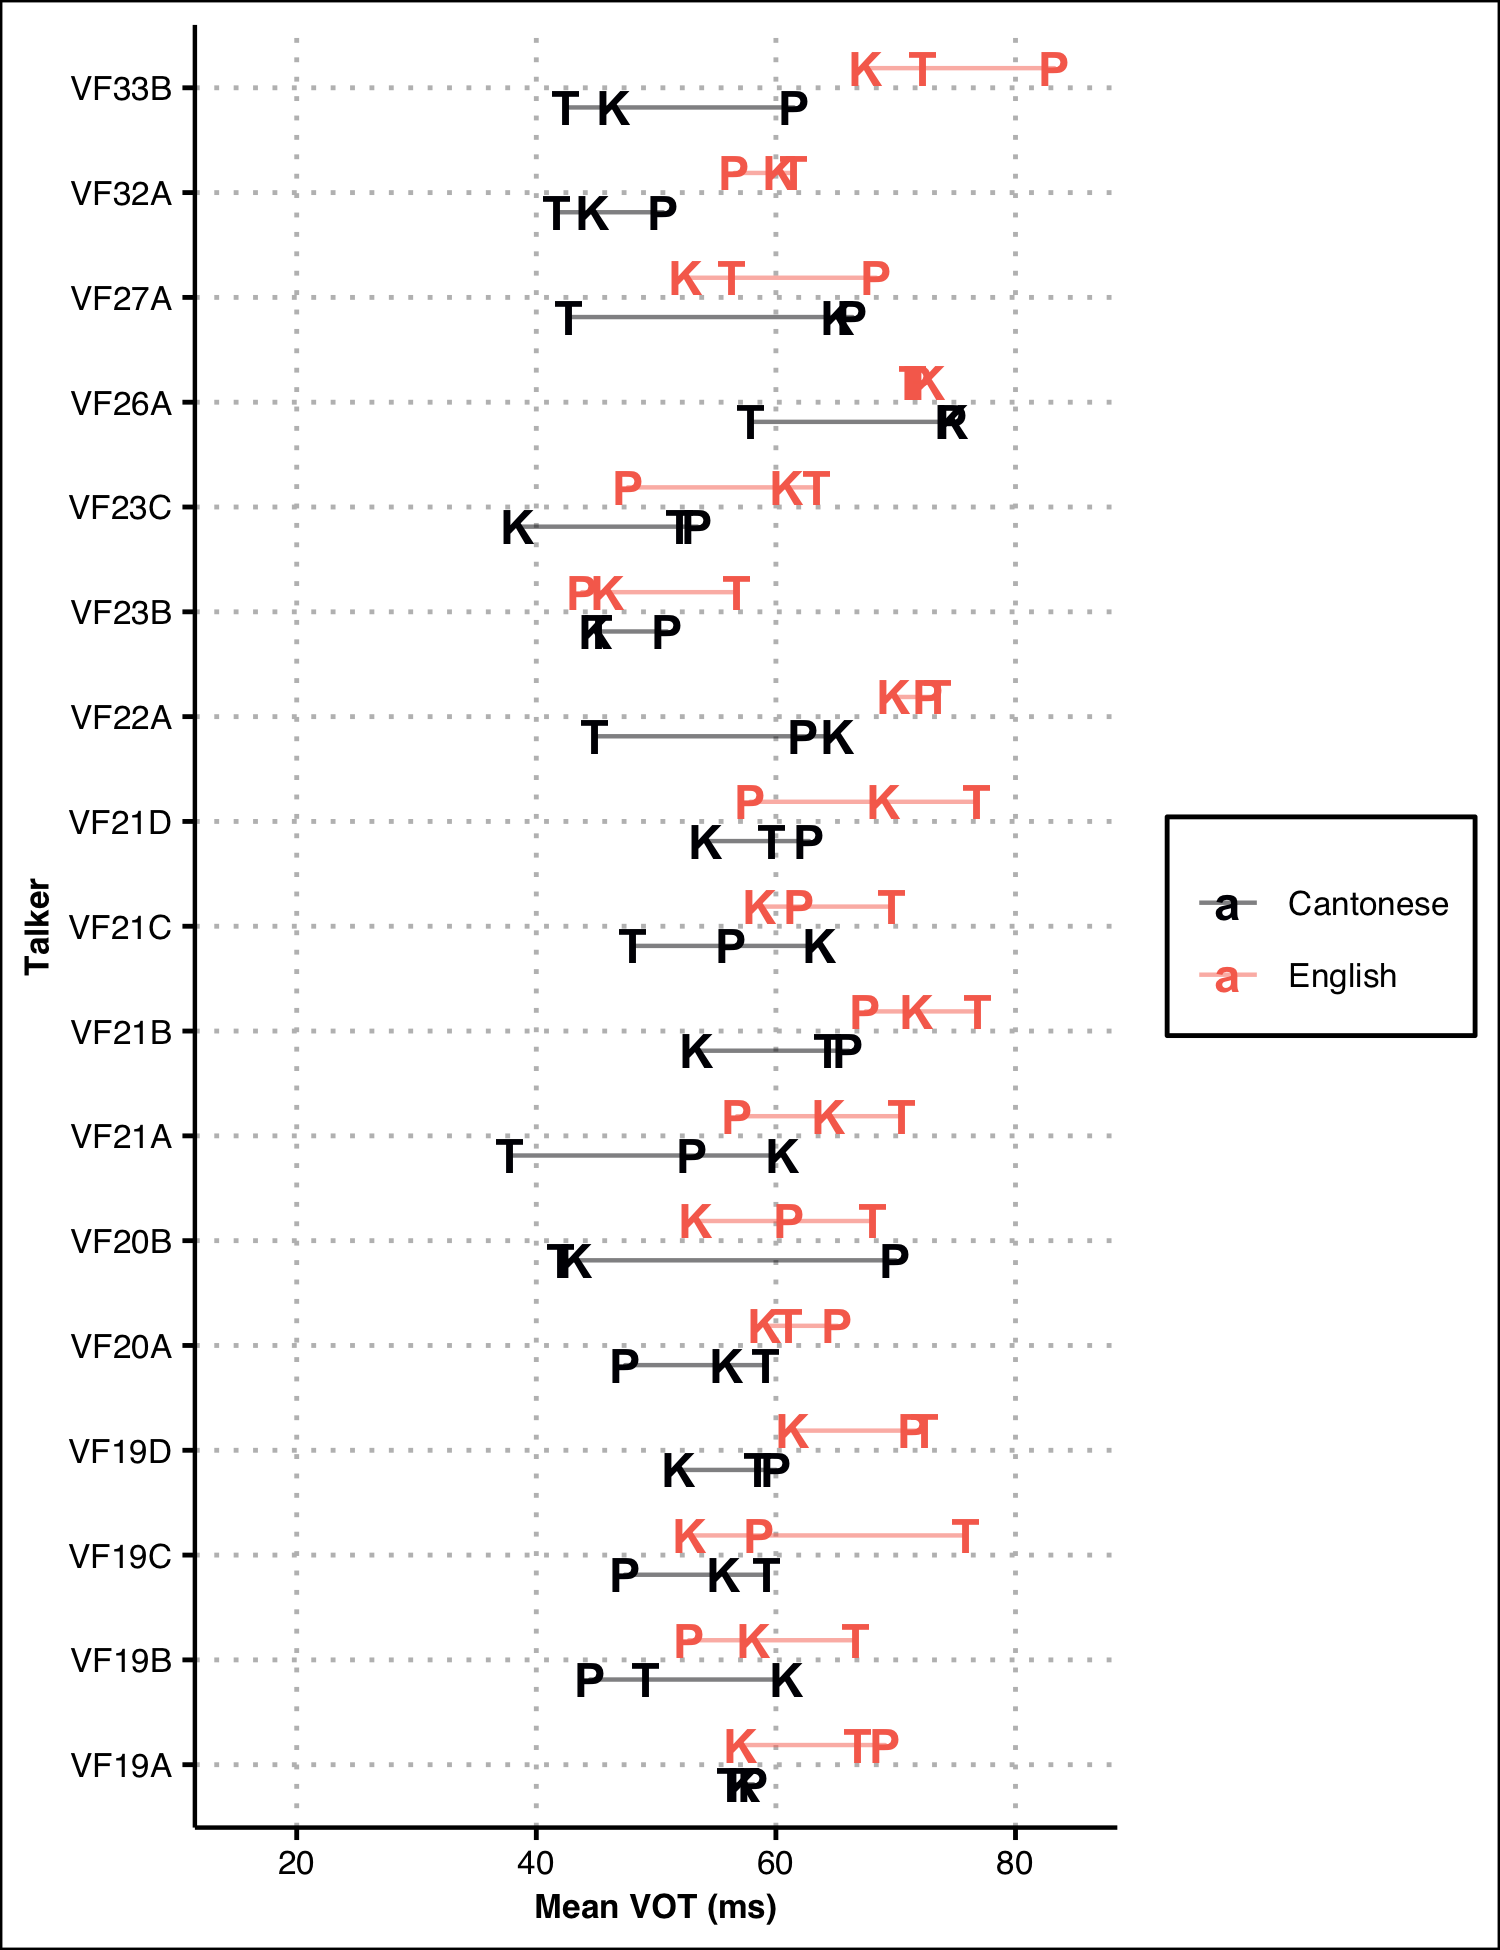
\includegraphics[width=0.9\linewidth]{figures/ch4_ordrel_vf_5in.png} 
  \caption{This figure depicts the ordinal relationships for the female talkers. Each panel depicts the mean VOT and standard error for VOT for each segment, with E(nglish) and C(antonese) in separate rows.}
  \label{ch4:fig:ordrelvf}
  \end{center}
\end{figure}

\begin{figure}[htbp]
  \begin{center}
  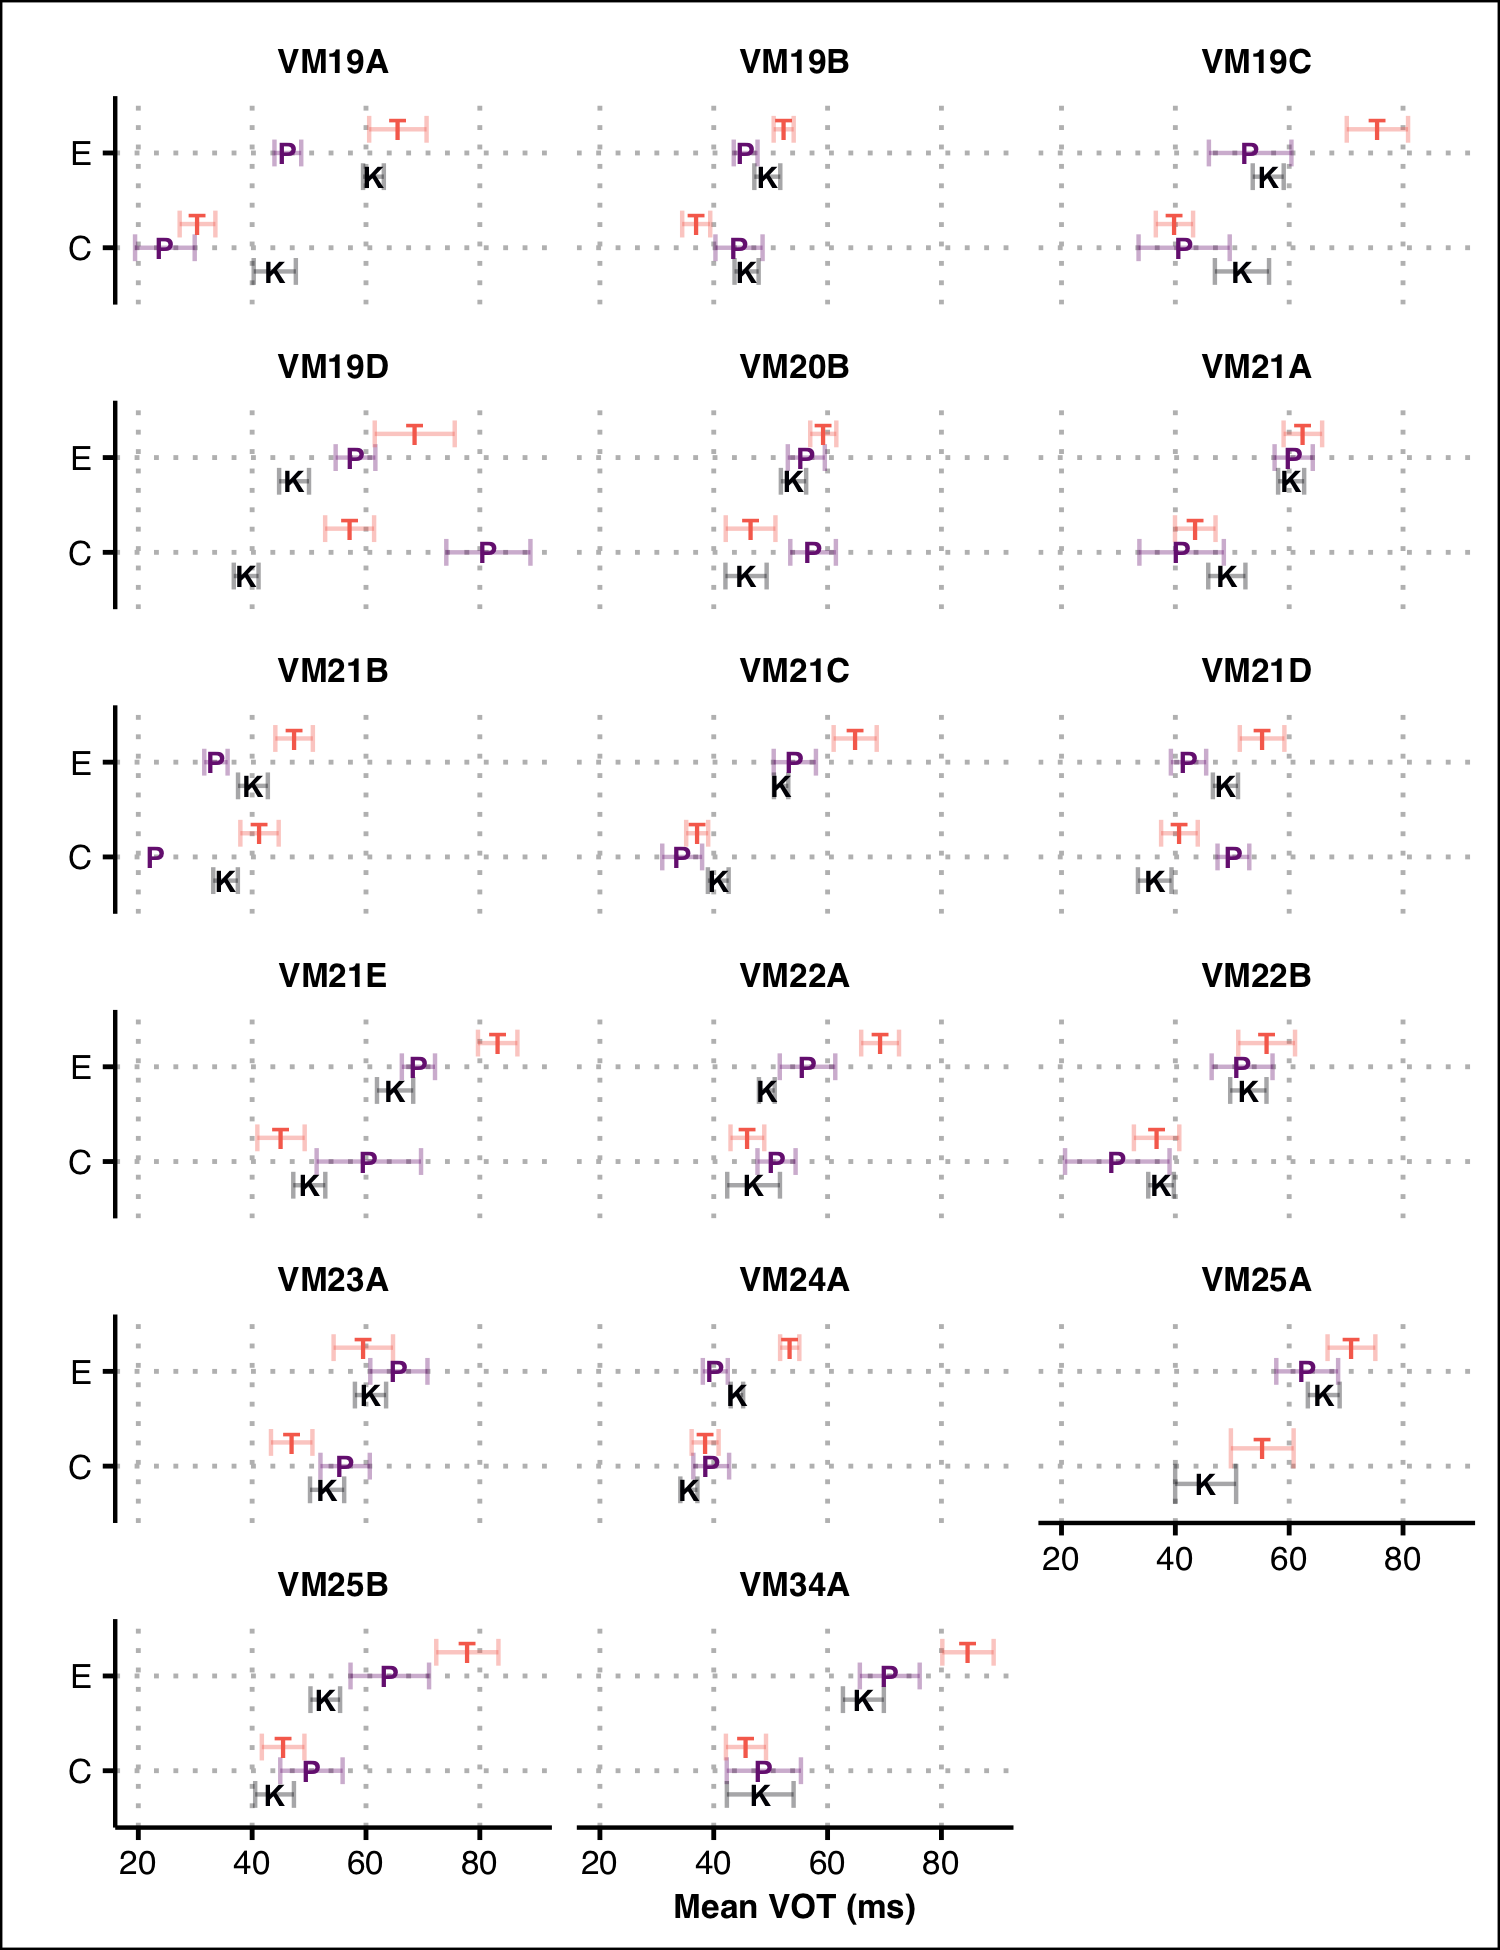
\includegraphics[width=0.9\linewidth]{figures/ch4_ordrel_vm_5in.png} 
  \caption{This figure depicts the ordinal relationships for the male talkers. Each panel depicts the mean VOT and standard error for VOT for each segment, with E(nglish) and C(antonese) in separate rows.}
  \label{ch4:fig:ordrelvm}
  \end{center}
\end{figure}


\subsection{Pairwise correlations}\label{ch4:sec:correlations}
% I personally don’t quite understand enough about your correlation analysis…a failing on my part, but maybe helped through extended discussion, is how sufficient using the residuals is for correcting for speech rate.
% it’s also unclear to me whether the talkers were paired with themselves within the correlations presented in Table 2 (i.e., are these analogous to the Chodroff and Wilson 2017 figures?)
% did you do any correction for significance with 15 correlations?
To examine the relationship between stops within and across languages, 15 pairwise Pearson's \textit{r} correlations were calculated across talker means. Each correlation compares talkers means for two different segments. The full pairwise correlations include three within English, three within Cantonese, and nine comparing English to Cantonese. These correlations are reported along with Holm-adjusted \textit{p}-values to account for multiple comparisons. This analysis uses the \textit{psych} \citep{revelle_2021_psych} package in R \citep{r_2021}. As in \citet{chodroff_2017_structure}, this correlation analysis aims to elucidate within-talker invariance and between-talker variability. While using means ignores information about within-category variability, prior work sets up strong, clear expectations about how the mean values for long-lag VOT pattern \citep{chodroff_2017_structure, cho_1999_vot}. 

Table \ref{ch4:tab:correlations} summarizes the output of all 15 correlations in text form. Figures \ref{ch4:fig:correlations1} and \ref{ch4:fig:correlations2} depict each of the 15 correlations in the fashion of \cite{chodroff_2017_structure}. While there is some evidence for both within- and across-language structured variation, the correlations reported here are considerably lower than prior work on English read speech. Similar within-language comparisons had $r>0.7$ \citep{chodroff_2017_structure, chodroff_2019_l2}. With the exception of the English /p/ $\sim$ /k/ ($r=0.70$, $p<0.001$), all of the correlations were either moderate ($0.5<r<0.7$; $p<0.01$) or not significant. Within-English correlations were the most consistent---all three had \textit{r} at or above 0.65 (p $<$ 0.001). Of the within-Cantonese correlations only /p/ $\sim$ /t/ was significant (\textit{r}$=$ 0.59; \textit{p}$=$0.003), though the correlation for /p/ $\sim$ /k/ was marginal (\textit{r}$=$ 0.44; \textit{p}$=$0.08). Two of three across-language correlations at the same place of articulation were significant, with moderate \textit{r} values (/p/ $\sim$ /p/: \textit{r}$=$0.62, \textit{p}$=$0.001; /k/ $\sim$ /k/: \textit{r}$=$0.57, \textit{p}$=$0.004). Of the across-language comparisons that do not share a place of articulation, only one was significant---Cantonese /k/ $\sim$ English /p/ (\textit{r}$=$0.58, \textit{p}$=$0.003).

\begin{figure}[htbp]
  \begin{center}
  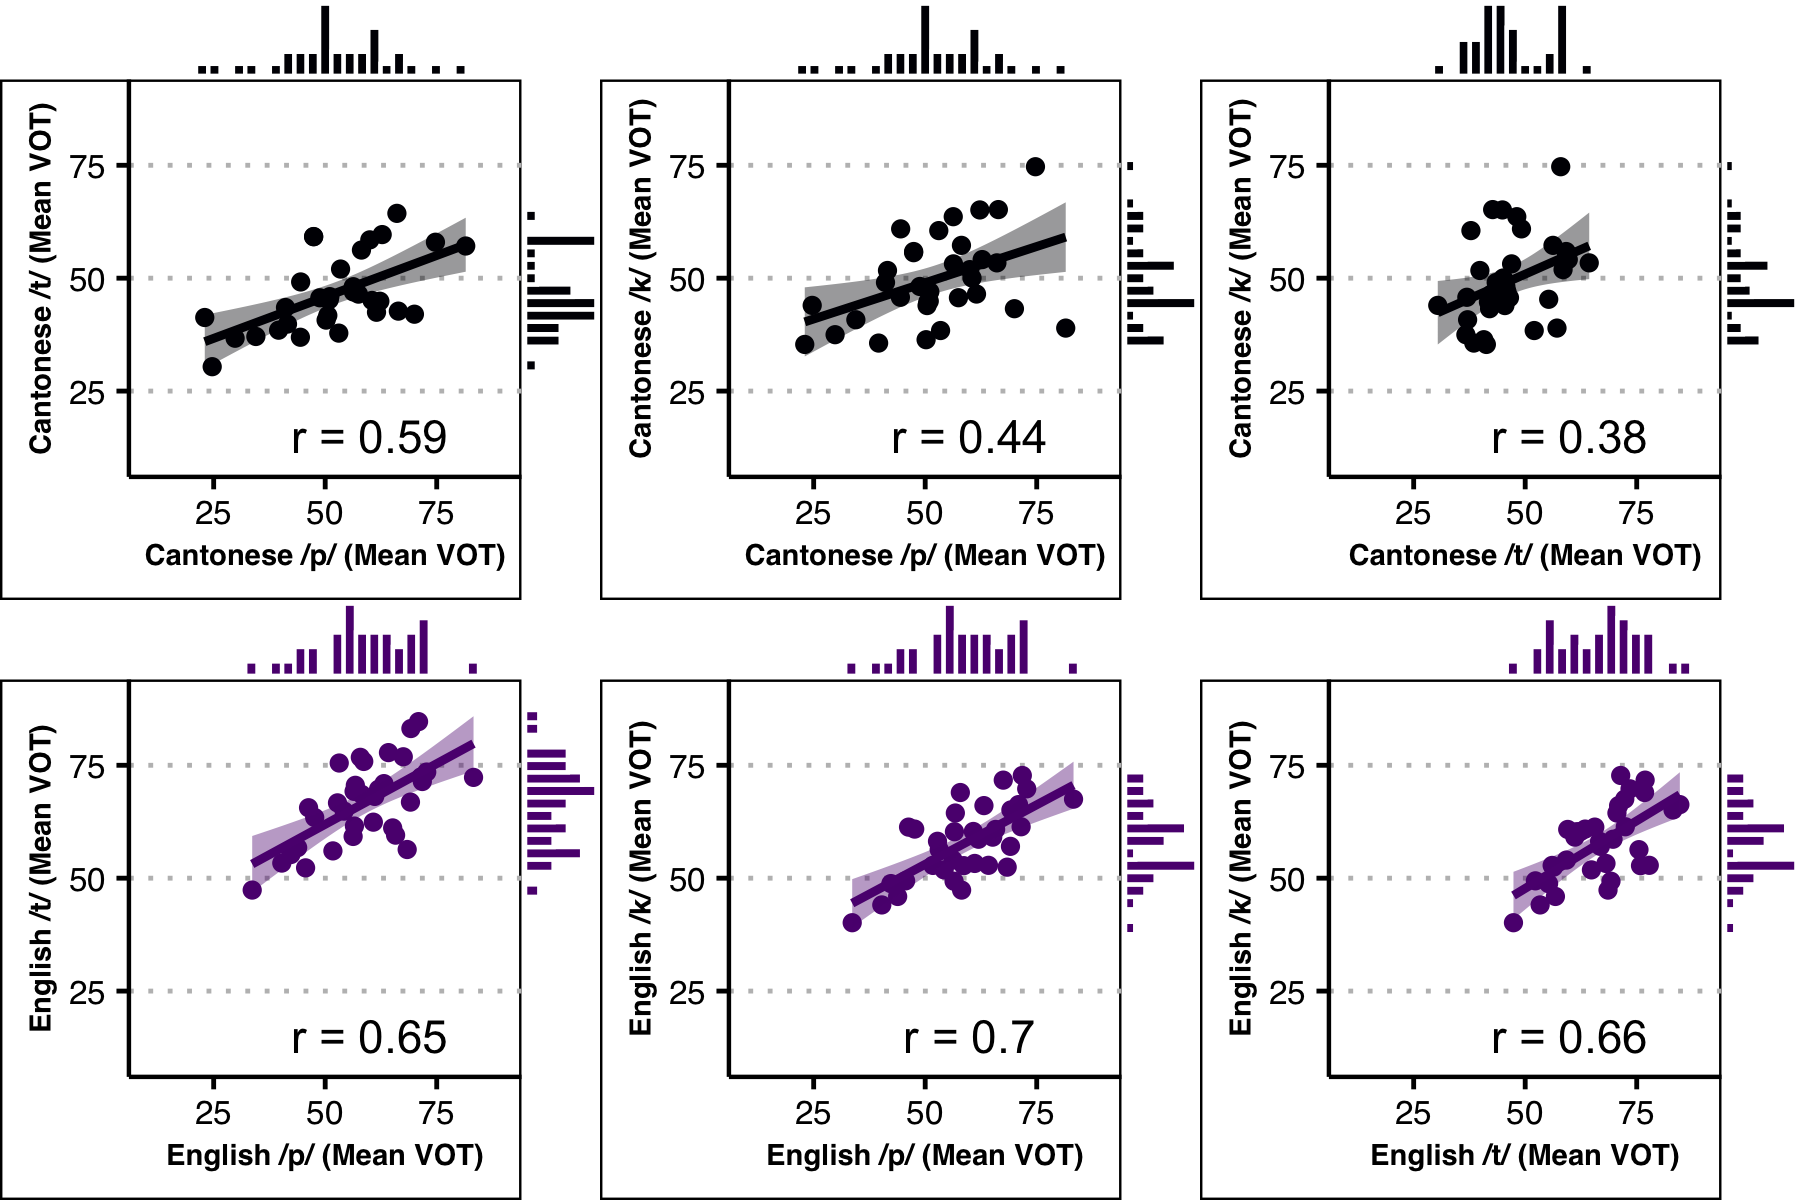
\includegraphics[width=0.9\linewidth]{figures/ch4_correlations1_5in.png} 
  \caption{Correlations!}
  \label{ch4:fig:correlations1}
  \end{center}
\end{figure}

\begin{figure}[htbp]
  \begin{center}
  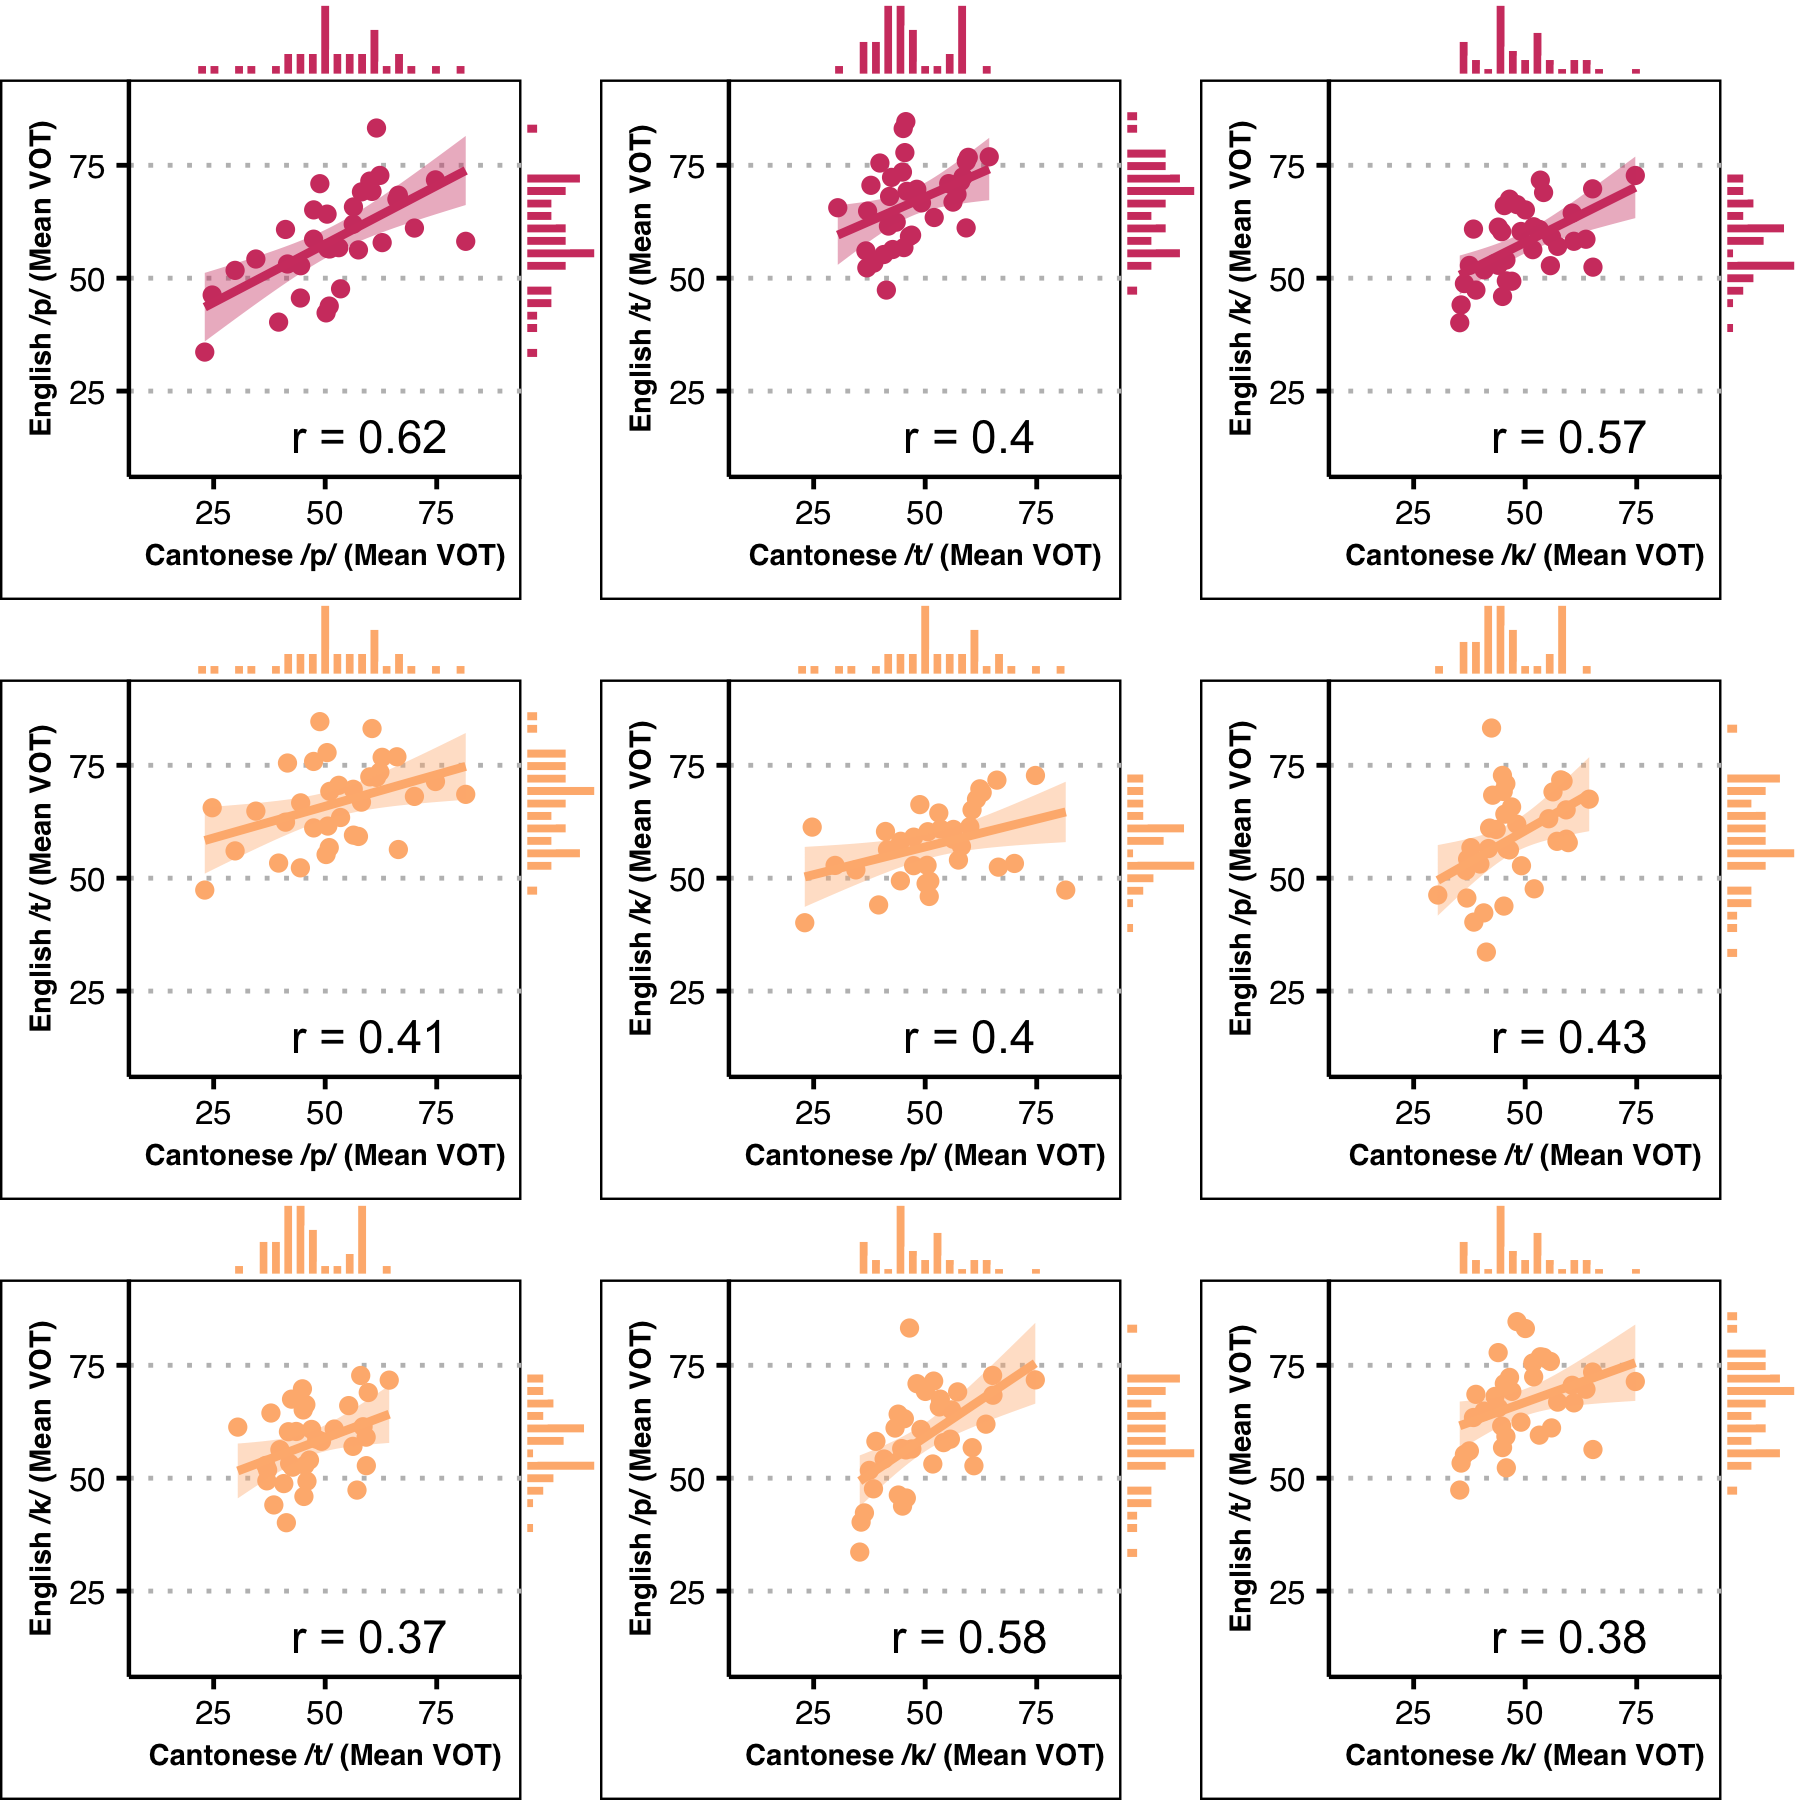
\includegraphics[width=0.9\linewidth]{figures/ch4_correlations2_5in.png} 
  \caption{Correlations!}
  \label{ch4:fig:correlations2}
  \end{center}
\end{figure}

\begin{table}[htbp]
  \caption{All 15 correlations based on raw mean VOT---and separately, VOT residuals after accounting for speaking rate---for each talker, language, and segment. Each row indicates the comparison, Pearson's \textit{r}, and the Holm-adjusted \textit{p}-value given 15 comparisons.}
    \label{ch4:tab:correlations}
    \centering 
    \footnotesize
    \begin{tabular}{ll|ll|ll}
      \toprule
      &   & \multicolumn{2}{l|}{\textbf{Raw}} & \multicolumn{2}{l}{\textbf{Residualized}} \\
      \textbf{Type}     & \textbf{Comparison} & \textit{r}        & \textit{p}       & \textit{r}            & \textit{p}            \\
    \midrule
    Within-Cantonese  & Cantonese /p/ $\sim$ Cantonese /t/    & 0.59    & 0.003       & 0.59   & 0.003    \\
    Within-Cantonese  & Cantonese /p/ $\sim$ Cantonese /k/    & 0.44    & 0.08        & 0.55   & 0.01     \\
    Within-Cantonese  & Cantonese /t/ $\sim$ Cantonese /k/    & 0.38    & 0.11        & 0.34   & 0.21     \\
    \midrule
    Within-English    & English /p/   $\sim$  English /t/     & 0.65    & $<$0.001    & 0.63   & 0.001    \\
    Within-English    & English /p/   $\sim$  English /k/     & 0.70    & $<$0.001    & 0.70   & $<$0.001 \\
    Within-English    & English /t/   $\sim$  English /k/     & 0.66    & $<$0.001    & 0.60   & 0.002    \\
    \midrule
    Across-language   & Cantonese /p/  $\sim$ English /p/     & 0.62    & 0.001       & 0.57   & 0.01    \\
    Across-language   & Cantonese /t/  $\sim$ English /t/     & 0.40    & 0.11        & 0.35   & 0.21    \\
    Across-language   & Cantonese /k/  $\sim$ English /k/     & 0.57    & 0.004       & 0.54   & 0.01    \\
    \midrule
    Across-language   & Cantonese /p/  $\sim$ English /t/     & 0.41    & 0.11        & 0.29   & 0.31    \\
    Across-language   & Cantonese /p/  $\sim$ English /k/     & 0.40    & 0.11        & 0.29   & 0.31    \\
    Across-language   & Cantonese /t/  $\sim$ English /p/     & 0.43    & 0.08        & 0.37   & 0.20    \\
    Across-language   & Cantonese /t/  $\sim$ English /k/     & 0.37    & 0.11        & 0.27   & 0.31    \\
    Across-language   & Cantonese /k/  $\sim$ English /p/     & 0.58    & 0.003       & 0.59   & 0.003   \\
    Across-language   & Cantonese /k/  $\sim$ English /t/     & 0.38    & 0.11        & 0.37   & 0.20    \\
    \bottomrule
    \end{tabular}
\end{table}

\citet{chodroff_2017_structure} also repeat the correlation analysis in a way the coarsely accounts for speaking rate. This consideration is important, as the local speaking rate is known to influence long-lag VOT in spontaneous speech \citep{stuartsmith_2015_private} and because prior work demonstrates both talker and language effects on speech rate \citep{bradlow_2017_rate}. In comparing the two versions of the correlation analysis, \citeauthor{chodroff_2017_structure} found that ``the magnitudes of the correlations among voiceless stops did not deviate from the original magnitudes, demonstrating that differences among talkers in the realization of these sounds cannot be reduced to talker-specific speaking rates'' \citeyearpar[][p. 34]{chodroff_2017_structure}. 

I conducted a similar analysis here, using means calculated over \textit{residual} VOT values from a simple linear regression in which VOT was predicted by average phone duration within the word. Average phone duration is a proxy for speech rate. It was calculated as the difference between the word's AutoVOT-estimated onset and force-aligned offset, divided by the number of segments in the canonical form of the word. The results---Pearson's \textit{r} and Holm-adjusted \textit{p} values---are reported in the rightmost columns of Table \ref{ch4:tab:correlations}. Qualitatively, the results mostly mirror the correlations based on raw VOT, though there are some differences in significance and magnitude. This difference can likely be attributed to the generally weak correlations found. 

While these relationships indicate some degree of articulatory reuse, the overall picture is far from compelling, particularly when considered alongside the results of the analysis of the ordinal relationships in Section \ref{ch4:sec:ordrel}. Compared to prior work, these correlations are less consistent and generally weaker.

The next steps in \citeauthor{chodroff_2017_structure}'s \citeyearpar{chodroff_2017_structure} methods focus on validating the strength of the correlations. Their approach includes estimating confidence intervals for the correlations using a bootstrap procedure \citep{chodroff_2017_structure}. In a later paper, they simulate what would emerge from a purely ordinal relationship between stops and demonstrate that the observed correlations are much stronger—ultimately arguing for a uniformity constraint on phonetic variation \citep{chodroff_2019_covariation}. Given that the correlations found in this chapter are drastically lower and largely do not adhere to the expected ordinal relationships, the remainder of this analysis takes a different approach.

\subsection{Linear mixed effect model}\label{ch4:sec:lmem}

The analysis in the section leverages a Bayesian multilevel linear model to elucidate the sources of variation within and across talkers. As Bayesian modeling emphasizes the estimation of effect magnitudes, the model can be used to assess how talker's sound categories compare to one another while simultaneously accounting for factors known to influence long-lag VOT. This modeling approach is more in line with the generative modeling approach advocated for by \citet{haines_2020_theoretically}---in a way that the correlation and ordinal relationships analyses in the preceding sections are not. This section proceeds as follows. Section \ref{ch4:sec:bayesianinference} describes Bayesian modeling and inference in broad terms and points the reader towards sources for further reading. Section \ref{ch4:sec:model} motivates and describes the structure of the model used in this chapter. Lastly, Section \ref{ch4:sec:results} reports the results of the model. All code used in this analysis is available at \hl{a GitHub repository that will be made public later on}.

\subsubsection{Bayesian inference}\label{ch4:sec:bayesianinference}
The corpus sample was analyzed with a Bayesian multilevel linear model using the brms package in R \citep{burkner_2017_brms,r_2021}. The brms package provides a simple, formula-based interface to Stan---a widely used probabilistic programming language for estimating Bayesian statistical models \citep{stan_2021}. Bayesian models are desirable in the case of modeling multilingual VOT for both practical and theoretical reasons. Practically, they are not subject to the convergence problems that plague complex frequentist models. Theoretically, they allow for graded statements regarding the strength of evidence for all parameters, both population level (i.e., fixed effects) and group level (i.e., random effects) parameters. While there are many other benefits, readers are referred to \citeauthor{vasishth_2018_bayesian}'s \citeyearpar{vasishth_2018_bayesian} recent in-depth tutorial paper on Bayesian modeling in the phonetic sciences for further argumentation. 

Inference in Bayesian models is based on the posterior distributions of parameters in the model, which reflect the range and probability of credible values for parameters. The posterior combines information from prior knowledge and the likelihood of observing the data given the specified model. While some Bayesian models use detailed and specific prior knowledge, it is perhaps more common to use weakly informative, regularizing priors \citep{gelman_2017_prior}, which constrain the parameter space to possible values and down weight extreme or unlikely values. The model described in the next section uses regularizing priors. 

In line with how Bayesian models emphasize parameter estimation in a probabilistic framework, it is also possible to compare parameters. \citet{gelman_2012_multiple} argues that because of the rich probabilistic information in each parameter's posterior distribution, making multiple comparisons within the model is not problematic, as it is in the case of frequentist statistics. Further, while parameter estimation remains the focus, there are decision criteria that facilitate determining whether the difference between two parameters is important or not. One such technique is to use \citeauthor{kruschke_2011_rope}'s \citeyearpar{kruschke_2011_rope} ROPE+HDI method. The ROPE is a ``region of practical equivalence'' surrounding the null value. The HDI is the highest density interval typically used to describe Bayesian posterior distributions. \citeauthor{kruschke_2011_rope}'s \citeyearpar{kruschke_2011_rope} decision criterion is simple: if the HDI falls entirely within the ROPE, then the null value can be accepted; if the HDI falls entirely outside the ROPE, then it can be rejected; if there is overlap, then a decision should be withheld. In the case of standardized data, \citet{kruschke_2011_rope} recommends the convention of setting a ROPE to be [$-$0.1, 0.1]---half the size of a small Cohen's \textit{d} effect. While Bayesians tend to shy away from using decision criteria, it nonetheless provides a useful scaffolding for interpreting the magnitudes of standardized effects, when presented alongside the full posterior distributions. 

\subsubsection{Modeling multilingual VOT}\label{ch4:sec:model}

VOT was modeled using a multilevel generallized linear with a log-normal repsonse variable distribution. Using a log-normal response distribution is appropriate in the case of VOT, as possible long-lag VOT values are positive. Given this lower bound, it follows that the distribution will have a right tail. This is refelcted in prior work log-transforming VOT prior to linear modeling \citep[e.g.,][]{stuartsmith_2015_private}. It also represents one of the key tenets of building theoretically informed models, as advocated for by \citet{haines_2020_theoretically}. The model used in this section was the following:

\begin{equation}
  \begin{aligned}\label{ch4:num:formula}
    \text{VOT } \sim \text{ 1 } + \text{ Place } \times \text{ Language } + \text{ Average Phone Duration } + \text{ Pause } + \text{ } \\
    (\text{1 } + \text{ Place } \times \text{ Language }|\text{ Talker}) + (\text{1 }| \text{ Word}) \text{\medskip}
  \end{aligned}
\end{equation}

So while the formula in \ref{ch4:num:formula} does not represent the maximal model \citep{barr_2013_maximal}, it instead follows guidelines for parsimonious model building \citep{bates_2018_parsimonious}, in which the parameters of direct interest are included as random slopes, and the controlling parameters are not. 

% The interpretation of the linear ME model needs to be fleshed out and related more clearly to your original research question(s)
% Frame this section as being motivated by the lack of strong uniformity, and by Chodroff's analysis of the random effects structure
% To better account for variation due to known factors such as speech rate and the presence of a preceding pause, a linear mixed-effects model was fit with the \textit{lme4} package \citep{bates_2015_lme4} in R \citep{r_2021}. The model's aims were two-fold: estimating the effect of language by segment and elucidating the sources of variation in the random effects structure. Analyzing the data in this way mitigates the issues with conducting statistical tests on talker means, which ignores much of the variation in the data \citep{haines_2020_theoretically}. 

One of the main benefits of multilevel modeling is partial pooling, where information for different levels of a variable is shared across those levels. \citeauthor{mcelreath_2020_sr} argues that ``any batch of parameters with exchangeable index values can and probably should be pooled [where exchangeable] just means the index values have no true ordering'' \citeyearpar[][p. 435]{mcelreath_2020_sr}. Pooling can be done for both intercepts and slopes, much in the way that frequentist models allow for slopes and intercepts to vary in the random effects structure. As apparent in the formula in \ref{ch4:num:formula}, this model includes partial pooling for all of the parameters of interest. Details about how the parameters were specified are as follows.  

\begin{description}
  \item[VOT] was the dependent variable---it was scaled (i.e., divided by the standard deviation), in order to facilite the specification of priors and a ROPE. VOT was \textit{centered}, however, as the log-normal distribution requires positive values in the response variable distribution.
  % \item[Phone] encodes both place of articulation and language, such that there are six levels---one for each phone in each language. Phone uses index variable coding, as advocated for by \citet{mcelreath_2020_sr}. This means that the model estimates a separate intercept for each of the phones, but not an overall intercept. Ultimately, this facilitates the comparisons of interest.
  \item[Place] encodes place of articulation for the stops and has three levels. Following \citet{chodroff_2017_structure}, Place was weighted effect coded in order to account for unequal sample sizes across the three levels and to faciliate the interpretation of the simple effects in light of the interaction term \citep{brehm_2021_contrasts}. Coding was implemented using the \textit{wec} package \citep{nieuwenhuis_2017_weighted}, and results in reporting Place effects for T (weights: /p/ $=-1.92$, /t/ $=1$) and K (weights: /p/ $=-3.44$, /t/ $=10$, /k/ $=1$).
  \item[Language] is a binary variable that encodes whether the VOT measurement comes from an English or Cantonese word. As with Place, Language was also weighted effect coded (Cantonese $=-1.61$, English $=1$).
  \item[Average Phone Duration] represents the average duration of phones within the word. It was calculated as the difference between the word's AutoVOT-estimated onset and the force-aligned word offset, divided by the number of segments in the canonical form of the word. As noted earlier, average phone duration serves as a proxy for local speaking rate. A word-internal measure is desirable, as many tokens were preceded by a pause and thus lack the preceding context from which to calculate it. Average phone duration was standardized---that is, both centered and scaled. 
  \item[(Preceding) Pause] indicates whether or not the token occurred after a pause or not. Pauses were defined as X. The presence of a preceding pause was also implemented with weighted effect coding (False $=-0.33$, True $=1$).
  \item[Word] indicates the word that the VOT measurement comes from. 
\end{description}

The interaction for Language $\times$ Place was included in the model---it directly addresses the research question relating to whether or not bilinguals maintain a difference across languages for these sounds. Additionally, the model includes partial pooling (i.e., random intercepts) for Word and Talker, as well as for the Language, Place, and Language $\times$ Place terms (i.e., random slopes). 

\subsubsection{Results}\label{ch4:sec:results}




% Add full table of LME results and some data viz

% At an $\alpha=0.01$ threshold, the model returned a significant intercept ($\beta=0.18$, $SE=0.49$, $p<0.001$), significant main effects for Average Phone Duration ($\beta=0.32$, $SE=0.01$, $p<0.001$) and Preceding Pause (True; $\beta=0.12$, $SE=0.02$, $p<0.001$), as well as significant simple effect for Language (English; $\beta=0.15$, $SE=0.03$, $p<0.001$), indicating that VOT was longer at slower speech rates, after pauses, and in English, compared to the weighted mean. Neither Place nor its interaction with Language was significant. As one of the linear mixed-effects model goals was to assess the effect of Language across places of articulation, pairwise post-hoc comparisons were computed for Language $\times$ Place using the \textit{emmeans} package \citep{lenth_2021_emmeans}, with a confidence level of 0.95, and the Kenward-Roger degrees-of-freedom method. The contrast between languages was significant for /t/ ($\beta=-0.38$, $SE=0.09$, $p<0.001$) and /k/ ($\beta=-0.53$, $SE=0.10$, $p<0.001$), but not for /p/ ($\beta=-0.09$, $SE=0.11$, $p=0.39$): VOT is consistently longer in English for /t/ and /k/.

% The second goal of the mixed-effects analysis was to gain insight into the sources of variation through the random effects structure. Of the random effects, the intercepts for Word ($SD=0.20$) and Talker ($SD=0.06$) accounted for the most variation, followed by the by-Talker slope standard deviations for Language ($SD=0.005$), Place T ($SD=0.01$), Place T $\times$ Language ($SD=0.005$), Place K ($SD=0.004$) and Place K $\times$ Language ($SD=0.002$). Talkers and words differ substantially in mean VOT, while the slopes for Place and Language effects appear more consistent across talkers.





\section{Discussion}
% ADD:
% - Limitation of whether the difference between languages is a clear diff, or motivated by timing differences, e.g. Bradlow's speech rate paper as a potential avenue to disambiguate this -> both language and talker-indexical info there

This paper reports a study of long-lag stops in Cantonese-English bilingual speech from the SpiCE corpus described in Chapter \ref{ch:Corpus}. It uses the uniformity framework to assess VOT similarity within and across languages. In broad strokes, the evidence for uniformity both within and across languages was limited. The correlation analysis provides evidence for within-language uniformity and some across-language structure. The magnitudes were largely weak and moderate. These results are corroborated by the random effects structure of the linear mixed-effects model, as more of the variation is attributable to Talker intercepts than to the Language and Place slope effects. In this sense, while there is some degree of structure in VOT variation, it seems weaker than the relationships described in prior work, where strong and clear within-language patterns were observed \citep{chodroff_2017_structure, chodroff_2019_l2}.

The far more interesting outcomes here relate to unexpected results. The ordinal relationships should be interpreted with a grain of salt, as there are several potential explanations not immediately relevant to the research question. For example, means were based on fewer tokens than in prior work (especially for /p/), which may render those proportions less reliable; and, the speech in SpiCE differs in style (conversational vs. read). This outcome is perhaps not surprising, as \citet{chodroff_2017_structure} reported magnitude differences between isolated citation form and connected read speech. Lastly, the error often overlaps in Figure XX, potentially making the ordinal relationships less reliable or meaningful. Another unexpected outcome is that English VOT seems to be consistently longer than in Cantonese---the opposite of what prior work suggested \citep{clumeck_1981_cantonese, lisker_1964_vot}. No explanation is offered here other than to reiterate the casual speech style under examination. Additionally, lab and corpus results often differ \citep{gahl_2012_reduce,chodroff_2017_structure}, as do corpus studies of monolingual and bilingual speech \cite{johnson_2019_probabilistic}. 

While the results here do not necessarily provide evidence for a bilingual crosslinguistic uniformity constraint, they offer insight into what makes bilingual speech unique and provide an empirical description of bilingual long-lag stops. In terms of describing the relationship between the long-lag stops in each language, talkers maintain a crosslinguistic contrast despite stops' proximity---for many talkers---in the long-lag space. The contrast is a strong candidate for a composite category in SLM-r \citep{flege_2021_slmr} and merits further investigation.

% Flesh out this paragraph a bit more, but save something for the general discussion -->
A lack of strong crosslinguistic uniformity has implications for speech perception. Tracking a uniformity-like pattern has been proposed as a mechanism for rapidly adapting to speech across languages \citep{reinisch_2013_retune} and in multilingual talker identification \cite{orena_2019_identifying}. If the results of this study stand, then such a perceptual strategy may have limited use in real communicative contexts, whether or not listeners use it in a lab setting. Overall, this study highlights the need to study spontaneous speech and offers a first pass at leveraging the methods of the uniformity framework to better understand crosslinguistic similarity.

\endinput % -------------------------------------------------------- %

% THE GRAVEYARD OF WORDS


% Define representation, phonetic categories, and exemplar-y model, what it means for categories to be linked, i.e., the composite category of SLM-r

% A consequence of bilingualism is that individuals must navigate overlapping segment inventories. This paper is concerned with what languages share, if anything, in the mental representation of speech sound categories. As representation means different things across linguistic disciplines, defining and situating the term is first necessary. The approach in this chapter largely falls out of the revised Speech Learning Model \citep[SLM-r;][]{flege_2021_slmr} and its exemplar-flavored take on what phonetic categories look like in linguistic systems with more than one language. 

% SLM-r is a widely used and respected model used in second language acquisition and multilingualism research. Unlike some other models in the same space, SLM-r grapples with both perception and production. SLM-r assumes that speech sound categories from different languages exist in a shared phonetic space and are subject to constraints from the perceptual and productive systems. Effectively, don't get too close to each other in perception, and don't get too complicated in production \citep{guion_2003_systems, lindblom_1988_universals, flege_1995_slm}. These constraints lead SLM-r to posit that proximity leads to instability, even if what counts as close remains unclear. Considering how bilinguals are fully capable of maintaining subtle distinctions for similar sound categories across languages \citep[e.g.,][]{sundara_2006_production}, this is not a trivial point to make. 

% So, what does representation look like in this system? SLM-r outlines a few potential outcomes for sound categories in a shared system—they can assimilate or dissimilate. A relatively simple take on this is that assimilation equals shared mental representation, while dissimilation equals separate. The picture is complicated, however, by the idea of imperfect assimilation and what \citeauthor{flege_2021_slmr} term \textit{composite categories}. In the SLM-r, if sounds from two languages are phonetically too close to each other, they will remain linked in a composite category "defined by the statistical regularities present in the combined distributions of the perceptually linked...sounds." \citep[][p. 41]{flege_2021_slmr}. This scenario might be characterized as an imperfectly shared representation, where certain dimensions are kept apart, and others overlap. This particular characterization is salient in a recent meta-analysis of crosslinguistic influence for Spanish and English initial stop consonants. In this study, \citet{casillas_2021_interlingual} found that early bilinguals did not produce ``compromise'' stop categories. That is, early Spanish-English bilinguals did not produce voice onset time that was somehow intermediate to canonical productions by monolinguals of either language. This finding echoes arguments made by \citet{bullock_2009_sociophonetics} on the sophistication and control that bilingual exert over their possible forms. There is no compromise but rather a wide range of forms that bilinguals can deploy according to context.

% % Need to fix a lot in here because Casillas paper really goes against the idea of composite or "compromise" categories

% This idea of composite categories is similar to other concepts in multilingualism literature, namely that of linked categories. While the idea is pervasive, it is somewhat vaguely defined. In a handbook chapter on bilingual phonetics and phonology, \citet{simonet_2016_bilingualism} describes ``links or connections of one sort or another between the phonetic categories'' (p. 10). \citeauthor{simonet_2016_bilingualism} then notes that ``these connections...are transiently strengthened in contexts that induce the activation of both languages and inhibited in contexts that favor the use of only one of the languages'' \citeyearpar[][p. 10]{simonet_2016_bilingualism}. Presumably, sound categories could be linked whether they surface in dissimilated or composite (assimilated) forms. The idea behind composite categories is more fully fleshed out and theoretically useful than mere links in grappling with how representation works in the bilingual mind. 

% Most prior work in crosslinguistic influence has focused on sounds that are phonologically similar yet phonetically distinct. A common example of this arises from languages that differ in their initial stop voicing contrasts. North American English contrasts long- and short-lag stops in initial position. Conversely, Spanish (among many languages) contrasts short-lag and prevoiced initial stops. As will become apparent later in the introduction, there is strong evidence for a crosslinguistic link between English long-lag and Spanish short-lag stops, despite the clear difference in voice onset time. The relative position of these sounds within each language can account for why they are linked together; in each case, the linked sound occupies the position closest to long-lag, on a spectrum ranging from long-lag to short-lag to prevoiced. The primacy of ``relative phonetics'' was put forth in \citeauthor{chang_2015_similarity}'s \citeyearpar{chang_2015_similarity} chapter on similarity in bilingual phonetics and phonology. \citeauthor{chang_2015_similarity} argues that crosslinguistic influence at the segmental level tends to occur between sounds that share ``(1) similar positions in the respective phonemic inventories (when considering the contrastive feature oppositions---or, more broadly, the `relative phonetics'---of the sounds in relation to other sounds in the inventory), and (2) similar distributional facts'' \citeyearpar[][p. 201]{chang_2015_similarity}. This approach to similarity emphasizes a general role for abstraction but does not necessarily invite a formal phonological analysis. In a similar vein, \citeauthor{flege_2021_slmr} argue that similarity ``must be assessed perceptually rather than acoustically because acoustic measures sometimes diverge from what listeners perceive'' \citeyearpar[][p. 33]{flege_2021_slmr}. At this point, ``relative phonetic'' and perceptual similarity seem to be a prerequisite for considering a link between two sound categories and can be used to account for when and where crosslinguistic influence occurs. It does not outline what happens after sounds are ostensibly linked to one another nor opine on the nature of representation for the sound categories in question. 

% \citeauthor{flege_2021_slmr} make a clear appeal to phonetic similarity for assessing assimilation. This appeal is evident in how it steps back from making phonological arguments in general and in its exemplar-flavored account. The SLM-r posits that sound categories ``are defined by the statistical properties of input distributions'' \citeyearpar[][p. 40]{flege_2021_slmr}. In the case of assimilation, there is a single distribution for both languages---a shared representation. Composite categories are considered a special type of assimilation in the SLM-r, though given the results of \citeauthor{casillas_2021_interlingual}'s \citeyear{casillas_2021_interlingual} meta-analysis, they may not be an appropriate characterization of early bilinguals' systems. In the case of dissimilation, the sound categories move apart and comprise separate distributions---separate representations. While \citeauthor{flege_2021_slmr} argue that crosslinguistic influence provides a diagnostic to test for the presence or absence of dissimilation, but also state that ``A method did not exist in 1995 for determining when a new L2 phonetic category had been formed and, alas, the same holds true today'' \citeyearpar[][p. 41]{flege_2021_slmr}. It can be surmised from this that crosslinguistic influence is not a perfect diagnostic. 

% % the flow is off in this part

% In any case, the focus on distributions of experienced exemplars fits in well with the psycholinguistics literature that argues for the primacy of position-specific allophones \citep{mitterer_2018_allophones}, against the use of phonological features in accounting for speech behavior \citep{llompart_2018_acoustic}, and against equating theoretical categories with mental categories more broadly \citep{samuel_2020_resist}.

% The theoretical framework adopted here leans much harder into the phonetics side of the equation and takes exemplar-style sound categories for position-specific allophones as the level of abstraction. The specific categories considered in this chapter are likely subject to some form of assimilation. One of the questions taken up in this chapter is whether this assimilation is complete or takes the form of a composite category. In all cases, crosslinguistic influence---phonetic similarity or dissimiarily---for linked sounds is measured by comparing distributions of measurements, typically in the context of null hypothesis significance testing. The following paragraphs provide a review of the literature on crosslinguistic influence for stop consonants. 


% %Phonetic similarity is typically assessed by distilling either the entire signal () or a subset of relevant acoustic dimensions () and measuring the distance between relevant categories (e.g., Euclidean distance). Applying phonetic versions of similarity to bilingualism is straightforward, though it assumes that the measures used are appropriate in both languages. On the other hand, phonological similarity is typically assessed through distributional () or feature-based mechanisms (). Translating these phonological metrics to a bilingual system, however, is complicated. It requires making a multitude of assumptions about the nature of each language's inventory and ensuring some form of shared currency (i.e., a feature set). 

% % Define phonological similarity, and phonetic similarity, and what it means to be phonologically similar, but arise from a different part of the mental space, again i think exemplars and composite categories are the way to go here


% \hl{intro drafted up to here}

% More in depth review of CLI work -->
% One example is the comparison between initial voiceless stops in English (long-lag) and Spanish (short-lag). Despite the substantial phonetic differences, these sounds are clearly linked in the bilingual mind \citep{fricke_2016_phonetic, antoniou_2010_context, goldrick_2014_switching, sundara_2006_production}. 

% The following studies focus on telling initial stops apart when the stops under consideration are short-lag and long-lag stops, respectively. In most cases, the difference in voice onset time arises because the languages considered are English and a language with a different initial voicing contrast, as with the example given earlier in this chapter. 

% \hl{summary of lab CLI here} \citep{fricke_2016_phonetic, antoniou_2010_context, goldrick_2014_switching, sundara_2006_production}. % add more!

% These studies demonstrate phonetic convergence---or assimilation---in two ways. First, VOT is shorter for English initial stops produced by bilinguals when compared to monolingual control groups. This result is attributed to the influence on English long-lag stops from the short-lag category in the other language. Second, bilinguals appear more likely to produce lead voicing in initial English voiced stops compared to English monolinguals \citep{sundara_2006_production}. In both cases, evidence of crosslinguistic influence arises from comparing bilinguals to monolinguals. Corpus research demonstrates that Spanish-English bilinguals produce shorter, more Spanish-like VOT in the lead up to an English-to-Spanish code switch \citep{fricke_2016_phonetic, bullock_2009_sociophonetics}. 

% The studies mentioned so far focus on VOT, but represent a small subset of the crosslinguistic influence literature. There are many examples of contrasts that are maintained across languages, yet still subject to crosslinguistic influence---for example, with vowels \citep{guion_2003_systems}, laterals \citep{amengual_2018_laterals,barlow_2014_aoa}, and fricatives \citep{peng_1993_influence}). % flesh this paragraph out, and describing how the work on other speech sound is relevant to the quesitons here, noting that in some cases the choice of acoustic measures is more challenging 

% The ability to examine crosslinguistic influence between phonetically and/or phonologically similar sounds hinges on the presence of an observable difference under some set of conditions. This observable difference could take any number of forms---acoustic, gestural, or cognitive (i.e., retrieval time). The sounds typically selected are not discussed as being the same---phonetic character choice notwithstanding. As such, links tend to be described as connecting similar and subject-to-influence sounds that ultimately have distinct representations in either the phonetics, the phonology, or both \citep{antoniou_2010_context,simonet_2016_bilingualism,bullock_2009_sociophonetics}. In the revised Speech Learning Model (SLM-r) \citep{flege_2021_slmr} introduced earlier, these examples would be considered composite categories---combined distributions of phonetic information from linked categories that presumably retain ``peaks'' for each language. While composite categories are widely attested, there are fewer good examples of full category convergence, at least in the early bilingualism literature. One example comes from a lab-based study of Mandarin-English bilingual children in which highly proficient 5--6 year olds did not differ in VOT across Mandarin and English long-lag stops, despite differences across the monolingual comparison groups \citep{yang_2019_vot}. This suggests that the difference is either too small to maintain or that 5--6 year old children have not yet mastered it. The claims in \citep{yang_2019_vot} should be tempered, however, as language mode was not well-controlled for and adult bilingual behavior was not considered. % Describe more examples of full convergenge.

% Despite some inroads, there is nonetheless a distinct paucity of work examining highly phonetically similar speech sounds across languages, even when such a connection would make sense. A recent study of crosslinguistic influence in Cantonese-English bilinguals compares English long-lag and Cantonese short-lag stops in the context of a language switching paradigm \citep{tsui_2019_switching}. While this comparison clearly reflects the need for stimuli to be acoustically distinct beforehand, it glosses over the fact that both languages contrast short-lag and long-lag VOT in initial position. The best candidates for linkages---and accompanying crosslinguistic influence---should be the long-lag stops in each language. The null result with balanced bilinguals is thus unsurprising. This is not to suggest that the \citep{tsui_2019_switching} would have gotten more insightful results by comparing long-lag to long-lag, but rather to highlight that paradigms designed to modulate crosslinguistic influence tend to focus on \textit{telling things apart}, as opposed to \textit{telling things together}. % Describe telling things together more clearly
 
%%!TEX root = dissertation.tex
\chapter{Discussion \& Conclusion}\label{ch5:discussion}

What are the consequences of a shared phonetic space in the linguistic systems of bilinguals? What is shared? What is kept separate? And, how can methods couched in the study of crosslinguistic influence provide insight into these areas? These questions sit at the core of this dissertation and are approached from two different angles in Chapters \ref{ch3:voice} and \ref{ch4:uniformity}, using the data set described in Chapter \ref{ch2:corpus}. While this dissertation focuses on describing and understanding the speech signal in production, the uniting motivation comes from how the signal is perceived. As such, this chapter proceeds as follows. Section \ref{ch5:sec:recap} recapitulates the main points of the content chapters of this thesis, emphasizing the conclusions that are unique to the chapter. Section \ref{ch5:sec:discussion} dives into a more general discussion, highlighting how the studies conspire together to inform a broader understanding of how variation is structured in bilingual speech production. Additionally, implications for perception are considered. Section \ref{ch5:sec:limitations} makes note of limitations and caveats, and Section \ref{ch5:sec:directions} flags current perception research aimed at complimenting this dissertation. Lastly, Section \ref{ch5:sec:conclusion} concludes by summarizing the key contributions of this dissertation to the fields of phonetics, psycholinguistics, and bilingualism.

\section{Recap}\label{ch5:sec:recap}

Chapter \ref{ch2:corpus} introduces a new speech corpus, developed as a part of this dissertation. The SpiCE corpus of Speech in Cantonese and English comprises high-quality recordings and transcripts of sentence reading, storyboard narration, and conversational interviews in each language. All participants were early bilinguals and members of the heterogeneous bilingual speech community in Vancouver, BC, Canada. Chapter \ref{ch2:corpus} documents the motivation, design, and procedures used in the creation of SpiCE. Additionally, a detailed description of the participants is provided. SpiCE is an open-access corpus freely available to anyone interested in the data---researchers, developers, hobbyists, and the general public \citep{johnson_2021_spice}. On its own, SpiCE represents a major contribution to the study of bilingual speech production. 

Chapter \ref{ch3:voice} describes a study on the structure of acoustic voice variation within and across languages for the talkers in the SpiCE corpus. Using a wide array of source and filter acoustic measurements on voiced speech in the conversational interviews, Chapter \ref{ch3:voice} addresses crosslinguistic similarity in three ways. First, the distributions of each measurement were compared across languages on a by-talker basis using Cohen's \textit{d}. The vast majority of comparisons resulted in trivial differences, indicating that talkers were mostly internally consistent. Where consistent differences emerged, they mostly aligned with prior work---Cantonese tended to have lower fundamental frequency and be associated with breathier (or less creaky) voice quality than English \citep{ng_2012_ltas}. 

Second, a series of principal components analyses (PCAs) were run for each talker and language pair. In broad terms, the PCAs bore remarkable similarities in component structure and variance accounted for, regardless of talker and language, given prior work in this domain \citep{lee_2019_acoustic, lee_2019_spontaneous, lee_2020_language}. The PCAs were then subjected to canonical correlation analyses to elucidate how much of the lower dimensional structure in one PCA could be accounted for by the other PCA---that is, how much redundancy there is between two PCAs---and vice versa. The result of this analysis clearly demonstrates that talkers bear the most similarity to themself across languages, compared to any across-talker comparison. While there is some variation in the degree of similarity, the takeaway from this chapter is that voices can largely be thought of as ``auditory faces.''

Chapter \ref{ch4:uniformity} presents a second corpus study, focused on describing and analyzing the structure of phonetic category variation within and across languages for long-lag stops. Leveraging the uniformity framework \citep{chodroff_2017_structure}, Chapter \ref{ch4:uniformity} demonstrates that there is some structure to the relationship between voice-onset time patterns, but that the account is far less compelling when compared to prior work on English \citep{chodroff_2017_structure, chodroff_2019_l2}. Talkers were wildly inconsistent with respect to the expected ordinal relationships between means for the stop categories within languages. That is, very few talkers produced /p/ with shorter voice onset time (VOT) than /t/ or /k/, and likewise between /t/ and /k/. The second phase of the analysis considered pairwise correlations of category means for VOT within and across languages. Again, the results were far from compelling. While there were consistent moderate correlations for within-language comparisons---especially for English---the across-language correlations were weaker or non-significant. Their presence indicates some degree of structure but does not make for tidy conclusions. 

Chapter \ref{ch4:uniformity} ends with a Bayesian linear mixed-effects model with two primary goals. First, estimate the effect of language while accounting factors known to influence VOT. Second, evaluate the sources of variability within the model. The model demonstrates a small but consistent effect, such that English stops are longer than their Cantonese counterparts. The model also indicates that differences between talkers and words account for far more variation than differences in language and place of articulation effects. Along with the ordinal relationships and correlation analysis, Chapter \ref{ch4:uniformity} depicts both talker and language influences on the structure of VOT. 

\section{General discussion}\label{ch5:sec:discussion}

Each of the chapters includes a discussion that deals with topics central to the study at hand. This general discussion focuses on the bigger picture and implications that the two studies have for perception, as outlined in Chapter \ref{ch1:intro}. While there is substantial similarity across languages in both voice variability and the structure of long-lag stops, each study leaves room for both language and talker-indexical influences. 

In Chapter \ref{ch3:voice}, the dual influences of talker and language show up in the redundancy analysis. While talkers exhibit the greatest degree of similarity when compared to themselves across languages,  no talker exhibits perfect redundancy. The variability in this metric suggests influence from non-talker-indexical sources, which could be linguistic or reflect social dynamics and positioning. Yet while Chapter \ref{ch3:voice} does not rule out any particular type of influence, there seems to be a much clearer role for talker-indexical features, given the high degree of within-talker similarity across languages. This observation is further reflected in the comparisons of each acoustic measurement via Cohen's \textit{d}. Just over a third of the talkers in the SpiCE corpus maintain a crosslinguistic difference---in the same direction---for measures associated with pitch and non-modal voice quality. Some prior work has attempted to account for differences in fundamental frequency via the presence or absence of lexical tone. These studies, however, are not consistent with one another---some suggest lexical tone leads to lower F0 \citep{ng_2012_ltas}, and others to higher F0 \citep{lee_2017_bilingual, keating_2012_f0}. It may be the case that a particular tone system impacts a talker's F0 profile, but the evidence is not yet compelling for this argument. 

If the differences of the present study were due to linguistic differences, then it would be surprising that only a third of talkers exhibited the difference. A more likely account is one that invokes social factors and how individuals express their identity in each language \citep{loveday_1981_pitch, voigt_2016_between}. The lack of a clear role for linguistic influences here is further compounded by the behavior of the acoustic measurements typically associated with linguistic attributes. For example, while the patterning of F2 differences across languages largely reflects expectations around the distributions of back vowels in English and Cantonese, the direction of the effect is not consistent across talkers. While the expected difference is present for some, the uncontrolled nature of spontaneous speech makes it challenging to draw a conclusion that reflects the group as a whole.

The dual influences of talker and language are more apparent in Chapter \ref{ch4:uniformity}. This outcome is perhaps not surprising, given how Chapter \ref{ch3:voice} examined voice quality and Chapter \ref{ch4:uniformity} homes in on speech sound categories. The former can be used in both linguistic and non-linguistic manners, while the latter is decidedly a linguistic level of structure. Influence from both talker and language shows up in the juxtaposition between moderate correlations and the difference in VOT across languages. The moderate correlations for homorganic cross-language pairs indicate some level of uniformity in production. Yet, at the same time, the crosslinguistic difference whereby English is characterized by longer VOT reflects a language-based influence. 

Chapter \ref{ch1:intro} framed this dissertation as being concerned with the consequences of a shared phonetic space, particularly with regard to how the speech signal facilitates processing and identifying multilingual talkers. If talkers are to be consistently identified before and after a language switch, then the speech signals in each language must resemble one another in some way. Chapters \ref{ch3:voice} and \ref{ch4:uniformity} grapple with how that resemblance plays out in production. Recall the summary of \citet{orena_2019_identifying} in Chapter \ref{ch1:intro}, in which bilingual listeners outperformed monolingual listeners in an identification study featuring bilingual talkers. The authors presented several possible accounts for why bilinguals had an advantage in the task, even if performance was above chance across the board. Two of the accounts appeal to systematicity across languages---\citet{orena_2019_identifying} suggest that bilingual listeners are sensitive to systematic \textit{changes} in talker-indexical information and systematic \textit{consistencies} in the linguistic signal. 

How, then, do these accounts fare in the context of this dissertation? Put differently, is the assumed (or proposed) systematicity present in the bilingual speech signal? Chapter \ref{ch3:voice} presents a strong case for the structure of acoustic voice variation and a wide variety of specific acoustic measurements. Even in cases where a subset of participants show a non-trivial difference across languages, few if any differences are large, especially when compared to across-talker differences. In essence, Chapter \ref{ch3:voice} supports the talker-indexical account, albeit one where there are more likely to be systematic similarities rather than changes. It does not, however, discount a linguistic account. 

Chapter \ref{ch4:uniformity} offers support for both accounts, though again, it seems to be one of consistency in talker-indexical systematicity and systematic differences in the linguistic system. Note, however, that while the small across-language difference is meaningful regarding what it tells us about the production system, it is not necessarily meaningful to listeners. Such a small difference thus further supports the talker-indexical view of what listeners use to identify talkers across languages. \hl{this paragraph needs a lot of work}

% Conclusions, or what Chapters 3 and 4 tell us about:
% how variation is structured across languages
% what languages share
% where languages differ
% what exists in the signal for perception to rely on
% answers to Orena et al.'s speculations

\section{Limitations}\label{ch5:sec:limitations}

% Limitations and caveats
% Based on a heterogeneous group of 34 bilinguals, controlled tightly in some ways but not in others
% Variable behavior not accounted for -- lots of individual differences
% Forced alignment
% Methods more exploratory
% Generates hypotheses and predictions for perception but does not necessarily answer them

\section{Current and future directions}\label{ch5:sec:directions}
% Current perception research
% Promising directions

\section{Conclusion}\label{ch5:sec:conclusion}Take-home points:
% Learning a voice is to learn how it varies.
% The same goes for speech sound categories, suggesting Bullock & Toribio were really onto something.
% Identification likely relies heavily on voice variation structure, but systematic shifts (i.e., in F0 or speech categories) are not off the table.
% just scratching the surface here, but data sets like SpiCE will help push the field forward


\endinput % -------------------------------------------------------- %


%    3. Notes
%    4. Footnotes

%    5. Bibliography
\begin{singlespace}
\raggedright
\bibliography{references.bib}
\end{singlespace}

% \appendix
% %    6. Appendices (including copies of all required UBC Research
% %       Ethics Board's Certificates of Approval)
% %\include{reb-coa}	% pdfpages is useful here
% %%!TEX root = dissertation.tex

\chapter{Supporting Materials}

Cantonese interview questions

English interview questions

\endinput % -------------------------------------------------------- %


\backmatter
%    7. Index
% See the makeindex package: the following page provides a quick overview
% <http://www.image.ufl.edu/help/latex/latex_indexes.shtml>


\end{document}
